% !TeX spellcheck = en_US
% !TEX encoding = UTF-8 Unicode

\documentclass[oneside,%
			   openright,%
			   a4paper]{book}	   			   
%--------------------%
% Essential packages %
%--------------------%
\usepackage[utf8]{inputenc}
\usepackage{type1ec}
\usepackage[T1]{fontenc}
\usepackage[english]{babel}

\makeindex

\usepackage[%
	eulerchapternumbers,%
	beramono,%
	pdfspacing,%
	parts,%
	dottedtoc,%
	listings
	]{classicthesis}
	
\usepackage{upgreek}
\usepackage{mathtools}
\usepackage{cancel}
\usepackage{frontespizio}
\usepackage{float}
\usepackage{pdflscape}
\usepackage{epigraph} 
% figures
\usepackage{wrapfig}
\usepackage{caption}
\usepackage{subfig}
\usepackage{pgf}
\usepackage{graphicx}
\usepackage[dvipsnames]{xcolor}
\usepackage{pgfplots}
\pgfplotsset{compat=1.15}
\usepackage{mathrsfs}
\usetikzlibrary{arrows}
\definecolor{violino}{HTML}{8000FF}
\usepackage[algoruled,%
			linesnumbered,%
			]{algorithm2e}
\usepackage{upgreek}
\usepackage{booktabs}
\usepackage{mathtools}	% Carica amsmath
\usepackage{amsfonts}
\usepackage{amsthm}
\usepackage{bm}
\usepackage{tcolorbox}
\usepackage{skak}
\usepackage{longtable}
\usepackage{afterpage}
\usepackage{appendix}
\usepackage{siunitx}
\usepackage{lettrine} % Capilettera
%--------------%
% Bibliography %
%--------------%
\usepackage[autostyle,italian=guillemets]{csquotes}
\usepackage[style=numeric,%
			hyperref,%
			backref,%
			backend=biber]{biblatex}
\addbibresource{Bibliografia.bib}
%----------------%
% New commands	 %
%----------------%
\newcommand{\numberset}{\mathbb} 
\newcommand{\N}{\numberset{N}}
\newcommand{\Z}{\numberset{Z}}
\newcommand{\Q}{\numberset{Q}}
\newcommand{\R}{\numberset{R}}
\newcommand{\In}{[n]}
\newcommand{\F}{\mathcal{F}}
\newcommand{\D}{\mathcal{D}}
\newcommand{\Sn}{S_n}
\newcommand{\trasp}{^{\textup{T}}}
\newcommand{\A}{\texttt{A}}
\newcommand{\B}{\texttt B}
\newcommand{\dmin}{\tettt{dmin}}
\newcommand{\rr}[1]{\colorbox{blue!30}{#1}}
\newcommand{\rrr}[1]{\colorbox{blue!60}{#1}}
\newcommand{\best}[1]{\colorbox{green!40}{$0$}}
\newcommand{\QAP}{QAP}
\newcommand{\start}[2]{\lettrine[lines=4]{\color{BrickRed}#1}{#2}}
\newcommand{\sectionstart}[2]{\lettrine[lines=2]{#1}{#2}}
\newcommand{\virgolette}[1]{``#1''}
\newcommand*\diff{\mathop{}\!\mathrm{d}}
\providecommand*{\deriv}[3][]{\frac{\diff^{#1}#2}{\diff #3^{#1}}}
\providecommand*{\pderiv}[3][]{\frac{\partial^{#1}#2}{\partial #3^{#1}}}
\newcommand{\bel}{}
\newcommand{\insiemi}{}
%----------------%
% Redefinitions  %
%----------------%
\graphicspath{ {Figures/} }
\renewcommand{\Re}{\mathop{\mathrm{Re}}}
\renewcommand{\Im}{\mathop{\mathrm{Im}}}
\renewcommand{\vec}{\bm}
\renewcommand{\Delta}{\varDelta}
\renewcommand{\epsilon}{\varepsilon}
\renewcommand{\phi}{\varphi}
%----------------%
% Math Operators %
%----------------%
\DeclareMathOperator{\Id}{Id}
\DeclareMathOperator*{\argmax}{arg\,max}
\DeclareMathOperator*{\argmin}{arg\,min}
\DeclarePairedDelimiter{\abs}{\lvert}{\rvert}
\DeclarePairedDelimiter{\norma}{\lVert}{\rVert}
\DeclareMathOperator{\vettore}{vec}
\DeclareMathOperator{\supp}{supp}
\DeclareMathOperator{\uimm}{i}
\DeclareMathOperator{\esp}{e}
\DeclareMathOperator{\fl}{fl}
\DeclareMathOperator{\tr}{tr}
\DeclareMathOperator{\sgn}{sgn}
\DeclareMathOperator{\dist}{dist}
%------------------%
% New Environments %
%------------------%
% Definizione Sommario
\newenvironment{abstract}%
{\cleardoublepage%
	\thispagestyle{empty}%
	\null \vfill\begin{center}%
		\bfseries \abstractname \end{center}}%
{\vfill\null}
\theoremstyle{definition}
\newtheorem{defi}{Definition}[chapter]
\theoremstyle{remark}
\newtheorem{oss}{Remark}[chapter]
\theoremstyle{plain}
\newtheorem{prop}{Proposition}[chapter]
\newtheorem{lemma}{Lemma}[chapter]
\newtheorem{teo}{Theorem}[chapter]
\newtheorem*{teo*}{Theorem}
\newtheorem{cor}{Corollary}[chapter]

\makeindex



\begin{document}
%--------------------%
% INIZIO FRONTMATTER %
%--------------------%
\frontmatter 
\begin{frontespizio}
\Istituzione{Università degli studi di Firenze}
\Logo{unifilogo}
	\Divisione{Department of mathematics and computer sciences DIMAI}
\Scuola{Master's degree in Applied Mathematics}
\Titoletto{Master's thesis}
\Titolo{The Quadratic Assignment Problem}
\Sottotitolo{Metaheuristic approaches}
	\Candidato[6462050]{Tommaso Mannelli Mazzoli}
	\NCandidato{Candidate}
	\NRelatore{Thesis advisor}{}
	\Relatore{Stefania Bellavia \\ \small{Università degli studi di Firenze}}
	\NCorrelatore{Research supervisor}{Research supervisors}
	\Correlatore{Angel Felipe Ortega \\ \small{Universidad Complutense de Madrid}}
	\Piede{Thesis submitted in 2020}
\end{frontespizio}


\newpage
\vspace*{\fill}

\begin{flushleft}	
\noindent \textsc{colophon} \mbox{}\\
\noindent This document was typeset using \LaTeX \, document processing system originally developed by Leslie Lamport, based on \TeX \, typesetting system created by Donald Knuth. 

The typographic package \texttt{classicthesis} was used. The bibliography was processed by \texttt{Biblatex}. 

The \LaTeX \ code of this document can be found on GitHub at \url{https://github.com/Tommaso-Mannelli-Mazzoli/masters-thesis}.
\end{flushleft}



\newpage
\null\vspace{\stretch{1}}
\begin{flushright}%
\textit{To Michelangelo.}
\end{flushright}
\vspace{\stretch{2}}\null



\begin{abstract}
This thesis deals with the Quadratic Assignment Problem (QAP).

The QAP is an \textbf{NP}-hard combinatorial optimization problem.
	
The goal of this thesis is to describe the problem, some of its reformulations and applications and to investigate a number of heuristic and metaheuristic methods.	

We implemented greedy and local search heuristic algorithms, then,
we use them to construct more advanced metaheuristic methods  which provide
better solutions. We studied and implemented metaheuristics such as Ant Colony
Optimization, Tabu search, Variable Neighborhood Search.

These methods have been implemented in Fortran language and the codes have been made available in the GitHub repository. Numerical results obtained on several instances from the QAPLIB library are also shown.
\end{abstract}

\tableofcontents
\listoffigures
\listoftables
\listofalgorithms
% !TeX spellcheck = en_US
\chapter{Introduction}
\start{T}{his} dissertation deals with the numerical solution of the Quadratic Assignment Problem (QAP). It is one of the most studied and complex problem in the field of optimization, and it has lots of applications. The first formulation of the problem was introduced by Koopmans and Beckmann \cite{Koopmans1957} in 1957 and can described as follows:

\begin{quote}
Given $n$ facilities and $n$ possible locations, one wants to assign each facility to one location in order to minimize a prescribed cost function. This cost function depends on the known flow $f_{ij}$ from facility $i$ to facility $j$ and  on the distance $d_{rs}$ between location $r$ and location $s$. 
\end{quote}

The goal of the thesis is to describe the problem, its formulations, to implement heuristic and metaheuristic algorithms to obtain an approximated solution and to compare them.

A first reformulation of the problem employing permutation is the following. Consider the locations set as a vector

\[\bm v = (1,2,\dots,n),\]
 therefore the solution is a permutation of the entries of $\bm v$.  That is, it is a permutation $\pi \colon \{1,\dots,n\}\to \{1,\dots,n \}$ such that $\pi(i)=r$ means to assign the facility $i$ to location $r$. 
 
We will use \textit{one-note} notation. Thus, $\pi$ will be denoted as follows:

\[
\pi=\big[\pi(1),\pi(2),\dots,\pi(n)\big].
\]

This problem, even if it does not look so difficult at first sight, is actually pretty hard. First of all the optimal solution we are looking for is integer, and the exact algorithms (i.e. algorithms designed to provide an optimal solution) are extremely expensive for large scale problems. Moreover, the problem is not linear (as the name suggests, is quadratic). Therefore, for $n>30$ the computational time of exact algorithms is prohibitive \cite[p. 210]{Burkard2012}.



There, we chose to follow a \textit{metaheuristic} approach. Heuristic algorithms do not guarantee to find an optimal solution and generally they return a sub-optimal solution. However, they are problem-dependent and may get trapped in local optima. Note that this is a trouble, since our goal is to achieve a global optimum.

 As stated in the book \cite[p. ix]{Gendreau2019}, metaheuristics are \virgolette{solution methods that orchestrate an interaction between local improvement procedures and higher level strategies to create a process capable of escaping from local optima and performing a robust search of a solution space}. Metaheuristic algorithms are less problem dependent than heuristic methods and usually reach a sub-optimal solution with a reasonable computational cost, but it is not possible to assess the quality of the provided approximation due to the lack of an optimality measure.

Finally, note that the QAP is $\mathbf{NP}$-hard \cite[Theorem~ 2.1]{Sahni_1976}.


\paragraph{Document Organization} The remainder of this document is organized in the following manner:
\begin{itemize}
\item Chapter~\ref{Chap:TheQAP} provides background knowledge on the Quadratic Assignment Problem. We describe the original problem, two variants and  many equivalent formulations.
\item Chapter~\ref{chap:Applications} describes some applications of QAP to the real world. The hospital Layout problem is described in Section~\ref{sec:Hospital Layout}, while the problem of organizing guests around a table is discussed in Section \ref{sec:Wedding_banquet}. The choice of assigning letters in a keyboard presented in Section~\ref{sec:Keyboard}. Finally, in Section~\ref{sec:Darboard} 
we give an overview of the problem of arranging $20$ numbers around a dartboard, which can be expressed as a QAP instance.
\item Chapter~\ref{chap:Heuristic} introduces heuristic algorithms. In Section~\ref{sec:LocalSearch} we give preliminary definitions of neighborhood of a permutation; then, we study and compare local search algorithms, used to improve the current solution in order to obtain a local optimum. In Section~\ref{sec:Constructive} constructive algorithms are described and compared.
\item Chapter~\ref{chap:Metaheuristic} introduces metaheuristic algorithms. In Section ~\ref{sec:Tabu_search} the Tabu Search algorithm is described, in Section~\ref{sec:Ant_Colony_Optimization} the \virgolette{bio-inspired} Ant Colony Optimization algorithm is studied, while in Section~\ref{sec:Variable_neighborhood_Search} the Variable Neighborhood Search algorithm is analyzed.
\item In Chapter~\ref{chap:Computational_results} a brief introduction of the instances used is presented to evaluate the performance of metaheuristic algorithms presented in Chapter~\ref{chap:Metaheuristic}. Then, the performance of such methods are discussed.
\item In Chapter~\ref{chap:Conclusions} we propose a few possible enhancements and future developments. Finally, we sum up what we achieved with this work.
\end{itemize}

% !TeX spellcheck = en_US
\chapter{Notations}

\lettrine[lhang=1,lines=3]{\color{BrickRed}I}{n this } text vectors and matrices are denoted by boldface, italic symbols (like $\bm w$ and $\bm M$) while sets by capital italic (like $\insiemi{I}$). The following notation is used through the text.
\begin{table}[htp]
\centering
\begin{tabular}{lll}
	\toprule
	\textbf{Simbol} & \textbf{Meaning}  & \textbf{Note} \\
	\midrule
	$\insiemi{I}$& generic set & \\ 
	$\abs{\insiemi{I}}$   & cardinality of set $\insiemi{I}$ & \\
	$\N$  & set of natural numbers & $ \N= \{1,2,\dots\}$ \\
	$[n]$ & set of first $n$ natural numbers& $[n]=\{1,2,3,\dots,n\}$\\
	$\pi$ & permutation & \\
 	$\Sn$ & set of permutation of $n$ elements  &\\
	s.t.   & subject to &  restrictions of the problem \\
	w.r.t. & with respect to & \\
	PD & percentage deviation & \\
	$\bm v$ & vector &\\ 
	$\bm A$ & matrix &\\
	$\bm A\trasp$ & 	transpose of a matrix & \\
	$\langle \bm A,\bm B \rangle $ & inner product & \\
	$\bm A \otimes \bm B $ & Kronecker product  & \\
	$\tr{\bm A}$ & trace of the matrix $\bm A$ & $\tr{\bm A}=\sum_{i=1}^n a_{ii}$ \\ 
	\bottomrule
\end{tabular}
\end{table}


\chapter{Preface}
\start{T}{his} thesis was written within the \href{https://www.scienze.unifi.it/upload/sub/convenzione-complutense-testo-firmato.pdf}{Agreement} between Universidad Complutense de Madrid (Madrid, Spain) and Università degli Studi di Firenze (Florence, Italy). As prescribed by the agreement, I was a visiting scholar for a period of 6 months, from September 2019 to February 2020. 

During this period, I approached the field of Operative Research. I had the opportunity to study in Prof. Angel Felipe Ortega's \emph{Advanced Optimization Techniques} course at UCM. Within this course, I became interested in heuristic methods  and Prof. Ortega agreed to supervise my Master's thesis project on Quadratic Assignment Problem.
 
My thesis advisor at University of Florence is Prof. Stefania Bellavia. She helped me to place my work in a broader context, making it more organic and to improve the presentation, with a constant, scrupulous and meticulous \textit{labor limae}.


I would like to thank Prof. Bellavia and Prof. Ortega for their invaluable guidance, for their dedication and their patience.







%-------------------%
% INIZIO MAINMATTER %
%-------------------%
\mainmatter
\part{Theory}
% !TeX spellcheck = en_US
\chapter{The quadratic assignment problem}
\label{Chap:TheQAP}

\start{I}{n this} chapter we will describe formulations and variants of the Quadratic Assignment Problem. There are several equivalent formulations of the QAP, each one exploiting a different feature of the structure of the problem. Different formulations lead to different solution approaches. Other formulations and variants can be found in \cite[Ch. 7]{Burkard2012}.



\section{Description and formulations}
\label{sec:formulations}
A set of $n$ facilities has to be allocated to a set of $n$ locations. We are given three matrices:
\begin{itemize}
	\item $\bm F\in\R^{n\times n}$, where $\bm F = (f_{ij})$ and $f_{ij}$ is the \textit{flow} between facility $i$ and facility $j$. Therefore, $f_{ij}$ could be viewed as the amount of supplies transported between the two facilities. Hence, it is the cost per unit length.
	\item $\bm D\in\R^{n\times n}$, where $\bm D  = (d_{rs})$ and $d_{rs}$ is the \textit{distance} between location $r$ and location $s$.  Note that $d_{rs}$ is a length.
	\item $\bm C\in\R^{n\times n}$, where $\bm C= (c_{ir})$ and $c_{ir}$ is the \textit{cost} of placing facility $i$ at location $r$. Note that $c_{i\pi(i)}$ is a cost.
\end{itemize}

\subsection{Combinatorial formulation}
The feasible set is the set of permutation of $n$ elements $\Sn$. 

If $\pi \in \Sn$, the product $f_{ij}\, d_{\pi(i)\pi(j)}$ is the transportation cost associated to assigning facility $i$ to location $\pi(i)$ and facility $j$ to location $\pi(j)$. That is, the transportation cost is given by the product flow times distances. 

Each term $c_{i \pi(i)}+\sum_{j=1}^n f_{ij}d_{\pi(i)\pi(j)}$ represents the total cost, related to facility $i$ given by the cost for installing it at location $\pi(i)$ plus the transportation costs to all facilities $j$, if installed at locations $\pi(1),\pi(2),\dots,\pi(n)$. 

Hence, the QAP can be written as 

\begin{tcolorbox}[title=Combinatorial formulation]
\begin{equation}
\label{eq:defQAP}
\min_{\pi \in \Sn}{ \left[\sum_{i=1}^n\sum_{j=1}^n f_{ij}d_{\pi(i)\pi(j)}+\sum_{i=1}^n c_{i\pi(i)}\right]}
\end{equation}
\end{tcolorbox}
In future, $z(\pi)$ will denote the quadratic term of the objective function
\begin{equation}
\label{eq:DefFunObj}
z(\pi)= \sum_{i=1}^n\sum_{j=1}^n f_{ij}d_{\pi(i)\pi(j)}.
\end{equation}

\noindent An instance of the \QAP	\ with input matrices $\bm F$, $\bm D$, $\bm C$ is denoted by $\QAP(\bm F, \bm D, \bm C)$. If there is no linear term (hence, $\bm C$ is the null matrix), we just write $\QAP(\bm F, \bm D)$.

\subsection{Lawler's general formulation}
A more general version of the \QAP \ was considered by Lawler \cite{Lawler1963}, who introduced a four-index cost array\footnote{We denoted the $4$-dimensional array $\mathsf K$ by sans-serif font in order to distinguish it from $2$-dimensional matrices.} $\mathsf K = (k_{irjs})$ instead of the three matrices $\bm F$, $\bm D$ and $\bm C$. The relationship between the three matrices and $\mathsf K$ is the following:
\begin{align}
\label{eq:defK}
k_{irjs}&=f_{ij}d_{rs} \quad &\text{for $i \neq j$ or $r \neq s$},\\
k_{irir}&=f_{ii}d_{rr} +c_{ir} \quad &\text{for $i,r\in \{1,\dots,n\}$}.
\end{align}


\noindent Moreover, note that the objective function can be re-written as follows:
\small
\[
\begin{split}
\sum_{i=1}^n
\left(
 f_{ii}d_{\pi(i)\pi(i)}
 + c_{i\pi(i)} 
 + \sum_{\substack{j=1\\j\neq i}}^n f_{ij}d_{\pi(i)\pi(j)}
 \right) 
 &= \sum_{i=1}^n
 \left(k_{i \pi(i) i \pi(i)}
 + \sum_{\substack{j=1\\j\neq i}}^n k_{i \pi(i) j \pi(j)}
 \right) \\
 &= \sum_{i=1}^n
 \left(\,\sum_{j=1}^n k_{i \pi(i) j \pi(j)}
 \right)
 .
 \end{split}
\]
\normalsize
According to this notation, the general form of the \QAP \ is
\begin{tcolorbox}[title=Lawler's general formulation]
	\begin{equation}
	\label{eq:QAPgenerale}
	\min_{\pi \in \Sn} \left[ \sum_{i=1}^n\sum_{j=1}^n k_{i \pi(i) j \pi(j)}\right]
	\end{equation}
\end{tcolorbox}



The combinatorial formulation \eqref{eq:defQAP} is the most known, but there are others, totally equivalent, that we are going to describe.
\subsection{Algebraic formulation}
An other formulation is the algebraic one, which contains binary variables.

Let $x_{ir}$ such that
\[
x_{ir}=\begin{cases}
1 & \text{if the facility $i$ is assigned to location $r$}\\
0 & \text{otherwise.}
\end{cases}\]
Hence the \QAP \ can be formulated as
\begin{tcolorbox}[title=Algebraic formulation]
\begin{equation}
\label{eq:defQAP2}
\begin{split}
&\min{\left[\sum_{i=1}^n\sum_{j=1}^n\sum_{r=1}^n\sum_{s=1}^nf_{ij}d_{rs}x_{ir}x_{js}+\sum_{i=1}^n\sum_{r=1}^n c_{ir} x_{ir}\right]}\\
&\text{ s.t} \quad  \sum_{i=1}^n x_{ir} = 1 \qquad \forall r\in \{1,\dots,n\}\\
&\phantom{\text{ s.a}} \quad  \sum_{r=1}^n x_{ir} = 1 \qquad \forall i\in \{1,\dots,n\}\\
&\phantom{\text{ s.a}} \quad  x_{ir}\in \{0,1\} \qquad \forall i,j\in \{1,\dots,n\} \\
\end{split}
\end{equation}
\end{tcolorbox}

Using Lawler's general form \eqref{eq:QAPgenerale} this formulation can be written as
\begin{tcolorbox}[title=Algebraic formulation in Lawler's form]
\begin{equation}
\label{eq:defQAP2Generale}
\begin{split}
&\min{\left[\sum_{i=1}^n\sum_{j=1}^n\sum_{r=1}^n\sum_{s=1}^nk_{irjs}x_{ir}x_{js}\right]}\\
&\text{ s.t} \quad  \sum_{i=1}^n x_{ir} = 1 \qquad \forall r\in \{1,\dots,n\}\\
&\phantom{\text{ s.a}} \quad  \sum_{r=1}^n x_{ir} = 1 \qquad \forall i\in \{1,\dots,n\}\\
&\phantom{\text{ s.a}} \quad  x_{ir}\in \{0,1\} \qquad \forall i,j\in \{1,\dots,n\}\\
\end{split}
\end{equation}
\end{tcolorbox}


\subsection{Inner product formulation}
The combinatorial formulation \eqref{eq:defQAP} can be written in a more compact way using the inner product of permutation matrices.
\begin{defi}[Permutation Matrix]
	Let $n\in \N$ and $\bm P$ be an $n \times n$ binary matrix. $\bm P$ is called a \textit{permutation matrix} if 
	\small
	\[
	\sum_{i=1}^n p_{ij}=1 \text{ for every $j=1,\dots,n$}\quad\text{and} \quad \sum_{j=1}^n p_{ij}=1 \text{ for every $i=1,\dots,n$} \footnote{Hence the matrix $\bm X = (x_{ir})$ in equation \eqref{eq:defQAP2} is a permutation matrix.}.
	\]	
\end{defi}
\normalsize
\noindent Therefore, every permutation matrix is a matrix with one (and only one)~$1$ for every row and column. This suggest its name: for every permutation $\pi \in \Sn$ exists one and only one permutation matrix $\bm X_\pi= (x_{ir})$ such that:
\[ x_{ir}=\begin{cases}
1 & \text{if $\pi(i) = r$;} \\
0 & \text{otherwise.}
\end{cases}\]




\noindent For example, if $n=4$ the permutation $\pi = [4,2,3,1]$ is associated to the permutation matrix:
\begin{equation}
	\label{eq:matricePermu}
\bm X_\pi = \begin{pmatrix}
0 & 0 & 0 & 1 \\
0 & 1 & 0 & 0 \\
0 & 0 & 1 & 0 \\
1 & 0 & 0 & 0 \\
\end{pmatrix}.
\end{equation}

\noindent Hence, given a vector $\bm v\in \R^n$, the vector $\bm w :=\bm X_\pi \cdot \bm v$ is  obtained permuting the entries of $\bm v$ according to the permutation $\pi$, i.e., \[w_i ~=~v_{\pi(i)} \quad \forall i\in \{1,\dots,n\}.\]

\noindent In fact, if we consider the permutation matrix described in \eqref{eq:matricePermu}, we obtain

\[
\bm X_\pi \cdot \bm v =
 \begin{pmatrix}
	0 & 0 & 0 & 1 \\
	0 & 1 & 0 & 0 \\
	0 & 0 & 1 & 0 \\
	1 & 0 & 0 & 0 \\
\end{pmatrix} 
\begin{pmatrix}
v_1\\
v_2\\
v_3\\
v_4\\	
\end{pmatrix}
= \begin{pmatrix}
	v_4\\
	v_2\\
	v_3\\
	v_1\\	
\end{pmatrix}.
\]


\noindent If $\bm A$ and $\bm B$ are two matrices $n \times n$, we can define their inner product $ \langle \bm A, \bm B \rangle $.


\begin{defi}[Inner product of two matrices]
	Let $\bm A= (a_{ij})$ and $\bm B=(b_{ij})$ be two real matrices $n \times n$. We define the \textit{inner product}\footnote{Sometimes in literature this operation is called \textit{Hadamard product}, from the French mathematician Jacques Hadamard.} of $\bm A$ and $\bm B$ as the real number defined by
\[
\langle \bm A,\bm B \rangle 
:= \sum_{r=1}^n \sum_{s=1}^n a_{rs}b_{rs}.
\]
\end{defi}

\noindent Letting $\bm X_\pi$ be a permutation matrix and $x_{ij}$ its entry $(i,j)$, we note that 
\begin{equation}
	\label{eq:MatPermQAP}
	\begin{split}
\Bigl(\bm X_\pi \,   \bm D \, \bm {X}_\pi \trasp \, \Bigr)_{ij} 
&=\sum_{r=1}^n x_{ir} \big( \bm D \, \bm {X}_\pi \trasp \big)_{rj}   \\
&=\sum_{r=1}^n x_{ir} \left(\sum_{s=1}^n d_{rs}x_{js}\right)   \\
&=\sum_{r=1}^n \sum_{s=1}^n x_{ir}  d_{rs}x_{js}.
\end{split}
\end{equation}
By \eqref{eq:defQAP2} and \eqref{eq:MatPermQAP} it follows that the \QAP \ can be rewritten as 

\begin{tcolorbox}[title=Inner product formulation]
\begin{equation}
\label{eq:defQAP3}
\begin{split}	
&\min{\left[\langle \bm F, \bm X \bm D \bm X\trasp \rangle +  \langle \bm C, \bm X \rangle \right]} \\
&\text{ s.t} \quad \bm X \text{ is a permutation matrix} \\
\end{split}
\end{equation}
\end{tcolorbox}


\subsection{Trace formulation}

\begin{defi}[Trace of a Matrix]
	Let $\bm A=(a_{ij})_{ij}$ be a matrix $n\times n$. We define \textit{trace} of $\bm A$ as the real number given by the sum of its diagonal elements:
	\[
	\tr{\bm A} = \sum_{i=1}^n a_{ii}
	\]
\end{defi}

\begin{prop}
Let  $\bm A$, $\bm B$ be two  $n \times n$ matrices, then we get some simple properties of the trace:
\begin{enumerate}
	\item $\tr{(\bm A + \bm B)}= \tr \bm A + \tr \bm B$; \label{propr:traccia1}
	\item $\tr{ \bm A\trasp} = \tr \bm A$;\label{propr:traccia2}
	\item $\tr{(\bm A \bm B)} = \tr{(\bm A \trasp \bm B \trasp )}$;\label{propr:traccia3}
	\item $\langle \bm A,\bm B \rangle = \tr{(\bm A\trasp \bm B)}$.\label{propr:traccia4}
\end{enumerate}
\end{prop}
We can rewrite  \eqref{eq:defQAP3} using the trace operator, in fact
\[
\begin{split}
\langle \bm F, \bm X \bm D \bm X\trasp \rangle +  \langle \bm C, \bm X \rangle &\overset{\ref{propr:traccia4}}{=}  \tr{ \left(\bm F \trasp  \bm X \bm B \bm X\trasp\right)} + \tr{\left(\bm C\trasp \bm  X\right)} \\
 &\overset{\ref{propr:traccia3}}{=} \tr{ \left(\bm F   \bm X\bm D\trasp \bm X\trasp\right)} +\tr{\left(\bm C \bm  X\trasp \right)}\\
 &\overset{\ref{propr:traccia1}}{=} \tr{\left(\bm F   \bm X \bm D \trasp \bm X\trasp + \bm C \bm  X \trasp \right)} \\
 &= \tr{\Bigl((\bm F  \bm X \bm D \trasp  + \bm C)\bm X \trasp \Bigr)}
 \end{split}
\]
Therefore the equation \eqref{eq:defQAP3} can be rewritten as
\begin{tcolorbox}[title=Trace formulation]
	\begin{equation}
	\label{eq:QAP_traccia}
	\begin{split}	
	&\min{\left[ \tr{\Bigl((\bm F \trasp  \bm X \bm D + \bm C)\bm X \trasp \Bigr)} \right]} \\
	&\text{ s.t.} \quad \bm X \text{ is a permutation matrix.} \\
	\end{split}
	\end{equation}
\end{tcolorbox}

The trace formulation of the QAP was used by Finke, Burkard e Rendl \cite{Finke1987} to introduce eigenvalue bounds for QAP.


\subsection{Kronecker product formulation}
A further reformulation can be observed exploiting the Kronecker product of two matrices.
\begin{defi}[Kronecker product]
	Let $\bm A \in \R^{m \times n}$ and $\bm B \in \R^{r \times s}$ two matrices. We define the Kronecker product $\bm A \otimes \bm B \in \R^{mr \times ns}$ as the matrix formed by all possible products $a_{ij}b_{hk}$:
\[
\bm A \otimes \bm B = \begin{pmatrix}
a_{11}B & a_{12} B & \dots & a_{1n}B \\
\vdots & \vdots & \ddots & \vdots \\
a_{m1}B& a_{m2}B & \dots & a_{mn}B \\
\end{pmatrix}.
\]	
Now, let $\bm X$ be a permutation matrix. We can consider the four-index cost array $\mathsf K$ introduced in equation \eqref{eq:defK}, as \virgolette{matrix of matrices}, so every $n \times n$ matrix $\bm K^{ir}$ is formed by the elements $k_{irjs}$	with fixed indices $i$ and $r$ and variable indices $j,s = 1,2,\dots,n$. Using this notation we get

\[
\begin{split}
\langle \mathsf K, \bm X \otimes \bm X \rangle &=\left\langle \begin{bmatrix}
\bm K^{11} & \dots &\bm  K^{1n} \\
\vdots & \ddots & \vdots \\
\bm K^{n1} & \dots & \bm K^{nn} \\
\end{bmatrix}
\begin{bmatrix}
x_{11}\bm X &\dots &x_{1n}\bm X \\
\vdots & \ddots & \vdots \\
x_{n1}\bm X & \dots & x_{nn}\bm X \\
\end{bmatrix}\right\rangle \\
&=\sum_{i=1}^n\sum_{r=1}^n x_{ir}\langle \bm K^{ir},\bm X  \rangle \\
&=\sum_{i=1}^n\sum_{r=1}^n \sum_{j=1}^n\sum_{s=1}^n k_{irjs}x_{ir}x_{js},
\end{split}
\]
which is the objective function from \eqref{eq:defQAP2Generale}.
	This lead us to the Kronecker product formulation of the QAP.
	
	\begin{tcolorbox}[title = Kronecker product formulation]
		\begin{equation}
		\begin{split}	
		&\min{\langle \mathsf K, \mathsf Y \rangle} \\
		&\text{ s.t.} \quad   \mathsf Y = \bm X \otimes \bm X \\
		&\phantom{\text{ s.t.}} \quad \bm X \text{ is a permutation matrix} \\
\end{split}
		\end{equation}
	\end{tcolorbox}
	
\end{defi}

\begin{comment}
\subsection{Convex and concave integer formulation}
For any $\bm A \in \R^{n \times n}$ let $\vettore(\bm A) \in \R^{n^2}$ be the vector obtained by stacking the columns of $\bm A$ on top of one other.

Using  $\tr(\bm A \bm B) = \tr{(\bm B\trasp \bm A \trasp )} $  and $\tr\left(\bm A \bm B\trasp \right) = \vettore(\bm A\trasp) \vettore(\bm B) $, the trace formulation \eqref{eq:QAP_traccia} can be rewritten as
\[
\begin{split}
\tr{\Bigl((\bm F  \bm X \bm D  \trasp+ \bm C)\bm X \trasp \Bigr)} 
&=\tr{\Bigl(\bm F   \bm X \bm D\trasp \bm X \trasp \Bigr)} + \tr{\left(\bm C \bm X \trasp \right)} \\
&=\tr{\Bigl(\bm F \trasp  \bm X \bm D \bm X \trasp \Bigr)} + \tr{\left(\bm X \bm C \trasp \right)} \\
&=\vettore(\bm X) \trasp\vettore{\left(\bm F   \bm X \bm D\trasp \right)} +\vettore(\bm C) \trasp \vettore(\bm X)  \\
&=\vettore(\bm X) \trasp \left(\bm D  \otimes \bm F\right)\vettore(\bm X) +\vettore(\bm C) \trasp \vettore(\bm X)
\end{split}
\]


Were we used in the final step
\[
\vettore{(\bm F \bm X \bm V)} = \left(\bm V\trasp \otimes \bm A\right) \vettore(\bm X)
\]

(See theorem 2, p. 35 in \textit{Matrix Differential Calculus with Applications in Statistics and Econometrics} by J. R. Magnus and H. Neudecker \cite{Magnus1999}).


The element $f_{ik}d_{jl}$ lies in the $((j-1)n+i)$th row and $((l-1)n+k)$th column of matrix $\bm D \otimes \bm F$. Therefore, we can arrange the $n^4$ cost coefficients $d_{ijkl}$ in a new way so that the element $d_{ijkl}$ lies in row $(j-1)n+i$ and column $(l-1)n+k$ of an $n^2\times n^2$ matrix $\bm M$.
The general QAP can be written as

\begin{tcolorbox}[title=Convex formulation]
	\begin{equation}
\begin{split}	
&\min{\left[\bm x\trasp \bm M \bm x\right]} \\
&\text{ s.t.} \quad   \bm X \text{ is a permutation matrix}\\
&\phantom{\text{ s.t.}} \quad \bm x = \vettore(\bm X)
\end{split}
	\end{equation}
\end{tcolorbox}

We can assume that $\bm M$ is symmetric and positive definite/negative, so we can write a \QAP \ as a quadratic convex program or quadratic concave program.


\end{comment}

\section{Variants}
\label{sec:Variants}
There are some variants in literature. We are going to show some of the principal ones. Many others can be found in \cite[Ch. 9]{Burkard2012}.
\subsection{QBAP}
The most known variants of the \QAP \ is the \textit{Quadratic Bottleneck Assignment Problem} (QBAP), that is obtained by replacing the sums in the objective function of a QAP with the maximum operator.

The QBAP can be formulated as

\begin{equation}
\min_{\pi \in S_n} {\left[\max{\left(\max_{1\le i,j \le n} {f_{ij}d_{\pi{(i)}\pi{(j)}}}, \max_{1\le i\le n}{c_{i\pi(i)}}\right)}\right]}. 
\end{equation}
Basically all QAP applications give rise to a QBAP model as well, because it often makes sense to minimize the largest cost instead of the overall cost incurred by some decisions.

\subsection{Quadratic semi-assignment problem}
The \textit{quadratic semi-assignment problem} (semi-\QAP) has the same objective function as the \QAP \ but allows the solution not to be permutations: they map the set of integers $ N=\{1,2,\dots,n\}$ to the set $ M=\{1,2,\dots,m\}$ with $n>m$ (so there are more facilities than locations and there is no limit to the number of facilities we can assign to the same location)

We can write the semi-\QAP \ in the algebraic form as
	\begin{equation}
	\label{eq:Semi-qap}
	\begin{split}
	&\min{\left[\sum_{i=1}^n\sum_{j=1}^n\sum_{r=1}^m\sum_{s=1}^mf_{ij}d_{rs}x_{ir}x_{js}+\sum_{i=1}^n\sum_{r=1}^m c_{ir} x_{ir}\right]}\\
	&\text{ s.t} \quad  \sum_{r=1}^m x_{ir} = 1 \quad i=1,\dots,n \\
	&\phantom{\text{ s.t}} \quad  x_{ir}\in \{0,1\} \quad i = 1,2,\dots,n \quad j=1,2,\dots,m\\
	\end{split}
	\end{equation}

\noindent The semi-\QAP \ is $\mathbf{NP}$-hard, as an instance of QAP$(\bm F, \bm D, \bm C)$ can always be transformed into an equivalent instance of semi-QAP by adding slack variables.



From now on, the matrix $\bm C$ will be the null matrix, hence, no linear term will appear in the objective function.
% !TeX spellcheck = en_US
\chapter{Applications}
\label{chap:Applications}


\lettrine[lines=4,slope=0.6em,findent=-1em]{\color{BrickRed}A}{s} the name said, the Quadratic Assignment Problem was firstly studied to solve the  problem involving  assignment of $n$ facilities to $n$ locations. Nevertheless. QAP appears in several seemingly unrelated decision problems such as keyboard design~\cite{Burkard1977}, scheduling~\cite{Geoffrion1976}, arrangements of micro array chips~\cite{CarvalhoJr2006}, numerical analysis~\cite{Brusco2000}, forest park management~\cite{Bos1993}, Traveling Salesman Problem (TSP)~\cite{Sahni_1976,Cela1998} and so on. In this chapter we describe some of these applications; many others can be found on~\cite{Burkard2012}.

\section{Hospital Layout}
\label{sec:Hospital Layout}
In 1975 the Ahmed Mahe Hospital of Cairo (Egypt) was composed by six major departments. One of them (the Outpatient) is formed by $19$ clinics, listed in table~\ref{tab:Elshafei}.

\begin{table}%[htp]
%	\footnotesize
\centering
\caption{Facilities of Outpatient department.}
\label{tab:Elshafei}
\begin{tabular}{*2{cl}}
	\toprule
Facility & Clinic & Facility & Clinic \\
\midrule	
1 & Receiving and Recording& 11 & X-Ray \\
2 & General Practitioner & 12 & Orthopedic\\
3 & Pharmacy & 13 & Psychiatric \\
4 &Gynecological \& Obstetric & 14 & Squint \\
5 & Medicine& 15 & Minor Operations \\
6 & Pediatric & 16 & Minor Operations\\
7 & Surgery & 17 & Dental\\
8 & Ear, Nose \& Throat & 18 & Dental Surgery\\
9 & Urology & 19 & Dental Prosthetic\\
10 & Laboratory & &  \\ 
\bottomrule

\end{tabular}	
\end{table}

 The problem was to find the optimal layout of the department minimizing the total distance traveled by patients. Alwalid Elshafei~\cite{Elshafei_1977} modeled this  as a QAP. This problem has dimension $n=19$. 


The problem is symmetric, since every patient must return to the first clinic he visited to mark off his card. 

The distance matrix $\bm D= (d_{ij})$ contains the distances between the clinics $i$ and $j$.
The flow matrix $\bm F= (f_{ij})$ contains flows between clinics $r$ and $s$ on a yearly basis. 

The highest flow is $76687$: between Receiving and Recording and General Practitioner. The second one ($40951$) is between General Practitioner and Pharmacy. The third one ($13732$) is between Receiving and Recording and Dental clinic. Moreover, the flow between facilities 15 and 16 was set $99999$, to force them to be in two adjacent locations in the final solution.

The distances between locations were measured by tracing the paths taken by patients while moving from a clinic to another. Whenever the movement involved a change in floors, the corresponding vertical distance was multiplied by $3$~\cite{Elshafei_1977}.


Elshafei and Bazaraa eliminated nearly $20\%$ of unnecessary traffic by patients, resulting in an overall more effective treatment center. As a result, their findings were implemented in a new layout of the department~\cite{Elshafei_1977}.

In 1978 Krarup~\cite{Krarup1978} described a related problem for Regensburg Clinic, in Germany. In 2015 Feng and Su~\cite{Feng2015} applied this model to the Tongji hospital, Shanghai (China), reducing the average walking time for the outpatients by \num{11.55}\%. In 2016 Helbert et al~\cite{Helber2015} followed a similar approach for Hannover Medical School, Germany.

\section{Wedding banquet}
\label{sec:Wedding_banquet}

In 1970 Muller~\cite{MuellerMerbach1970} described the following situations: we want to arrange $n$  wedding guests around a table minimizing the \textit{annoyance} between them or, if we prefer, maximizing the total pleasantness. 

We know the distances $d_{ij}$ between seat $i$ and $j$. We can consider any form of tables (rectangular, round, \dots) or sets of tables. The only thing that matters is knowing the relative distance between seats.



\noindent As regards guests, we consider the intensity of relationship $f_{rs}$ between every guest $r$ and $s$. High values of $f_{rs}$ correspond to a good relationship. 
\begin{wrapfloat}{figure}{i}{0pt}
	\vspace{-10pt}
	\includegraphics[width=.20\textwidth]{Wedding_table}
	\vspace{-10pt}	
\end{wrapfloat}The value of $f_{rs}$ can be related to several characteristics: age, relationship status, interest groups, degrees of acquaintance, sympathy. For example, the author (which has not yet organized any wedding) thinks that kids should be placed together, and near their parents. Note that the spouses should know how good the relationships between guests are. Finally, note that in general $f_{rs}\neq f_{sr}$.

 
The wedding banquet problem can be described as follows:

\begin{equation}
\min_{\pi \in \Sn} \left[\sum_{i=1}^n\sum_{j=1}^n f_{ij}d_{\pi(i)\pi(j)}\right].
\end{equation}

\noindent As we can see, this is the  combinatorial form of the QAP.

\section{Backboard wiring}
\label{sec:BackboardWiring} 

This problem was studied by Leon Steinberg in 1961~\cite{Steinberg1961}. 

The goal of this problem is to minimize the length of connections between units that have to be placed on a rectangular grid, as shown in figure~\ref{fig:Steinberg}. The dimension of the problem is $n=36$.

\begin{figure}[htp]
\centering

\begin{tikzpicture}
\draw (0,0) grid (9,4) ;
 \node at (           0.5,           3.7) {           1} ;
\node at (           1.5,           3.7) {           2} ;
\node at (           2.5,           3.7) {           3} ;
\node at (           3.5,           3.7) {           4} ;
\node at (           4.5,           3.7) {           5} ;
\node at (           5.5,           3.7) {           6} ;
\node at (           6.5,           3.7) {           7} ;
\node at (           7.5,           3.7) {           8} ;
\node at (           8.5,           3.7) {           9} ;
 \node at (           0.5,           2.7) {          10} ;
\node at (           1.5,           2.7) {          11} ;
\node at (           2.5,           2.7) {          12} ;
\node at (           3.5,           2.7) {          13} ;
\node at (           4.5,           2.7) {          14} ;
\node at (           5.5,           2.7) {          15} ;
\node at (           6.5,           2.7) {          16} ;
\node at (           7.5,           2.7) {          17} ;
\node at (           8.5,           2.7) {          18} ;
 \node at (           0.5,           1.7) {          19} ;
\node at (           1.5,           1.7) {          20} ;
\node at (           2.5,           1.7) {          21} ;
\node at (           3.5,           1.7) {          22} ;
\node at (           4.5,           1.7) {          23} ;
\node at (           5.5,           1.7) {          24} ;
\node at (           6.5,           1.7) {          25} ;
\node at (           7.5,           1.7) {          26} ;
\node at (           8.5,           1.7) {          27} ;
 \node at (           0.5,           0.7) {          28} ;
\node at (           1.5,           0.7) {          29} ;
\node at (           2.5,           0.7) {          30} ;
\node at (           3.5,           0.7) {          31} ;
\node at (           4.5,           0.7) {          32} ;
\node at (           5.5,           0.7) {          33} ;
\node at (           6.5,           0.7) {          34} ;
\node at (           7.5,           0.7) {          35} ;
\node at (           8.5,           0.7) {          36} ;
 \draw[fill=black] (           0.5,           0.3) circle (0.05cm) ;
\draw[fill=black] (           1.5,           0.3) circle (0.05cm) ;
\draw[fill=black] (           2.5,           0.3) circle (0.05cm) ;
\draw[fill=black] (           3.5,           0.3) circle (0.05cm) ;
\draw[fill=black] (           4.5,           0.3) circle (0.05cm) ;
\draw[fill=black] (           5.5,           0.3) circle (0.05cm) ;
\draw[fill=black] (           6.5,           0.3) circle (0.05cm) ;
\draw[fill=black] (           7.5,           0.3) circle (0.05cm) ;
\draw[fill=black] (           8.5,           0.3) circle (0.05cm) ;
\draw[fill=black] (           0.5,           1.3) circle (0.05cm) ;
\draw[fill=black] (           1.5,           1.3) circle (0.05cm) ;
\draw[fill=black] (           2.5,           1.3) circle (0.05cm) ;
\draw[fill=black] (           3.5,           1.3) circle (0.05cm) ;
\draw[fill=black] (           4.5,           1.3) circle (0.05cm) ;
\draw[fill=black] (           5.5,           1.3) circle (0.05cm) ;
\draw[fill=black] (           6.5,           1.3) circle (0.05cm) ;
\draw[fill=black] (           7.5,           1.3) circle (0.05cm) ;
\draw[fill=black] (           8.5,           1.3) circle (0.05cm) ;
\draw[fill=black] (           0.5,           2.3) circle (0.05cm) ;
\draw[fill=black] (           1.5,           2.3) circle (0.05cm) ;
\draw[fill=black] (           2.5,           2.3) circle (0.05cm) ;
\draw[fill=black] (           3.5,           2.3) circle (0.05cm) ;
\draw[fill=black] (           4.5,           2.3) circle (0.05cm) ;
\draw[fill=black] (           5.5,           2.3) circle (0.05cm) ;
\draw[fill=black] (           6.5,           2.3) circle (0.05cm) ;
\draw[fill=black] (           7.5,           2.3) circle (0.05cm) ;
\draw[fill=black] (           8.5,           2.3) circle (0.05cm) ;
\draw[fill=black] (           0.5,           3.3) circle (0.05cm) ;
\draw[fill=black] (           1.5,           3.3) circle (0.05cm) ;
\draw[fill=black] (           2.5,           3.3) circle (0.05cm) ;
\draw[fill=black] (           3.5,           3.3) circle (0.05cm) ;
\draw[fill=black] (           4.5,           3.3) circle (0.05cm) ;
\draw[fill=black] (           5.5,           3.3) circle (0.05cm) ;
\draw[fill=black] (           6.5,           3.3) circle (0.05cm) ;
\draw[fill=black] (           7.5,           3.3) circle (0.05cm) ;
\draw[fill=black] (           8.5,           3.3) circle (0.05cm) ;
\end{tikzpicture}
\caption{Backboard of Steinberg's problem.}
\label{fig:Steinberg}
\end{figure}


\noindent As  an example, consider two points $\mathsf P_i=(x_i,y_i)$ and $\mathsf P_j=(x_j,y_j)$. We can refer to their distance $d_{ij}=\mathrm{d}\left(\mathsf P_i,\mathsf P_j\right)$ in (at least) three different ways:

\begin{enumerate}
	\item[a)] Manhattan distance (or $1$-norm): in this case \[d^\mathrm{a}_{ij}=\abs{x_i-x_j}+\abs{y_i-y_j}.\]
	\item[b)] Squared Euclidean distance: \[d^\mathrm{b}_{ij}=\left(x_i-x_j\right)^2+\left(y_i-y_j\right)^2.\]
	\item[c)] Euclidean distance multiplied by $1000$: \[d^\mathrm{c}_{ij}=\num{1000}\cdot \sqrt{\left(x_i-x_j\right)^2+\left(y_i-y_j\right)^2}.\]
\end{enumerate}

The distance matrix $\bm D=(d_{ij})$ contains the distance between each pair of positions, depending on the distance considered.


 The flow matrix  $\bm F=(f_{rs})$ (the same for all the three distances) provides the number of connections to make between the units $r$ and $s$. 
 
 The goal is to minimize the total length of wire used to interconnect the components.
 

\section{Keyboard design}
\label{sec:Keyboard}

This problem was firstly studied by Burkard and Offerman in 1977~\cite{Burkard1977}.

The goal is to find out what would be, in theory, the best typewriter keyboards for various languages and for mechanical or electrical machines. 

Since the number of letters on \textsc{ISO} basic Latin alphabet is $26$, the size of this problems is  $n = 26$. 

The distance matrix $\bm D$ corresponds to the time between
the typing of two keys (the time depends on the fact that the machine is an electrical or a
mechanical one).

The flow matrix $\bm F$ contains the frequencies of appearance of two letters in a given language~\cite{Taillard1995}.

As four different languages and two typewriters are considered, there
are eight problems of this type. 



English, French, German and Dutch languages are considered in literature~\cite{Taillard1995}. 
The proposed methods yield improvements
of $7$-$10\%$ compared with the international standard keyboard.

In 2009  Dell'Amico et al~\cite{DellAmico2009} studied the problem of designing a single-finger keyboard for smartphones.


%\newpage
\section{Dartboard design}
\label{sec:Darboard}
The game of darts consists in hitting sectors of a circular target (called \textit{dartboard}) with darts in order to obtain the greatest possible score. 

\begin{wrapfloat}{figure}{I}{0pt}
	\vspace{-10pt}	
	\centering
	\includegraphics[width=.40\textwidth]{dartboard}
	\caption{A dartboard.}
	\label{fig:Dartboard}
	\vspace{-10pt}		
\end{wrapfloat}
 Let us focus on the numbers around the dartboard,  shown in figure~\ref{fig:Dartboard}. As we can see, there are $20$ numbers (from $1$ to $20$), each one corresponding to a sector of the dartboard. Why  these specific numbers were  chosen? If we look at the number $20$ (the biggest one) we can see that its closest numbers are $1$ and $5$. Hence, aiming the sector with $20$ has a great risk, since doing a mistake results in loosing many points.
This implies a maximization problem: choosing the numbers around a dartboard to maximize the risk. 


The current scoring system
was devised in 1896 by Brian Gamlin values~\cite{Eiselt1991}. In 1991 Eiselt and Laporte~\cite{Eiselt1991} described this problem as an instance of QAP. 

 Let $\pi(k)$ denote the number placed in position $k$ on the dartboard (starting from an arbitrary position) and let $\pi = [\pi(1), \dots , \pi(20)]$ be any permutation of the numbers $1,\dots , 20$.  In the following lines,  $\pi(k)$ must be interpreted as $\pi(k \mod 20)$ whenever $k < 1$ or $k > 20$.

 Now, consider a player aiming at $\pi(k)$. Let us suppose that he hits $\pi(k)$ with probability $p_0$, $\pi(k \pm 1)$ with probability $p_1$ and, in general,  $\pi(k\pm t)$ with probability $p_t$ ($t=0,\dots,10$). Since $p_t$ are probabilities, it must be 
\begin{equation}
	\label{eq:dart}
p_0  +2\sum_{t=1}^9 p_t+p_{10}=1.
\end{equation}
As suggested by Eiselt and Laporte~\cite{Eiselt1991}, it seems realistic enough to
restrict ourselves to the case where players never hit more than two sectors away from their target. Therefore, we assume  that $p_t=0$ for $t > 2$. 

Thus, equation~\eqref{eq:dart} implies
\begin{equation}
p_0 = 1 - 2 p_1 -2 p_2.
\end{equation}

\noindent Moreover, we may assume $p_2= \theta p_1$ with $\theta \in (0,1)$.

Hence, for every $k \in \{1,\dots,20\}$, the expected deviation from the aimed score is


\scriptsize
\begin{align}
	\label{eq:Dartboard2}
	\notag 
		&\quad \  p_1 \Big( \abs*{\pi(k+1)-\pi(k)}+ \abs*{\pi(k-1)-\pi(k)} \Big)
		+ \theta p_1 \Big(\abs*{\pi(k+2)-\pi(k)} + \abs*{\pi(k-2)-\pi(k)}\Big)\\
&=p_1 \bigg[ \Big( \abs*{\pi(k+1)-\pi(k)}+ \abs*{\pi(k-1)-\pi(k)} \Big)
+ \theta \Big(\abs*{\pi(k+2)-\pi(k)} + \abs*{\pi(k-2)-\pi(k)}\Big)\bigg]		
\end{align}
\normalsize
Notice that in~\eqref{eq:Dartboard2}  the probability $p_1$ is constant and, if we sum for $k$, every term is counted twice.

 Therefore, the objective function $z$ to be maximized is 

\begin{equation}
	\label{eq:Dart_z}
z = \sum_{k=1}^{20} \abs*{\pi(k+1)-\pi(k)} + \theta \sum_{k=1}^{20} \abs*{\pi(k+2)-\pi(k)}.
\end{equation}


\noindent Now, fix a permutation $\pi \in S_{20}$. This problem has an equivalent binary programming form. For every $i,j \in \{1,\dots,20\}$, define the binary variables $x_{ij}$ as equal to $1$ if (in the permutation $\pi$) $i$ is followed immediately by~$j$ (i.e. if $\pi(k) = i$ and $\pi(k + 1) = j$ for some $k$), and equal to $0$ otherwise. In practice, 
\begin{equation}
x_{ij}= \begin{cases}
	1 & \text{if exists $k$ such that $\pi(k)=i$ and $\pi(k+1)=j$;} \\
	0 & \text{otherwise.}
\end{cases}
\end{equation}

\noindent First, we note that $\bm X=(x_{ij})$ is a permutation matrix. Secondly, for $i,j\in\{1,\dots,n\}$ it follows that 
\small
\begin{equation}
	\label{eq:Dart_lineare}
\begin{split}	
\abs{i-j} \ x_{ij}\neq 0 
&\iff \text{$\exists k$ such that  $i=\pi(k)$ and $j=\pi(k+1)$}\\
&\iff \abs{i-j} \ x_{ij} = \abs*{\pi(k+1)-\pi(k)}	.
\end{split}	
\end{equation}	
\normalsize



Now, similar to~\eqref{eq:Dart_lineare}, for $i,j,l\in \{1,\dots,n\}$, we get
\small
\begin{equation}
	\label{eq:Dart_Quadratica}
\begin{split}	
	\abs{i-l} \ x_{ij} \, x_{jl}\neq 0 
	&\iff \text{$\exists k$ such that  $i=\pi(k)$, $j=\pi(k+1)$ and $l=\pi(k+2)$}\\
	&\iff \abs{i-l} \ x_{ij} \, x_{jl} = \abs*{\pi(k+2)-\pi(k)}	.
\end{split}	
\end{equation}
\normalsize


Therefore, summing each terms on~\eqref{eq:Dart_lineare} and~\eqref{eq:Dart_Quadratica}, the objective function in~\eqref{eq:Dart_z} can be rewritten:

\begin{gather}
z =	\sum_{i=1}^{20}\sum_{j=1}^{20}\abs{i-j} \ x_{ij} +\theta\sum_{i=1}^{20}\sum_{j=1}^{20}\sum_{l=1}^{20}\abs{i-l} \ x_{ij}\, x_{jl}.
\end{gather}

\noindent Finally, the problem can be written in the following form:

\begin{equation}
	\begin{split}
&\max \left[ \sum_{i=1}^{20}\sum_{j=1}^{20} \abs{i-j} \  x_{ij} + \sum_{i=1}^{20}\sum_{j=1}^{20}\sum_{l=1}^{20} \abs{i-l} \theta  \, x_{ij}\,x_{jl}\right]\\
&\text{ s.t} \quad  \sum_{i=1}^n x_{ij} = 1 \qquad \forall j\in\{1,\dots,n\}\\
&\phantom{\text{ s.a}} \quad   \sum_{j=1}^n x_{ij} = 1 \qquad \forall i\in \{1,\dots,n \} \\
&\phantom{\text{ s.a}} \quad  x_{ij}\in \{0,1\} \qquad \forall i,j \in \{1,\dots,n \}  \\
\end{split}
\end{equation}


Which can be expressed as a QAP instance (see~\cite[p. 116]{Eiselt1991}).

\part{Practice}

\chapter{Heuristic algorithms}
\label{chap:Heuristic}

\start{C}{omputing} optimal solutions is intractable for many optimization problems of industrial and scientific importance. Unlike exact optimization algorithms, i.e., methods theoretically supported, heuristics do not guarantee the optimality of the obtained permutation, but they provide sub-optimal solutions. Moreover, they do not asses how close the obtained permutations are  from the optimal ones. In this chapter we will describe two type of methods: \textit{local search}  and \textit{greedy} algorithms. Local search algorithms are used by metaheuristic algorithms to improve the objective function, while greedy methods provide an initial permutation used by metaheuristic methods to start with. For each one we will report preliminary results. 

\paragraph{Notation} \mbox{}\\
 Since \textit{one-line} notation is used, often we will consider the permutation $\pi$ as a vector $\tilde{\bm \pi}$, where $\pi(i)=j$ becomes $\tilde{\pi}_i=j$. 



\section{Local search algorithms}
\label{sec:LocalSearch}
As the name suggests, local search algorithms seek a local optimum, i.e., an optimum in a neighborhood. 

\subsection{Preliminary definitions and results }


\noindent We present some theoretical definitions and result.

\begin{defi}[Distance between permutation]
	Let $\pi,\sigma \in \Sn$ be two permutations. Define the \textit{distance} between $\pi$ and $\sigma$ as the  numbers of indices at which the corresponding images are different, i.e.,
	\[
	\dist(\pi,\sigma):=\abs*{\{i: \pi(i)\neq \sigma(i)\}}.
	\]
\end{defi}
\noindent Sometimes this distance is called Hamming distance, from the American mathematician Richard Hamming.
\begin{oss}
	\label{rem:Distanza}
	This distance is also a topological distance. Moreover, we can observe that there are no permutations with distance $1$ between them.
\end{oss}

\begin{defi}[Neighborhood of radius $r$]\index{neighborhood of radius $r$}
	\label{def:Intorno}
	Let $\pi \in  S_n$ be a permutation and $r \ge 1$ be  an integer number.
Define the \textit{neighborhood} of center $\pi$ and radius $r$  as follows:
	\[
	N_{r}(\pi):=\{\sigma \in  S_n \mid \dist(\pi,\sigma)=r\}.
	\]	
\end{defi}
\begin{oss}
	From remark~\ref{rem:Distanza} it follows that $r$ cannot be $1$.
\end{oss}

\begin{defi}[Composition of permutations]
	Let $\pi,\sigma \in \Sn$. The permutation $\pi \cdot \sigma$ such that
	\[
	\left(\pi \cdot \sigma \right)(i) = \pi \left( \sigma (i) \right) \qquad \forall i=1,\dots,n
	\]
is called a \textit{composition} of $\pi$ and $\sigma$.
\end{defi}

\begin{defi}
Let $\pi \in \Sn$ be a permutation. The \textit{support} of $\pi$ is the set
\[
\supp{(\pi)} := \left\{i \mid i\in\{1,2,\dots,n\}, \, \pi(i) \neq i\right\}
\] 
of the elements \virgolette{moved} by $\pi$.
\end{defi}


\begin{defi}[$r$-exchange] \index{$r$-exchange}
Let $\pi,\sigma\in \Sn$ be two permutations and $r\in \N$ such that $2 \le r \le n$. If $\supp(\sigma) = r$, then $\pi \cdot \sigma$ is called a \textit{$r$-exchange} of $\pi$.
\end{defi}

%\begin{comment}
For example, let $\pi=[3,1,4,2]$, $\sigma =[2,1,3,4]$ and $\tau=[1,4,2,3]$.

First, note that $\abs{\supp(\sigma)}=\abs{\{1,2\}}=2$ and $\abs{\supp(\tau)}=\abs{\{2,3,4\}}=3$. 

Then, via composition we obtain that 
\begin{gather*}
\pi \cdot \sigma  = [\colorbox{green!30}{$3$},\colorbox{blue!20}{$1$},4,2]
 \cdot [\colorbox{gray!20}{$2$},\colorbox{gray!20}{$1$},3,4] =  [\colorbox{blue!20}{$1$},\colorbox{green!30}{$3$},4,2]\\
\intertext{is a $2$-exchange and}
\pi \cdot \tau = [3,\colorbox{orange!30}{$1$},\colorbox{cyan!30}{$4$},\colorbox{pink!30}{$2$}] \cdot [1,\colorbox{gray!20}{$4$},\colorbox{gray!20}{$2$},\colorbox{gray!20}{$3$}]= [3,\colorbox{pink!30}{$2$},\colorbox{orange!30}{$1$},\colorbox{cyan!30}{$4$}]
\end{gather*}
is a $3$-exchange.

Proposition~\ref{prop:Intorno} conveys the idea of the magnitude of a neighborhood $\insiemi N_r$ is. We did not find a proof of this in the literature, therefore we include it for sake of completeness
\begin{prop}
	\label{prop:Intorno}
	Let $\pi \in \Sn$ a permutation. It follows that 
	\begin{enumerate}
		\item The family of sets $\Big\{\{\pi\},\  N_{2}(\pi),\  N_{3}(\pi), \ \dots, \  N_{n}(\pi)\Big\}$ is a partition of $\Sn$;
		\item
		\(
		\displaystyle\abs{ N_r(\pi)}=\binom{n}{r}r!\sum_{i=2}^r \frac{(-1)^i}{i!}
		\) for every $\pi \in  S_n$.
	\end{enumerate}
\end{prop}
\begin{proof}
	The first statement follows from the definition of the neighborhood~$N_r$. 
	
	As regards the second point, let $\pi \in \Sn$ be a permutation.
	
	First, note that there are $\binom{n}{r}$ possible way to choose a subset of $r$ elements from a set of $n$ numbers. 
	
	Now, without loss of generality, we can consider $\pi = \mathrm{id}$, where $\mathrm{id}$ is the identity permutation, i.e., $\mathrm{id}(i)=i$ for every $i=1,\dots,n$.
	
	The number of possible permutation after a $r$-exchange with $\pi$ is equivalent to the numbers of permutation of $r$ elements with no fixed points (called derangements). 
	
	Therefore, for every $\pi \in \Sn$, $\abs{N_r (\pi)}  = \binom{n}{r} \, \cdot  \, !r$, where $!r$ is the number of derangement of a set of size $r$.
	
	It is well-known~\cite[(1)]{Weisstein} that the number of derangement of $r$ elements is
	\[
	!r = r! \cdot \sum_{i=0}^r \frac{(-1)^i}{i!}.
	\]
	
	\noindent Finally, the second statement follows, since $\sum_{i=0}^r \frac{(-1)^i}{i!}=\sum_{i=2}^r \frac{(-1)^i}{i!}$.
\end{proof}
\begin{cor}
	\label{cor:Intorni}
	From point 2, it follows that
	\begin{itemize}
		\item $\abs{ N_2(\pi)}=\binom{n}{2} = \frac{n^2-n}{2}$.
		\item  $\abs{ N_3(\pi)}=2\, \binom{n}{3} =  \frac{n^3-3n^2+2n}{3}$.
	\end{itemize} 
\end{cor}


Corollary~\ref{cor:Intorni} implies that doing a complete visit of $N_2$ requires $O(n^2)$ operations, while visiting $N_3$ requires $O(n^3)$ operations.

\begin{defi}
	A permutation $\pi^* \in S_n$ is called a \textit{$r$-optimum} (or \textit{$r$-~optimal}) if $z(\pi^*) \le z(\sigma)$ for every $\sigma \in N_r(\pi^*)$.
	An algorithm is called \textit{$r$-optimum} if it provides a $r$-optimal permutation.
\end{defi}


\subsubsection{Basics on $r$-optimum algorithms}

\noindent We are going to study two kinds of $r$-optimum algorithms:
\begin{enumerate}

	\item \textbf{First improvement:}  	this algorithm explores the $r$-neighborhood centered in the initial permutation and stops as soon as a reduction of the value of the objective function is obtained. Then, the exploration starts again from the $r$-neighborhood centered in the best permutation found. In the worst case (i.e., when no improvement is found), a complete evaluation	of the neighborhood is performed.
		\item \textbf{Best improvement:} this algorithm tries every $r$-exchange and chooses the best one. Hence, the exploration of the $r$-neighborhood is exhaustive, and all possible moves are examined to select the best neighboring permutation. This form of exploration may  result in a longer running time for large neighborhoods.
\end{enumerate}








\noindent For $r=4$ proposition~\eqref{prop:Intorno} tell us that visiting the whole neighbor has a computational cost of $O(n^4)$ operations. Thus, it is not worth to investigate cases for $r\ge 4$. Therefore, this thesis focuses on cases $r=2$ and $r=3$.



Every $r$-optimum algorithm has the same input and output:
\begin{description}
	\item[Input] The starting permutation $p$.
	\item[Output] 
	 The final permutation $m$ and its objective function value $z_m=z(m)$.
\end{description}



Finally, we will discuss briefly the notation used in the next pages.
\subsubsection{Notation}


For sake of clarity, in the following pages $\pi_{i_1 i_2}$ will denote the composition of $\pi \cdot \sigma$. 

For example, if $\pi=[3,1,4,2]$, then $\pi_{12}=[1,3,4,2]$. 

Sometimes we will refer to this $2$-exchange as $\{1,2\}\to \{2,1\}$.


	In table~\ref{tab:NomiAlgLocSearch} we report the algorithms we considered and the abbreviation we will use to refer to them.


\begin{table}
\caption{Name of local search algorithms}
\label{tab:NomiAlgLocSearch}	
	\centering
	\begin{tabular}{lcl}
	\toprule
	Name of the algorithm & $r$ & Abbreviation \\
	\midrule
	$2$-optimum first improvement & $2$ & \texttt{2optFirst} \\
		$2$-optimum best improvement & $2$ & \texttt{2optBest} \\
			$3$-optimum first improvement & $3$ & \texttt{3optFirst} \\
				$3$-optimum best improvement & $3$ & \texttt{3optBest} \\
	\bottomrule	
	\end{tabular}
\end{table}


\subsection{Preliminary on $2$-optimum algorithms}
The first $2$-optimum algorithm for QAP was studied by Charles H. Heider in 1973~\cite{Heider1973}. 



In order to reduce the overall computational cost associated to evaluation of the objective function $z$, it is possible to proceed as follows.



Let $\pi \in \Sn$ and fix two indices $i_1 \neq i_2$ of $[n]$. In the following results let $\pi_{i_1 i_2}$ denote the permutation obtained by $\pi$, exchanging the indices $i_1$ and $i_2$, i.e.,

\[
\pi_{i_1 i_2}(i) :=
\begin{cases}
\pi(i_2) & \text{if $i = i_1$;} \\
\pi(i_1) & \text{if $i = i_2$;} \\
\pi(i)   & \text{otherwise.} \\
\end{cases}
\]

\begin{defi}\label{def:Delta}
	Let $\pi \in \Sn$  and fix two indices $i_1 \neq i_2 \in \In$. 
	Let  $\Delta(\pi; i_1,i_2)$ be defined  as
	\begin{equation}\label{eq:defDelta}
	\begin{split}
	\Delta(\pi;i_1,i_2):&=\left(f_{i_1i_1}-f_{i_2i_2}\right)\left(d_{\pi(i_2)\pi(i_2)}-d_{\pi(i_1)\pi(i_1)}\right)\\
	&+\left(f_{i_1i_2}-f_{i_2i_1}\right)\left(d_{\pi(i_2)\pi(i_1)}-d_{\pi(i_1)\pi(i_2)}\right) \\
	&+\sum_{j \notin\left\{i_1,i_2\right\}} \Big\{\left(f_{i_1j}-f_{i_2j}\right)\left(d_{\pi(i_2)\pi(j)}-d_{\pi(i_1)\pi(j)}\right)\\
	&\phantom{\sum_{j \notin\left\{i_1,i_2\right\}}+}+\left(f_{j i_1}-f_{ji_2}\right)\left(d_{\pi(j)\pi(i_2)}-d_{\pi(j)\pi(i_1)}\right)\Big\}. 
	\end{split}
	\end{equation}
\end{defi}



\begin{oss}
	If the matrices $\bm F$ and $\bm D$ are symmetric, then the formula~\eqref{eq:defDelta} becomes
	\begin{equation}
	\Delta(\pi; i_1,i_2) = 2 \sum_{j \notin\left\{i_1,i_2\right\}}\left(f_{j i_1}-f_{ji_2}\right)\left(d_{\pi(j)\pi(i_2)}-d_{\pi(j)\pi(i_1)}\right).
	\end{equation}
\end{oss}
\begin{oss}
	The evaluation of $\Delta(\pi; i_1,i_2)$ requires $2(n-2)+2=2n-2$ products and $6n-7$ sums. In the symmetric case, the evaluation requires $n-1$ products and $3n-6$ sums. In every case, $\Delta$ can be evaluated in $O(n)$ operations.
\end{oss}

\begin{teo}
	\label{teo:2optDelta}
	Let $\pi \in \Sn$ be a permutation and $i_1 \neq i_2$ be  two indices. Then, 
	\begin{equation}
	z(\pi_{i_1 i_2}) = z(\pi) + \Delta(\pi; i_1,i_2).
	\end{equation} 
\end{teo}
We did not find a proof of this in the literature, therefore we include it in Appendix~\ref{AppendiceA} for the sake of completeness. 


Observe that theorem~\ref{teo:2optDelta} allows us to evaluate the difference between a permutation $\pi$ and its $2$-exchange $\pi_{i_1i_2}$ with a cost of $O(n)$ operations. 

Taking account that the straightforward evaluation of a quadratic objective function has a cost of $O(n^2)$, we got the conclusion that the approach described below, exploiting the structure of the problem, allows us to save some computational time.


\subsection{$2$-optimum: First improvement}

\subsubsection{Description of the algorithm}


\noindent A detailed description of this algorithm can be found in pseudo code~\ref{Pseudocode:2optFirst}.

\begin{algorithm}

	\KwIn{$n$,$\bm F$,$\bm D$, $p$}
	\KwOut{$m$, $z_m$}
	\tcc{initialization}
	Evaluate $z_p = z(p)$\;
	$m \gets p$\; 
	$z_m \gets z_p$\;
	\tcc{main loop}
	\For{$i_1 =1,\dots, n-1 $}{
		\label{alg:primeramejora}
		\For{$i_2=i_1+1,\dots, n$}{
			Evaluate $\Delta(m;i_1,i_2)$\;
			\If{$\Delta(m;i_1,i_2)< 0$ }{
				$z_m \gets z_m + \Delta(m;i_1,i_2)$\;
				Do the $2$-exchange $m \gets m_{i_1i_2}$\;
				Go to step~\ref{alg:primeramejora}\;
			}		
		}
	}
	
	Stop: $m$ is  $2$-optimal with value $z_m$.	
	\caption{$2$-optimum, first improvement}
	\label{Pseudocode:2optFirst}
\end{algorithm}

We can see that there are two \texttt{DO} cycles (lines 4-5), in order to try every $2$-exchange of the current permutation $m$.

In every step, the algorithm evaluates the term $\Delta$ until it finds a $2$-exchange which improves the current permutation (lines 6 - 11).
This is achieved by the \texttt{IF} cycle in line 7: if $\Delta(m,i_1,i_2)<0$, then the $2$ exchange $m_{i_1i_2}$ has a lower objective function value than $m$.

Then, the algorithm performs the $2$-exchange and starts again from $m_{i_1i_2}$ (lines 9-10).

The algorithm stops whenever there are no $2$-exchange that improve the current permutation, i.e., when $\Delta(m,i_1,i_2)\ge 0$ for every $i_1,i_2\in\{1,\dots,n\}$.

Hence, the final permutation is $2$-optimum because there are no more $2$-exchange available and every $2$-exchange increase the objective function value.

Note that this is a finite termination algorithm because there are a finite number of permutations. Thus, the algorithm performs a finite numbers of iterations.

\subsubsection{Complexity of the algorithm}
%\noindent 
In the best case, an incrementing $2$-exchange is always found in the first attempt, so in lines 5 - 12 the algorithm requires only one $\Delta$-evaluation.

The cost of evaluating  $\Delta$ is $O(n)$ operations.

 Hence, the final cost of lines 4 - 13 in the best case is $O(n)$ operations.

In the worst case, the incrementing $2$-exchange is found at the end of the loops in steps 4-5.
Since the algorithm tests every possible $2$-exchange, the number of evaluations done in lines 4 - 13 is 
\begin{equation}
\label{eq:NumValut2Ottimi}
\begin{split}
\sum_{i_1=1}^{n-1}\sum_{i_2=i_1+1}^n 1 &= \sum_{i_1=1}^{n-1} (n-i_1) \\
&=  \sum_{i_1=1}^{n-1} n - \sum_{i_1=1}^{n-1}i_1 \\
&= n \cdot (n-1) - \frac{n}{2}\cdot (n-1) \\
&= \frac{n(n-1)}{2} = \binom{n}{2},
\end{split}
\end{equation}
\noindent as a further evidence of the proposition~\ref{prop:Intorno}. 

Since the evaluation cost of $\Delta$ is $O(n)$ operations, the total cost of lines 4-13 in worst case is $O(n^3)$.

These costs are repeated for every $2$-exchange made. There are no way to evaluate \textit{a priori} how many $2$-exchanges the algorithm is gonna do, but we are going to try some tests in Section~\ref{sec:r-ottimi}.




\subsubsection{An example}

\noindent A basic example is described in table~\ref{tab:esempio2optfirst}. Instance \texttt{Neos4} was used. See Section~\ref{sec:NEOS} for more details.

The quality of a permutation is defined by the  Percent Deviation (PD) from the best known solution, calculated according to 
\begin{equation}\label{eq:PD}
	\operatorname{PD}(z,z_\mathrm{BKS}):=\frac{z-z_\mathrm{BKS}}{z_\mathrm{BKS}}\cdot 100,
\end{equation}
\noindent where $z$  is the obtained permutation and $z_\mathrm{BKS}$ is the best known solution (or the optimum) of the corresponding problem.

\begin{table}%[htp]
	\footnotesize
	\centering
\caption{Example of \texttt{2optfirst} algorithm}
\label{tab:esempio2optfirst}
	\begin{tabular}{*{6}{S[table-format =1.0]}S[table-format =3.0]l}
		\toprule
\multicolumn{2}{c}{{Indices}}& \multicolumn{4}{c}{{Permutation}} &{Cost}& Remarks \\		
\cmidrule(lr){1-2}
\cmidrule(lr){3-6}
		 {$i_1$}& {$i_2$}& 1 & 2 & 3 & 4 &  & \\		
		\midrule
& & 1 &2 &3 &4 &  908 &Initial permutation\\
1 &2 && & & &  926 &No improvement\\
1 &3 && & & & 1008 &No improvement\\
1 &4 && & & & 1052 &No improvement\\
2 &3 && & & & 1136 &No improvement\\
2&4 &  & & & &  850 &Exchange locations 2 and 4\\
& & 1 &4 &3 &2 &  850 &Start again\\
1 &2 && & & &  930 &No improvement\\
1&3 &  & & & &  790 &Exchange locations 1 and 3\\
& & 3 &4 &1 &2 &  790 &Start again\\
1 &2 && & & &  834 &No improvement\\
1 &3 && & & &  850 &No improvement\\
1 &4 && & & & 1066 &No improvement\\
2 &3 && & & & 1018 &No improvement\\
2 &4 && & & & 1008 &No improvement\\
3 &4 && & & &  824 &No improvement\\
\midrule
& & 3 &4 &1 &2 &  790 &Best permutation found\\
\bottomrule
	\end{tabular}

\end{table}


In this case, the $2$-optimal permutation achieved is an optimum. This is, in general, not true.
In figure~\ref{fig:2optfirst} we plotted the objective function values versus the iterations. As we can see, as soon as the algorithm finds a permutation reducing the cost value, it starts again from this permutation, exploring its $r$-neighborhood.

\begin{figure}
	\centering
	\includegraphics[width=.75\textwidth]{2optFirst}
	\caption{\texttt{2optFirst} algorithm,  Objective function values versus the iterations.}
	\label{fig:2optfirst}
\end{figure}







\subsection{$2$-optimum: Best improvement}
\subsubsection{Description of the algorithm}
A detailed description of this algorithm can be found in pseudo code~\ref{Pseudocode: 2optBestImpr}.
\begin{algorithm}%[htp]
	\KwIn{$n$,$\bm F$,$\bm D$,$p$}
	\KwOut{$m$, $z_m$}
	\tcc{initialization}
	Evaluate $z_p =z(p)$\;
	$m\gets p$\; 
	$z_m \gets z_p$\;
	$d_\mathrm{min} \gets 0$\;\label{step:2optbest}
	\tcc{main loop}
	\For{$i_1 =1,\dots, n-1 $} 
	{
		\For{$i_2=i_1+1,\dots, n$}{
			Evaluate $\Delta(m;i_1,i_2)$\;
			\If{$\Delta(m;i_1,i_2)< d_\mathrm{min}$ }{
				$j_1 \gets i_1$\;
				$j_2 \gets i_2$\;
				$d_\mathrm{min} \gets \Delta(m;j_1,j_2)$\;
			}
		}
	}

	\If(\tcc*[f]{If $m$ is the new best permutation found}){$ d_\mathrm{min} < 0$}{
		$z_m \gets z_m + d_\mathrm{min}$\;
		Do the $2$-exchange $m \gets m_{i_1i_2}$\;
		Go to step~\ref{step:2optbest}\;			
	}
	
	\lIf{$d_\mathrm{min}=0$}{stop: $m$ is  $2$-optimal with value $z_m$}
	
	\caption{$2$-optimum: best improvement}
	\label{Pseudocode: 2optBestImpr}
\end{algorithm}



The \textit{best improvement} algorithm starts from a permutation $p$ with objective function value $z(p)=z_p$; it sets $m = p$, $z_m=z_p$ and  initializes $d_\mathrm{min}$ at $0$ (lines 1-4).

There are two  \texttt{DO} cycles, in order to try every possible  $2$-exchange of $p$ (lines 5 - 6).


For every $i_1$ and $i_2$, algorithm evaluates the term $\Delta(m;i_1,i_2)$ (line 7) and it computes the following term (lines 8-12):
\[ d_\mathrm{min}:=\min\Bigl\{\Delta(m;i_1,i_2) \, \big| \, i_1\in\{1,\dots,n-1\},i_2\in\{i_1+1,\dots,n\}\Bigr\}.\] 	 



\noindent Now, if $d_\mathrm{min}<0$, then the $2$-exchange is applied and $m$ and $z_m$ are updated (lines 15 - 17).

 The algorithm starts again from the new $m$ (line 18).

This procedure is repeated until $d_\mathrm{min}=0$ (note that $d_\mathrm{min}$ cannot be positive, since it is initialized as $0$).

Observe that since there are a finite numbers of permutations, the algorithm ends in a finite number of iterations.

In case $d_\mathrm{min}=0$, every possible $2$-exchange does not improve the objective function. Therefore, $m$ is $2$-optimal with objective function $z_m$ (line 20).

\subsubsection{Complexity of the algorithm}
Note that \texttt{2optBest} algorithm corresponds to the worst case of  \texttt{2optFirst}. Hence its computational cost is $O(n^3)$, as shown in equation~\eqref{eq:NumValut2Ottimi}.

\subsubsection{An example}
A basic example is described in table~\ref{tab:esempio2optbest}. Instance \texttt{Neos4} was used. See section~\ref{sec:NEOS} for more details.


\begin{table}%[htp]
	\footnotesize
	\centering
		\caption{Example of best improvement algorithm}
	\label{tab:esempio2optbest}
	\begin{tabular}{*{6}{S[table-format =1.0]}S[table-format =3.0]l}
	\toprule
	\multicolumn{2}{c}{{Indices}}& \multicolumn{4}{c}{{Permutation}} &{Cost}& Remarks \\		
	\cmidrule(lr){1-2}
	\cmidrule(lr){3-6}
	{$i_1$}& {$i_2$}& 1 & 2 & 3 & 4 &  & \\		
	\midrule
& & 1 &2 &3 &4 &  908 &Initial permutation\\
1 &2 && & & &  926 &No improvement\\
1 &3 && & & & 1008 &No improvement\\
1 &4 && & & & 1052 &No improvement\\
2 &3 && & & & 1136 &No improvement\\
2 &4 && & & &  850 &Improvement: store indices\\
3 &4 && & & &  864 &Improvement, but worst than 850\\
& & 1 &2 &3 &4 &  864 &Exchange locations $2$ and $4$\\
& & 1 &4 &3 &2 &  850 &Start again\\
1 &2 && & & &  930 &No improvement\\
1 &3 && & & &  790 &Improvement: store indices\\
1 &4 && & & &  990 &No improvement\\
2 &3 && & & &  982 &No improvement\\
2 &4 && & & &  908 &No improvement\\
3 &4 && & & &  960 &No improvement\\
& & 1 &4 &3 &2 &  960 &Exchange locations $1$ and $3$\\
& & 3 &4 &1 &2 &  790 &Start again\\
1 &2 && & & &  834 &No improvement\\
1 &3 && & & &  850 &No improvement\\
1 &4 && & & & 1066 &No improvement\\
2 &3 && & & & 1018 &No improvement\\
2 &4 && & & & 1008 &No improvement\\
3 &4 && & & &  824 &No improvement\\
\midrule
& & 3 &4 &1 &2 &  790 &Best permutation found\\
		\bottomrule
	\end{tabular}

\end{table}


%\bel{
	Note the main differences between Tables~\ref{tab:esempio2optbest} and~\ref{tab:esempio2optfirst}: when \texttt{2optBest} find an improvement of the objective function, it stores the indices of the improving $2$-exchange.  %}

As we can see, the algorithm achieves the optimal solution.
Figure~\ref{fig:2optbest} shows the variation of objective function value. We can clearly see that every cycle is repeated three times.

\begin{figure}
	\centering
	\includegraphics[width=.75\textwidth]{2optBest}
	\caption{\texttt{2optBest} algorithm, Objective function values  versus iterations.}
	\label{fig:2optbest}
\end{figure}






\subsection{Preliminary on $3$-optimum algorithms}
\label{sec:Preliminary3Opt}

The  $3$-optimum  algorithm  was  first   proposed   by   G. A. Croes~\cite{Croes1958}  in 1958    for   Travelling   Salesman   Problem.

These $3$-optimum algorithm are similar to the $2$-optimum algorithms except that they consider swapping three facilities at a time.

With three distinct indices $i_1$,$i_2$,$i_3$, one can obtain two kind of $3$-exchanges:
\begin{enumerate}
	\item $\{i_1,i_2,i_3\}\to\{i_2,i_3,i_1\}$.
	\item $\{i_1,i_2,i_3\}\to\{i_3,i_1,i_2\}$.
\end{enumerate}
If $\pi \in \Sn$ is a permutation and $i_1$,$i_2$,$i_3 \in [n]$ are three distinct indices, define $\pi^1_{i_1i_2i_3} \in  N_3(\pi)$ as the permutation such that
\begin{equation}
\label{eq:pi^1}
\pi^1_{i_1i_2i_3}(j):=
\begin{cases}
\pi(i_2) & \text{if $j = i_1$;}\\
\pi(i_3) & \text{if $j = i_2$;}\\
\pi(i_1) & \text{if $j = i_3$;}\\
\pi(j)   & \text{otherwise.}
\end{cases}
\end{equation}
and $\pi^2_{i_1i_2i_3} \in  N_3(\pi)$ as 
\begin{equation}
\label{eq:pi^2}
\pi^2_{i_1i_2i_3}(j):=
\begin{cases}
\pi(i_3) & \text{if $j = i_1$;}\\
\pi(i_1) & \text{if $j = i_2$;}\\
\pi(i_2) & \text{if $j = i_3$;}\\
\pi(j)   & \text{otherwise.}
\end{cases}
\end{equation}

For example, if $\pi = [3,1,4,2]$, then
\[
\pi^2_{123}=[1,3,4.2]\qquad \text{and }
\pi^1_{123}=[4,3,1,2]\qquad .
\]
\begin{defi}
Let $\pi \in \Sn$ be a permutation and $i_1$,$i_2$,$i_3 \in [n]$ three distinct indices. 
Define $\varDelta^1(\pi;i_1,i_2,i_3)$ and $\varDelta^2(\pi;i_1,i_2,i_3)$ as follows.
\footnotesize
\begin{equation}
\label{eq:Delta1}
\begin{split}
\Delta^1(\pi;i_1,i_2,i_3)&:=
f_{i_1i_1}\left(d_{\pi(i_2)\pi(i_2)}-d_{\pi(i_1)\pi(i_1)}\right)
+f_{i_1i_2}\left(d_{\pi(i_2)\pi(i_3)}-d_{\pi(i_1)\pi(i_2)}\right)\\
&+f_{i_1i_3}\left(d_{\pi(i_2)\pi(i_1)}-d_{\pi(i_1)\pi(i_3)}\right)
+f_{i_2i_1}\left(d_{\pi(i_3)\pi(i_2)}-d_{\pi(i_2)\pi(i_1)}\right) \\
&+f_{i_2i_2}\left(d_{\pi(i_3)\pi(i_3)}-d_{\pi(i_2)\pi(i_2)}\right)
+f_{i_2i_3}\left(d_{\pi(i_3)\pi(i_1)}-d_{\pi(i_2)\pi(i_3)}\right) \\
&+f_{i_3i_1}\left(d_{\pi(i_1)\pi(i_2)}-d_{\pi(i_3)\pi(i_1)}\right)
+f_{i_3i_2}\left(d_{\pi(i_1)\pi(i_3)}-d_{\pi(i_3)\pi(i_2)}\right) \\
&+f_{i_3i_3}\left(d_{\pi(i_1)\pi(i_1)}-d_{\pi(i_3)\pi(i_3)}\right)\\
&+\sum_{j\notin\{i_1,i_2,i_3\}}\Big[
f_{i_1j}\left(d_{\pi(i_2)\pi(j)}-d_{\pi(i_1)\pi(j)}\right)
+f_{i_2j}\left(d_{\pi(i_3)\pi(j)}-d_{\pi(i_2)\pi(j)}\right)\\
&\qquad \qquad
+f_{i_3j}\left(d_{\pi(i_1)\pi(j)}-d_{\pi(i_3)\pi(j)}\right)
+f_{ji_1}\left(d_{\pi(j)\pi(i_2)}-d_{\pi(j)\pi(i_1)}\right) \\
&\qquad \qquad
+f_{ji_2}\left(d_{\pi(j)\pi(i_3)}-d_{\pi(j)\pi(i_2)}\right)
+f_{ji_3}\left(d_{\pi(j)\pi(i_1)}-d_{\pi(j)\pi(i_3)}\right) \Big].
\end{split}
\end{equation}	
\normalsize
and
\footnotesize
\begin{equation}
\label{eq:Delta2}
\begin{split}
\Delta^2(\pi;i_1,i_2,i_3)&:=
f_{i_1i_1}\left(d_{\pi(i_3)\pi(i_3)}-d_{\pi(i_1)\pi(i_1)}\right)
+f_{i_1i_2}\left(d_{\pi(i_3)\pi(i_1)}-d_{\pi(i_1)\pi(i_2)}\right)\\
&+f_{i_1i_3}\left(d_{\pi(i_3)\pi(i_2)}-d_{\pi(i_1)\pi(i_3)}\right)
+f_{i_2i_1}\left(d_{\pi(i_1)\pi(i_3)}-d_{\pi(i_2)\pi(i_1)}\right) \\
&+f_{i_2i_2}\left(d_{\pi(i_1)\pi(i_1)}-d_{\pi(i_2)\pi(i_2)}\right)
+f_{i_2i_3}\left(d_{\pi(i_1)\pi(i_2)}-d_{\pi(i_2)\pi(i_3)}\right) \\
&+f_{i_3i_1}\left(d_{\pi(i_2)\pi(i_3)}-d_{\pi(i_3)\pi(i_1)}\right)
+f_{i_3i_2}\left(d_{\pi(i_2)\pi(i_1)}-d_{\pi(i_3)\pi(i_2)}\right) \\
&+f_{i_3i_3}\left(d_{\pi(i_2)\pi(i_2)}-d_{\pi(i_3)\pi(i_3)}\right)\\
&+\sum_{j\notin\{i_1,i_2,i_3\}}\Big[
f_{i_1j}\left(d_{\pi(i_3)\pi(j)}-d_{\pi(i_1)\pi(j)}\right)
+f_{i_2j}\left(d_{\pi(i_1)\pi(j)}-d_{\pi(i_2)\pi(j)}\right)\\
&\qquad \qquad
+f_{i_3j}\left(d_{\pi(i_2)\pi(j)}-d_{\pi(i_3)\pi(j)}\right)
+f_{ji_1}\left(d_{\pi(j)\pi(i_3)}-d_{\pi(j)\pi(i_1)}\right) \\
&\qquad \qquad
+f_{ji_2}\left(d_{\pi(j)\pi(i_1)}-d_{\pi(j)\pi(i_2)}\right)
+f_{ji_3}\left(d_{\pi(j)\pi(i_2)}-d_{\pi(j)\pi(i_3)}\right) \Big].
\end{split}
\end{equation}	
\normalsize
\end{defi}

\begin{oss}
In symmetric \QAP($\bm F$,$\bm D$), equations~\eqref{eq:Delta1} and~\eqref{eq:Delta2} reduce to 
\footnotesize
\[
\begin{split}
\Delta^1(\pi;i_1,i_2,i_3)&:=
2\Big\{f_{i_1i_2}\left(d_{\pi(i_2)\pi(i_3)}-d_{\pi(i_1)\pi(i_2)}\right)
+f_{i_1i_3}\left(d_{\pi(i_2)\pi(i_1)}-d_{\pi(i_1)\pi(i_3)}\right)\\
&\quad
+f_{i_2i_3}\left(d_{\pi(i_1)\pi(i_3)}-d_{\pi(i_2)\pi(i_3)}\right) 
+f_{i_3i_3}\left(d_{\pi(i_1)\pi(i_1)}-d_{\pi(i_3)\pi(i_3)}\right)\\
&+\sum_{j\notin\{i_1,i_2,i_3\}}\Big[
f_{ji_1}\left(d_{\pi(j)\pi(i_2)}-d_{\pi(j)\pi(i_1)}\right)
+f_{ji_2}\left(d_{\pi(j)\pi(i_3)}-d_{\pi(j)\pi(i_2)}\right)\\
&\qquad \qquad \quad
+f_{ji_3}\left(d_{\pi(j)\pi(i_1)}-d_{\pi(j)\pi(i_3)}\right)
 \Big]
\Big\}
\end{split}
\]
\normalsize
and
\footnotesize
\[
\begin{split}
\Delta^2(\pi;i_1,i_2,i_3)&:=
2\Big\{f_{i_1i_2}\left(d_{\pi(i_1)\pi(i_3)}-d_{\pi(i_1)\pi(i_2)}\right)
+f_{i_1i_3}\left(d_{\pi(i_2)\pi(i_3)}-d_{\pi(i_1)\pi(i_3)}\right)\\
&\quad
+f_{i_2i_3}\left(d_{\pi(i_1)\pi(i_2)}-d_{\pi(i_2)\pi(i_3)}\right) 
+f_{i_3i_3}\left(d_{\pi(i_1)\pi(i_1)}-d_{\pi(i_3)\pi(i_3)}\right)\\
&+\sum_{j\notin\{i_1,i_2,i_3\}}\Big[
f_{ji_1}\left(d_{\pi(j)\pi(i_3)}-d_{\pi(j)\pi(i_1)}\right)
+f_{ji_2}\left(d_{\pi(j)\pi(i_1)}-d_{\pi(j)\pi(i_2)}\right)\\
&\qquad \qquad \quad
+f_{ji_3}\left(d_{\pi(j)\pi(i_2)}-d_{\pi(j)\pi(i_3)}\right)
\Big].
\Big\}
\end{split}
\]
\normalsize
\end{oss}

\begin{oss}
	%\bel{
		The evaluation of $\Delta^1$ and $\Delta^2$ requires $6n-9$ products and $12n-8$ sums. Respectively, in symmetric case, the evaluation of them requires $3n-5$ products and $6n-12$ sums.
	
	In every case, they can be evaluated in $O(n)$ operations.
\end{oss}

\begin{teo}
	\label{teo:3optDelta}
Let $\pi \in \Sn$ be a permutation and $i_1,i_2,i_3 \in [n]$ three distinct indices.  Then one has
\begin{itemize}
	\item $z\left(\pi^1_{i_1i_2i_3}\right)= z(\pi) +\Delta^1(\pi;i_1,i_2,i_3)$ 
	\item $z\left(\pi^2_{i_1i_2i_3}\right)= z(\pi) +\Delta^2(\pi;i_1,i_2,i_3)$ 
\end{itemize}
\end{teo}

We did not find a proof of this in the literature, therefore we include it here for the sake of completeness. The proof can be found on Appendix~\ref{AppendiceB}.

\newpage
\subsection{$3$-optimum: first improvement}

\subsubsection{Description of the algorithm}
A detailed description of this algorithm can be found in pseudo code~\ref{Pseudocode: 3optFirstImpr}.

\begin{algorithm}[htp]
	\KwIn{$n$,$\bm F$,$\bm D$,$p$}
	\KwOut{$m$, $z_m$}
	\tcc{initialisation}
	Read $p$\;
	Evaluate $z_p \gets z(p)$\;
	$z_m \gets z_p$ \;
	\tcc{main loops}
	\For{$i_1 =1,\dots, n-2 $} 
	{\label{step:3optbest}
		\For{$i_2=i_1+1,\dots, n-1$}{
			\For{$i_3=i_2+1,\dots,n $}{
				Evaluate $\Delta^1(m;i_1,i_2,i_3)$\;
				\If{$\Delta^1(m;i_1,i_2,i_3)< 0$ }{
					Do the $3$-exchange $m\gets m_{i_1i_2i_3}$\;
					$z_m \gets z_m + \Delta^1(m;i_1,i_2,i_3)$\;
					Goto step~\ref{step:3optbest}\;
				}
				Evaluate $\Delta^2(m;i_1,i_2,i_3)$\;	
				\If{$\Delta^2(m;i_1,i_2,i_3)<0$}{
					Do the $3$-exchange $m\gets m_{i_1i_2i_3}$\;
					$z_m \gets z_m + \Delta^2(m;i_1,i_2,i_3)$\;
					Goto step~\ref{step:3optbest}\;
				}
				
			}
		}
	}
	Stop: $m$ is  $3$-optimal with objective function value $z_m$.
	\caption{$3$-optimum: first improvement}
	\label{Pseudocode: 3optFirstImpr}
\end{algorithm}






This algorithm is fairly similar to \texttt{2optFist}. In fact, the algorithm updates that permutation as soon as it founds an improvement obtained by a $3$-exchange.

The main difference is that there are two possible $3$-exchanges that can be done. Thus, the algorithm evaluates both $\Delta^1$ and $\Delta^2$ terms.

\subsubsection{Complexity of the algorithm}
In the best case, the algorithm immediately finds an improving $3$-exchange with $\Delta^1<0$. Hence in this case, for every $3$-exchange, the computational cost of \texttt{3optFirst} is $O(n)$ operations.

In the worst case, the algorithm will find the improving $3$-exchange only at the end of each iterations. 
%\bel{
Equation~\eqref{eq:Calcoli3optFirst} shows us that \texttt{3optFirst}, in the worst case,  requires $\binom{n}{3}=O(n^3)$ loops, therefore the total cost in the worst case is $O(n^4)$ operations.
%}

\begin{equation}
\label{eq:Calcoli3optFirst}
\begin{split}
\sum_{i_1=1}^{n-2}\left(\sum_{i_2=i_1+1}^{n-1}\left(\sum_{i_3=i_2+1}^n 1\right)\right) 
&= \sum_{i_1=1}^{n-2}\left(\sum_{i_2=i_1+1}^{n-1} \left(n-i_2\right)\right) \\
&=\sum_{i_1=1}^{n-2}\frac{(n-i_1)(n-i_1-1)}{2}\\
&=\sum_{i_1=1}^{n-2}\binom{n-i_1}{2}\\
&=\sum_{j=2}^{n-1}\binom{j}{2}=\sum_{j=0}^{n-1}\binom{j}{2}=\binom{n}{3},
\end{split}
\end{equation}

\noindent where we used the known identity \[\sum_{j=0}^n\binom{j}{m}=\binom{n+1}{m+1}\]
(see (5.10) in Concrete Mathematicsby D. E. Knuth, O. Patashnik, and R. Graham).

\subsubsection{An example}

\noindent A basic example is described in table~\ref{tab:esempio3optfirst}, where \texttt{3optFirst} starts with initial permutation $[1,2,3,4,5]$. Instance \texttt{Neos5} was used; see section~\ref{sec:NEOS} for more details.


\begin{table}%[htp]
	\footnotesize
	\caption{Example of \texttt{3optFirst}.}
	\label{tab:esempio3optfirst}
	\centering
	\begin{tabular}{*{8}{S[table-format =1.0]}S[table-format =3.0]l}
		\toprule
		\multicolumn{3}{c}{{Indices}} &\multicolumn{5}{c}{{Permutation}} &{Cost}& Remarks \\		
		\cmidrule(lr){1-3}
		\cmidrule(lr){4-8}
		{$i_1$}& {$i_2$}& {$i_4$}	 & 1 & 2 & 3 & 4 & 5 & & \\		
		\midrule
		& & &1 &2 &3 &4 &5 &  900 &Initial permutation\\
1		&2 &3 & & & & & &  836 &Exchange locations 1, 2 and 3 with $\pi^1$\\
		& & &2 &3 &1 &4 &5 &  836 &Start again\\
	1	&2 &3 & & & & & &  780 &Exchange locations 1, 2 and 3 with $\pi^1$\\
		& & &3 &1 &2 &4 &5 &  780 &Start again\\
		1 & 2 & 3 & & & & & &  780 &No improvement\\
		1 & 2 & 4 & & & & & &  780 &No improvement\\
		1 & 2 & 5 & & & & & &  780 &No improvement\\
	1	& 3&4 & & & & & &  744 &Exchange locations 1, 3 and 4 with $\pi^1$\\
		& & &2 &1 &4 &3 &5 &  744 &Start again\\
	1	& 2&3 & & & & & &  660 &Exchange locations 1, 2 and 3 with $\pi^2$\\
		& & &4 &2 &1 &3 &5 &  660 &Start again\\
		1 & 2 & 3 & & & & & &  660 &No improvement\\
		1&2 & 4& & & & & &  656 &Exchange locations 1, 2 and 4 with $\pi^2$\\
		& & &3 &4 &1 &2 &5 &  656 &Start again\\
		1 & 2 & 3 & & & & & &  656 &No improvement\\
		1 & 2 & 4 & & & & & &  656 &No improvement\\
		1 & 2 & 5 & & & & & &  656 &No improvement\\
		1 & 3 & 4 & & & & & &  656 &No improvement\\
		1 & 3 & 5 & & & & & &  656 &No improvement\\
		1 & 4 & 5 & & & & & &  656 &No improvement\\
		2 & 3 & 4 & & & & & &  656 &No improvement\\
		2 & 3 & 5 & & & & & &  656 &No improvement\\
		2 & 4 & 5 & & & & & &  656 &No improvement\\
		3 & 4 & 5 & & & & & &  656 &No improvement\\
		\midrule
		& & &3 &4 &1 &2 &5 &  656 &Best permutation found\\
		\bottomrule
	\end{tabular}
\end{table}

The optimal solution of \texttt{Neos5} instance is $\pi=[5,4,1,2,3]$ with $z(\pi)=628$.
As we can see, the algorithm did not find the optimum, but $656$, with $4\%$ Percent Deviation (PD). 


\subsection{$3$-optimum: best improvement}
A detailed description of this algorithm can be found in pseudo code~\ref{Pseudocode: 3optBestImpr}.

\begin{algorithm}
%	\footnotesize
	\KwIn{$n$,$\bm F$,$\bm D$,$p$}
	\KwOut{$m$, $z_m$}
	\tcc{initialisation}
	Evaluate $z_p =z(p)$\;
	$m\gets p$\; 
	$z_m \gets z_p$\;
	 $d_\mathrm{min} \gets 0$\label{alg:majormejora}\;
	 \tcc{main loops}
	\For{$i_1 =1,\dots, n-2 $} 
	{
		\For{$i_2=i_1+1,\dots, n-1$}{
			\For{$i_3=i_2+1,\dots,n $}{
				Evaluate $\Delta^1(m;i_1,i_2,i_3)$\;
				\If{$\Delta^1(m;i_1,i_2,i_3)< d_\mathrm{min}$ }{
					$j_1 \gets i_1$\;
					$j_2 \gets i_2$\;
					$j_3 \gets i_3$\;
					$l \gets 1$ \;
					$d_\mathrm{min} \gets \Delta^1(m;j_1,j_2,j_3)$\;
			    }
		    	Evaluate $\Delta^2(m;i_1,i_2,i_3)$\;
		    	\If{$\Delta^2(m;i_1,i_2,i_3)< d_\mathrm{min}$ }{
		    		$j_1 \gets i_1$\;
		    		$j_2 \gets i_2$\;
		    		$j_3 \gets i_3$\;
		    		$l \gets 2$ \;
		    		$d_\mathrm{min} \gets \Delta^2(m;j_1,j_2,j_3)$\;
		    	}
			}
		}
	}
		\If{$ d_\mathrm{min} < 0$}{
			\lIf{$l=1$}{Do the $3$-exchange $m \gets m^1_{j_1j_2j_3}$}
			\lElseIf{$l=2$}{Do the $3$-exchange $m \gets m^2_{j_1j_2j_3}$}
			$z_m \gets z_m + d_\mathrm{min}$\;
			Go to step~\ref{alg:majormejora}\;			
		}
		\lIf{$d_\mathrm{min}=0$}{stop: $m$ is  $3$-optimal with value $z_m$}

	\caption{$3$-optimum: best improvement}
	\label{Pseudocode: 3optBestImpr}
\end{algorithm}

The algorithm is very similar to \texttt{2optBest}. In fact, it evaluates all two types of all possible $3$-exchanges from the current permutation $m$.

In $d_\mathrm{min}$ is stored the best value found by doing $3$-exchanges, i.e., the greatest difference from $z_m$. 

The indices  $j_1$,$j_2$ and $j_3$ that realized this exchange, are stored too. 

Then the algorithm updates the permutation with the best one found and starts again (line 27 - 31).

 It stops when a permutation that is not improving by any $3$-exchange is obtained (line 33).

\subsubsection{Complexity of algorithm}
The computational cost of \texttt{3optBest} is the same as the worst case of \texttt{3optFirst}.
\subsubsection{An example}

A basic example is described in table~\ref{tab:esempio3optfirst}. Instance \texttt{Neos5} was used; see section~\ref{sec:NEOS} for more details. 

\begin{table}%[htp]
	\footnotesize
	\centering
		\caption[Example of \texttt{3optBest}]{Example of \texttt{3optBest} algorithm starting from initial permutation $[1,2,3,4,5]$.}
	\label{tab:esempio3optbest}
	\begin{tabular}{*{8}{S[table-format =1.0]}S[table-format =3.0]l}
	\toprule
	\multicolumn{3}{c}{{Indices}} &\multicolumn{5}{c}{{Permutation}} &{Cost}& Remarks \\		
	\cmidrule(lr){1-3}
	\cmidrule(lr){4-8}
	{$i_1$}& {$i_2$}& {$i_4$}	 & 1 & 2 & 3 & 4 & 5 & & \\		
	\midrule
& & &1 &2 &3 &4 &5 &  900 &Initial permutation\\
1 & 2 & 3 & & & & & &  836 &$\Delta^1< 0$: store indices \\
1 & 2 & 3 & & & & & &  780 &$\Delta^2< 0$: store indices \\
1 & 2 & 4 & & & & & &  968 &No improvement\\
1 & 2 & 5 & & & & & &  876 &No improvement\\
1 & 3 & 4 & & & & & &  660 &$\Delta^2< 0$: store indices \\
1 & 3 & 5 & & & & & &  844 &No improvement\\
1 & 4 & 5 & & & & & & 1056 &No improvement\\
2 & 3 & 4 & & & & & &  880 &No improvement\\
2 & 3 & 5 & & & & & &  864 &No improvement\\
2 & 4 & 5 & & & & & &  872 &No improvement\\
3 & 4 & 5 & & & & & &  920 &No improvement\\
& & & & & & & &   &Exchange locations $1$, $3$ and $4$ with $\pi^2$ \\
& & &4 &2 &1 &3 &5 &  660 &Start again\\
1 & 2 & 3 & & & & & &  880 &No improvement\\
1 & 2 & 4 & & & & & &  656 &$\Delta^2< 0$: store indices \\
1 & 2 & 5 & & & & & &  792 &No improvement\\
1 & 3 & 4 & & & & & &  836 &No improvement\\
1 & 3 & 5 & & & & & &  732 &No improvement\\
1 & 4 & 5 & & & & & &  844 &No improvement\\
2 & 3 & 4 & & & & & &  900 &No improvement\\
2 & 3 & 5 & & & & & &  816 &No improvement\\
2 & 4 & 5 & & & & & &  852 &No improvement\\
3 & 4 & 5 & & & & & &  864 &No improvement\\
& & & & & & & &   &Exchange locations $1$, $2$ and $4$ with $\pi^2$ \\
& & &3 &4 &1 &2 &5 &  656 &Start again\\
1 & 2 & 3 & & & & & &  792 &No improvement\\
1 & 2 & 4 & & & & & &  836 &No improvement\\
1 & 2 & 5 & & & & & &  788 &No improvement\\
1 & 3 & 4 & & & & & &  848 &No improvement\\
1 & 3 & 5 & & & & & &  756 &No improvement\\
1 & 4 & 5 & & & & & &  792 &No improvement\\
2 & 3 & 4 & & & & & &  836 &No improvement\\
2 & 3 & 5 & & & & & &  724 &No improvement\\
2 & 4 & 5 & & & & & &  732 &No improvement\\
3 & 4 & 5 & & & & & &  900 &No improvement\\
\midrule
& & &3 &4 &1 &2 &5 &  656 &Best permutation found\\
		\bottomrule
	\end{tabular}

\end{table}
Like \texttt{3optFirst} algorithm, \texttt{3optBest} did find $656$ with $4\%$ Percent Deviation (PD) from the optimum.

\afterpage{\clearpage}

\subsection{Implementation and comparison}
\label{sec:r-ottimi}
In order to compare local search algorithms, we used instances from  \href{http://anjos.mgi.polymtl.ca/qaplib/inst.html}{QAPLIB}~\cite{QAPLIB} library's web page. More details can be found in section~\ref{sec:QAPLIB}.

We implemented local search algorithms in Fortran and make it available on \href{https://github.com/Tommaso-Mannelli-Mazzoli/QAP/blob/master/local_search.f90}{GitHub}~\cite{Mazzoli2020}.

In table~\ref{tab:confronti2ottimi} we tested $2$-optimum algorithms on instance \texttt{Had12}. The algorithms take in input the permutation $\pi_i$ defined as 
\[
\pi_i = \left[i,i+1,\dots,n,1,2,\dots,i-1\right],  
\]
for $i \in \left\{1,2,\dots,n\right\}$. 


%\marginpar{La parte nuova inizia qui}
In the following tables we report:
\begin{itemize}
	\item $n_\mathrm{e}$: the numbers of $\Delta$ evaluations.
	\item $n_\mathrm{r}$: the numbers of $r$-exchanges realized; this number represents how many $r$-exchanges the algorithm performed.
	\item PD: the percent deviation from optimal point, as defined in~\eqref{eq:PD}.
	\item IPD: the  initial PD, the PD of the initial permutation.
	\item mean, min and max : mean, maximum and minimum over the $12$ runs.
\end{itemize}


\begin{table}
		\footnotesize
	\centering
	\caption[Comparison of local search algorithms on instance \texttt{tai12a}.]{Comparison of local search algorithms on instance \texttt{tai12a}. The column headers $2$F, $2$B, $3$F, $3$B stands for \texttt{2optFirst}, \texttt{2optBest}, \texttt{3optFirst} and  \texttt{3optBest} respectively. Finally, IP stands for the initial permutation. We also report the mean, the minimum and the maximum value obtained for PD, $n_\mathrm e$, $n_\mathrm r$.}
	\label{tab:confronti2ottimi}
	\begin{tabular}{lS[table-format =2.1]*{4}{S[table-format =1.1]}*{4}{S[table-format =4]}*{4}{S[table-format =2.0]} }
			\toprule
		{IP}  &{IPD}& \multicolumn{4}{c}{PD} &  \multicolumn{4}{c}{$n_\mathrm{e}$}&\multicolumn{4}{c}{$n_\mathrm{r}$}  \\
		\cmidrule(rl){3-6} \cmidrule(rl){7-10} \cmidrule(rl){11-14}
		& & {$2$F} & {$2$B} & {$3$F} & {$3$B} & 
		{$2$F} & {$2$B} & {$3$F} & {$3$B} &
		{$2$F} & {$2$B} & {$3$F} & {$3$B}\\
		%{$d_\mathrm i$}&{$d_\mathrm F$} &{$d_\mathrm B$} &{$n_\mathrm{e}(F)$} &{$n_\mathrm{e}(B)$} &{$n_\mathrm{r}(F)$} &{$n_\mathrm{r}(B)$} \\
		\midrule
	  $\pi_1$&        51.4 &11.8 &15.2 &10.4 & 7.3 &   237 &   462 &  1292 &  2640 &    11 &     6 &    20 &     5\\
	$\pi_2$&        45.0 &11.0 & 7.7 &10.6 & 8.1 &   241 &   462 &   723 &  2200 &    15 &     6 &    12 &     4\\
	$\pi_3$&        36.3 &10.1 &12.3 &12.2 &12.2 &   182 &   462 &   620 &  2200 &     7 &     6 &     8 &     4\\
	$\pi_4$&        39.5 &10.1 & 9.4 &12.5 & 4.7 &   373 &   396 &   841 &  2640 &    17 &     5 &    20 &     5\\
	$\pi_5$&        50.6 &10.0 & 6.5 &11.1 &11.1 &   250 &   594 &  1135 &  2640 &    18 &     8 &    17 &     5\\
	$\pi_6$&        34.3 & 5.7 & 6.4 & 9.1 & 8.5 &   534 &   858 &  2408 &  2200 &    14 &    12 &    18 &     4\\
	$\pi_7$&        37.5 &15.9 &15.9 & 9.7 &15.5 &   107 &   198 &  1189 &  1320 &     8 &     2 &    12 &     2\\
	$\pi_8$&        33.6 &10.3 & 7.3 & 8.6 & 9.1 &   193 &   726 &  2274 &  3080 &    13 &    10 &    19 &     6\\
	$\pi_9$&        39.6 &14.1 & 8.1 & 5.8 & 6.9 &   186 &   528 &  3104 &  2640 &    10 &     7 &    18 &     5\\
	$\pi_{10}$&        53.8 &11.8 & 4.6 & 4.4 & 8.9 &   367 &   594 &  1917 &  2200 &    19 &     8 &    24 &     4\\
	$\pi_{11}$&        32.0 &10.5 &11.0 & 8.2 & 7.2 &   242 &   396 &  1127 &  1760 &     8 &     5 &    10 &     3\\
	$\pi_{12}$&        37.6 &12.7 &12.0 & 9.2 & 3.3 &   202 &   396 &  1213 &  3520 &     7 &     5 &    10 &     7\\
\midrule
	mean&  40.9& 11.2 & 9.7 & 9.3 & 8.6 &   260 &   506 &  1487 &  2420 &    12 &     7 &    16 &     5\\
	min&  32.0&  5.7 & 3.3 & 4.4 & 3.3 &     107 &     198 &     620 &    1320 &       7 &       2 &       8 &       2\\
	max&  53.8& 15.9 &15.9 &12.5 &15.5 &     534 &     858 &    3104 &    3520 &      19 &      12 &      24 &       7\\
	\bottomrule
	\end{tabular}
\end{table}





Note that final results strongly depends on the initial permutation. 

	For example, the initial permutation $\pi_7$ is bad ($\num{15.5}\%$~PD). The \texttt{2optfirst} algorithm provides a permutation with $\num{3.5}\%$ PD, while, the starting permutation $\pi_3$ is worse ($\num{18.5}\%$ PD), but the algorithm's result has only a $\num{0.2}\%$  PD.



In general, looking at the means and the minimums, first-improvement algorithms outputs are better than best-improvement ones. This  could support the strategy \virgolette{Do less, get better} used sometimes in real life. 





%\bel{
	In table~\ref{tab:confrontiNRealWorld} the four algorithms are compared on several instances. We divided the instances in two categories: real world and random. More details can be found in section~\ref{sec:QAPLIB}.
%}
%\marginpar{e finisce qui}


The goal here is not analyzing the objective function value, remember that these are heuristic algorithm, that are generally used in more complex strategies. 

Our goal is to compare local search algorithms in order to assess if it is worth doing more evaluations (hence, using $3$-optimum or best-improvement algorithms) or not.

%\bel{
The first thing we can observe, is that  there is not a very sensible difference. Actually, $3$-optimum algorithms frequently  reached slightly better PD, but often the difference is under the $1\%$.
%}

The main difference consists in $n_\mathrm{e}$: the number of the evaluations of $\Delta$. In general $3$-optimum algorithms perform much more evaluations than its corresponding $2$-optimum, growing with at least one order of magnitude. Sometimes,  the grow was two order of magnitude ($2$F and $3$F in \texttt{kra32}, $2$B and $3$B in \texttt{nug28}). Remember that each evaluation of $\Delta$ has a cost of $O(n)$ operations. Thus, for \texttt{kra32}, the \texttt{3optBest} algorithm does $\num{5.73d6}$ operations.


On the other hand, the number of $r$-exchange performed by first-improvement algorithms is higher than that those required by best-improvement method.



%\bel{
	$3$-optimum algorithms on average provide better permutations at expenses of a higher computational cost.
%}	




%\end{landscape}
\begin{landscape}
	
	\begin{table}\footnotesize
		\centering
				\caption[Comparison of local search  algorithms for several instances]{Comparison of local search  algorithms for several instances. All results are averaged over $n$ runs.}
		\label{tab:confrontiNRealWorld}
		\begin{tabular}{l
				S[table-format =2.1]
				*{4}{S[table-format =1.1]}
				*{2}{S[table-format =5.0]}
				*{2}{S[table-format =6.0]}
				*{4}{S[table-format =3.0]}}
			\toprule
		{Instance}  &{IPD}& \multicolumn{4}{c}{{PD}} &\multicolumn{4}{c}{$n_\mathrm{e}$}&\multicolumn{4}{c}{$n_\mathrm{r}$}  \\
			\cmidrule(rl){3-6} \cmidrule(rl){7-10} \cmidrule(rl){11-14}
			& & {$2$F} & {$2$B} & {$3$F} & {$3$B} 
			  & {$2$F} & {$2$B} & {$3$F} & {$3$B} 
			  & {$2$F} & {$2$B} & {$3$F} & {$3$B}  \\
			%{$d_\mathrm i$}&{$d_\mathrm F$} &{$d_\mathrm B$} &{$n_\mathrm{e}(F)$} &{$n_\mathrm{e}(B)$} &{$n_\mathrm{r}(F)$} &{$n_\mathrm{r}(B)$} \\
			\midrule
\multicolumn{14}{c}{Real-world instances}\\ 
\midrule
   \texttt{bur26a }&   9.1&  0.4 & 0.3 & 0.3 & 0.2 &  5604 &  7238 & 50005 & 85000 &    97 &    21 &   104 &    15\\
\texttt{bur26b       }&   9.8&  0.5 & 0.4 & 0.3 & 0.3 &  6397 &  6825 & 39572 & 81800 &   108 &    20 &   123 &    15\\
\texttt{bur26c          }&   9.0&  0.4 & 0.4 & 0.3 & 0.2 &  5815 &  7550 & 47262 & 80400 &    97 &    22 &   103 &    15\\
\texttt{bur26d          }&   9.9&  0.4 & 0.5 & 0.3 & 0.2 &  5639 &  6762 & 43511 & 81200 &   105 &    20 &   117 &    15\\
\texttt{bur26e          }&  10.1&  0.4 & 0.5 & 0.2 & 0.2 &  6169 &  7200 & 53125 & 81800 &   102 &    21 &   109 &    15\\
\texttt{bur26f          }&  11.2&  0.5 & 0.6 & 0.3 & 0.3 &  6963 &  6837 & 51339 & 80000 &   117 &    20 &   137 &    14\\
\texttt{bur26g          }&   9.6&  0.5 & 0.3 & 0.3 & 0.3 &  5426 &  7800 & 51251 & 85600 &    98 &    23 &   110 &    15\\
\texttt{bur26h          }&  10.7&  0.6 & 0.4 & 0.4 & 0.4 &  7261 &  7150 & 45866 & 77600 &   118 &    21 &   125 &    14\\
  
\texttt{kra30a          }&  48.3&  6.7 & 7.1 & 5.7 & 5.9 &  7168 &  9381 & 93188 &125048 &    62 &    21 &    73 &    14\\
\texttt{kra30b          }&  46.8&  5.2 & 5.5 & 3.7 & 3.7 &  8335 &  8758 & 92554 &129920 &    65 &    19 &    73 &    15\\
\texttt{kra32           }&  51.0&  6.9 & 6.0 & 4.5 & 3.9 &  7728 & 10788 &119572 &179180 &    69 &    21 &    85 &    17\\
\midrule
\multicolumn{14}{c}{Random instances} \\ 
\midrule
\texttt{nug12           }&  33.0&  6.4 & 5.6 & 5.6 & 5.2 &   255 &   418 &  1170 &  2090 &     9 &     5 &    10 &     4\\
\texttt{nug14           }&  32.0&  6.1 & 5.2 & 3.9 & 4.1 &   501 &   754 &  3098 &  4940 &    16 &     7 &    19 &     6\\
\texttt{nug15           }&  33.1&  5.4 & 3.1 & 3.6 & 4.9 &   700 &  1015 &  3931 &  6006 &    19 &     9 &    21 &     6\\
\texttt{nug16a          }&  34.6&  5.6 & 4.5 & 4.2 & 3.9 &   786 &  1290 &  4305 &  9030 &    22 &     10 &    25 &     7\\
\texttt{nug16b          }&  36.4&  6.2 & 5.2 & 4.5 & 4.1 &   869 &  1193 &  5579 &  9170 &    22 &     9 &    21 &     7\\
\texttt{nug17           }&  32.5&  3.5 & 4.0 & 3.7 & 2.9 &   965 &  1552 &  6111 & 13200 &    26 &    10 &    29 &     9\\
\texttt{nug18           }&  32.3&  3.8 & 4.5 & 3.5 & 4.0 &  1333 &  1658 &  7730 & 13691 &    29 &     10 &    30 &     7\\
\texttt{nug20           }&  33.2&  3.9 & 4.5 & 3.8 & 3.4 &  1962 &  2669 & 11891 & 24624 &    36 &    13 &    37 &     10\\
\texttt{nug21           }&  39.8&  4.9 & 4.3 & 4.0 & 3.8 &  2509 &  3340 & 20198 & 30907 &    42 &    15 &    42 &    11\\
\texttt{nug22           }&  37.6&  4.4 & 4.5 & 2.7 & 3.3 &  3634 &  3937 & 32819 & 37520 &    50 &    16 &    52 &    11\\
\texttt{nug24           }&  29.9&  3.9 & 5.0 & 3.7 & 3.7 &  4285 &  4772 & 34072 & 52961 &    47 &    16 &    46 &    12\\
\texttt{nug25           }&  31.9&  3.2 & 4.1 & 2.9 & 3.9 &  5356 &  5544 & 51062 & 60904 &    56 &    18 &    57 &    12\\
\texttt{nug27           }&  34.1&  4.7 & 4.9 & 3.6 & 4.1 &  4584 &  7904 & 35982 & 86017 &    61 &    22 &    56 &    14\\
\texttt{nug28           }&  34.8&  4.2 & 4.3 & 3.4 & 4.3 &  4502 &  8937 & 46306 &103428 &    59 &    23 &    61 &    15\\
\texttt{nug30           }&  30.5&  3.3 & 4.2 & 2.7 & 3.7 & 10158 & 10353 &112246 &132356 &    77 &    23 &    80 &    15\\
\texttt{rou12           }&  30.8&  5.6 & 6.5 & 5.4 & 6.4 &   268 &   467 &  1225 &  2017 &    14 &     6 &    15 &     4\\
\texttt{rou15           }&  31.5&  6.5 & 7.5 & 5.3 & 5.7 &   556 &   903 &  3559 &  6370 &    19 &     8 &    22 &     6\\
\texttt{rou20           }&  24.5&  5.0 & 4.3 & 4.4 & 4.0 &  1107 &  2090 &  7679 & 18696 &    28 &    10 &    30 &     7\\
			\bottomrule
		\end{tabular}

	\end{table}
\end{landscape}




%Thus, since the computational cost is lower, in future we are going to focus only on the case $r=2$. 

\afterpage{}


\section{Constructive methods}
\label{sec:Constructive}

This section describes constructive algorithms: these algorithms start with an empty permutation and iteratively select a facility and assign it to a free location. In this thesis  three constructive algorithms are proposed, the differences among them are in the rules used to select the current facility and its location.

These algorithms we are going to present are \textit{greedy}. Thus, at every iteration they choose the best and immediate benefit. 

Greedy algorithms can achieve a permutation which can be very far from the optimal one, therefore they are usually used only to create a \textit{good} starting permutation for more advanced meta-heuristic methods.


\subsection{An introductory example}\label{sec:EsempioNeos4}
As an example, we consider \texttt{Neos4} instance, as described in~\ref{sec:NEOS}.
\subsubsection{Description of the example}
 Matrices $\bm F$ and $\bm D$ are symmetric and defined as shown below:

\[
\bm F = \begin{bmatrix}
0 & 3 & 0 & 2 \\
3& 0  & 0 & 1 \\
0& 0   & 0  & 4 \\
2& 1   & 4   & 0   \\
\end{bmatrix} 
\quad 
\text{and}
\quad
\bm D = \begin{bmatrix}
0 & 22 & 53 & 53 \\
22  & 0  & 40 & 62 \\
53  & 40   & 0  & 55 \\
53  &  62  & 55   & 0   \\
\end{bmatrix}
\]

In this example, we are going to use different notations. Locations will be denoted with capital \textit{sans-serif} fonts (like $\mathsf{X}$). This is done to convey the geometric idea that locations are points on the $2$D-plane. Facilities will be denoted as usual by numbers $1,\dots,4$.




%\begin{wrapfloat}{figure}{O}{0pt}
%	\centering%
%	\includegraphics[width=.20\textwidth]{Distanze3.pdf}
%	\caption{\\Locations of \texttt{Neos4}.}
%	\label{fig:Neos4distance}
	%	\vspace{-10pt}
%\end{wrapfloat}
A permutation $\pi$ is the $4$-tuple of letters permuted so that $\pi_i$ is the location of facility $i$. For instance, $\pi_1 = \mathsf B$ means that we place facility $1$ into location $\mathsf{B}$.

We can imagine the situation graphically (Fig.~\ref{fig:Neos4instance}).


\begin{figure}%[htp]
	\centering
	\subfloat[\textit{Locations.}\label{fig:Neos4Locations}]{	\includegraphics[width=.30\textwidth]{Distanze3.pdf}}\qquad
	\subfloat[\textit{Facilities.}\label{fig:Neos4Facilities}]{\includegraphics[width=.30\textwidth]{Flussi3.pdf}}
	\caption{Graphical description of \texttt{Neos4} instance.}
	\label{fig:Neos4instance}
\end{figure}

In figure~\ref{fig:Neos4Locations}  are shown locations of the \texttt{Neos4} instance. 

Locations (hence, the four point of the plane) are in\definecolor{verdescuro}{HTML}{006400} 
 \textcolor{verdescuro}{green}, while their distances are in black. Note that locations  $\mathsf A$ and  $\mathsf B$ are fairly close to each other. Instead, the other locations are far from each other, with similar distances. Our naive, basic intuition (but very useful for this section) suggest that facilities with the highest flow should be placed on locations  $\mathsf A$ and $\mathsf B$. 


On the other hand, figure~\ref{fig:Neos4Facilities} shows facilities of the same instance. Facilities are in \textcolor{blue}{blue}, while flows are in black. Thicker lines correspond to higher flows. If the flow is $0$, then no line is displayed. As we can see, facility $3$ is connected only with facility $4$, with a flow of $4$ (the highest one). If  Thus, our intuition proposes to place facility $3$ and $4$ close, while it is not necessary to place facilities $2$ and $4$ close to each other, since they only have a flow of $1$. 

In fact, the optimal solution of this instance  is $\pi=[\mathsf C,\mathsf D,\mathsf A,\mathsf B]$ with an objective function value of $z(\pi)=790$.
As we can see, facility $3$ is placed on location $\mathsf A$ and facility $4$ on location $\mathsf B$. This follows our previously intuition.

\subsubsection{Three basic algorithms}
So, how can one devise a greedy algorithm?
Remember that we want to minimize the quantity
\[
\sum_{i=1}^4\sum_{j=1}^4f_{ij}d_{\pi(i)\pi(j)}
\]

\noindent Since there must be a starting assignment, let us suppose that we are assigning location $\mathsf A$ to facility 1. Therefore, we set $\pi_1 = \mathsf A$. 

Now, how can we choose a second facility and a second location? 

%\bel{ 
Our first idea was to, at each step, minimize both flow and distance at the same time. This was a bad idea, since this choice is very good at the beginning, but later it has a severe impact on magnitude of last assignments.

Therefore, thinking about it, we have identified three different approaches:


\begin{description}
	\item[First approach] We start choosing facility with \textit{maximum} flow from $1$, this is~$2$. Now, the problem is to find the location to put facility $2$. We choose location that \textit{minimizes} the sum of distance from location already chosen. In this case, since we only chose $\mathsf{A}$, the location which minimizes the distance from $\mathsf{A}$, this is $\mathsf{B}$. Hence, we set $\pi_2=\mathsf{B}$.
	
	For the third assignment, we start choosing facility (not already taken) with highest flow from $2$, is $4$. For locations, we just evaluates the two sums: 
	$d_{\mathsf{A}\mathsf{C}}+d_{\mathsf{B}\mathsf{C}}=53 + 40 = 93 \quad \text{and} \quad	d_{\mathsf{A}\mathsf{D}}+d_{\mathsf{B}\mathsf{D}}= 53 + 62 = 115$.
	Since we want the minimum distance, we choose $\mathsf{C}$. Therefore, we just set $\pi_4=\mathsf{C}$. 
	
	The last possible assignment is $\pi_3=\mathsf{D}$. The final permutation built by this approach is $\pi=[\mathsf A, \mathsf B, \mathsf D, \mathsf C ]$ with objective function value $z(\pi)=864$.
	
	
	\item[Second approach] 
	This approach is fairly similar to the first one with the roles of facility and locations exchanged. So, we start choosing location with the \textit{minimal} distance $\mathsf{A}$, is $\mathsf{B}$. Now, we want to find facility which \textit{maximizes} the flow from already chosen facilities. This is simply facility $2$. Thus, we set $\pi_2=\mathsf{B}$. 
	
	For the third location we choose the closest one (not already taken) to $\mathsf{B}$, which is $\mathsf{C}$. Which facility comes now? Let us just do the math: $f_{13}+f_{23}=0+0=0$ and $f_{14}+f_{24}=2+1=3$. Since we want to maximize the flux, we set $\pi_4=\mathsf{C}$.
	
	The last one is forced, so $\pi_3=\mathsf{D}$. The final permutation is again $\pi=[\mathsf A, \mathsf B, \mathsf D, \mathsf C ]$ with objective function value $z(\pi)=864$.
	
	
	\item[Third approach] This approach is the simplest one. Choose the facilities with \textit{maximum} flow from facility 1 and assign it to the \textit{closest} location from \textcolor{verdescuro}{$\mathsf A$}. In this case, location \textcolor{verdescuro}{$\mathsf B$} is assigned to facility 2, therefore we set $\pi_2=\mathsf B$. 
	
	Now, $2$ has a positive flow only with facility 4, so we will chose that. As regards locations, $\mathsf C$ is the closest one to $\mathsf B$. Therefore, we set $\pi_4=\mathsf C$. 
	
	Last pair of facility/location is forced, hence $\pi_3=\mathsf D$. So, this approach builds again permutation $\pi=[\mathsf A, \mathsf B, \mathsf D, \mathsf C ]$ with objective function value $z(\pi)=864$.
\end{description}

We will transform these three approaches into three different algorithms, which will be named as \texttt{Greedy1}, \texttt{Greedy2}, \texttt{Greedy3}.

Some observations follows:
\begin{itemize}
	\item All these three methods are quite greedy. They tend to do the best at every step. The difference is that the third one is \virgolette{greedier} than the other two, since it considers only the current step, and not the past.
	\item We obtained three times the same final permutation. This is, in general, not true.
	\item \texttt{Greedy3} seems to be the fastest one, since no sum evaluation is necessary and it only looks for minimum/maximum in a vector.
	\item \texttt{Greedy3} is not an innovative strategy, this procedure is similar to the greedy algorithm for TSP proposed in~\cite{Kim2001}.
\end{itemize}





From now on, we return to the standard notations. Hence, facilities and locations will be denoted by numbers.

We are now going to describe the three algorithms in details.


Every greedy algorithm presented has three parameters on input: $q$, $n_1$, $n_2$ and two on output: $\bm p$ and $z_p$. 


\begin{description}
	\item[Input]The three parameters $q\in\{0,1\}$, $n_1,n_2\in\{1,\dots,n\}$ are used for the first assignment. They act as follows: \begin{itemize}
		\item If $q=1$, then algorithm assigns facility $n_1$ to location $n_2$. Hence, $ p(n_1)=n_2$.
		\item If $q=0$, then algorithm tries every possible initial assignment and chooses the best one. In this case, the algorithm does not use $n_1$ and $n_2$ and  can result in longer running time.
	\end{itemize}
	\item[Output] The final permutation is stored as $\bm p$ , a vector of $n$ components. 	$z_p$ represents the objective function value of $p$, i.e., $z_p = z(\bm p)$.

\end{description}

 %After the first assignment (thus after choosing $l_1$ and $f_1$),  matrices $\bm A$ and $\bm B$ are copied in two new matrices $\texttt{A}$ and \texttt{B}. 

Each of the three greedy algorithms creates two vectors $\bm v$ and $\bm l$, one for facilities and one for locations. 
These vectors represent the choice of the algorithm at each step. 

	Therefore, $v_i$ means that in step $i$ the algorithm choose the facility $v_i$ (and same thing for $l_i$). Thus at each step, after choosing $v_i$ and $l_{i}$, the algorithm add a new entry at the final vector $\bm p$, by setting $p_{v_i} = l_i$.



%\end{figure}

%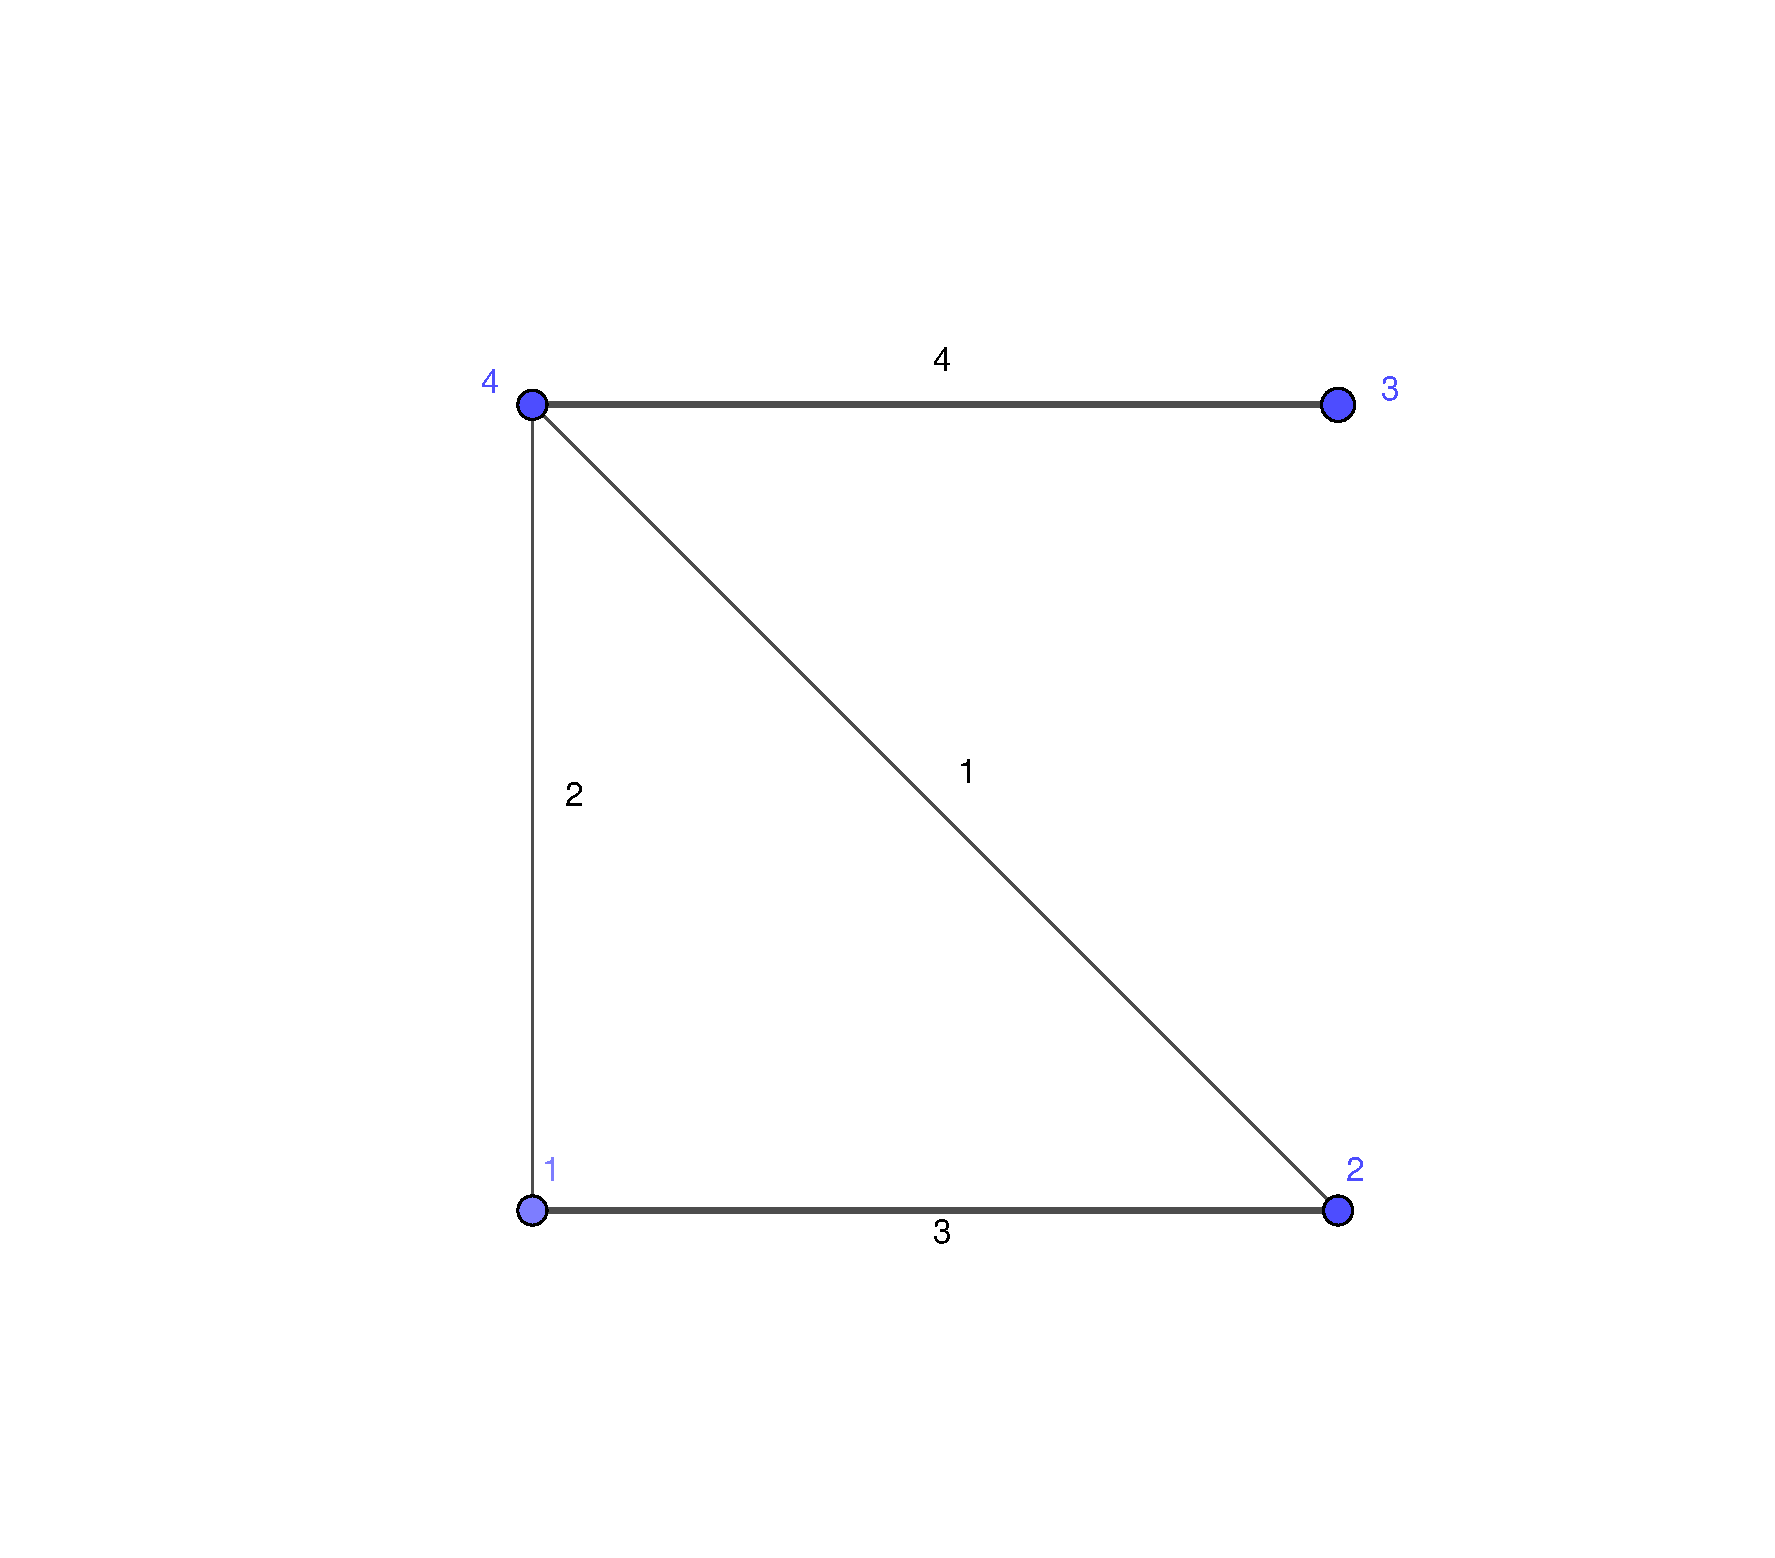
\includegraphics{flussi}

%after having assigned every facility to every location, these algorithms order  $\bm f$ using \texttt{ISORT}, a function of FTN95 which stores on the vector $\bm u_f$ the indices on the same order of the original vector $\bm f$. For example if $\bm f =[5,1,2,4,3]$, then $\bm u_f =[2,3,5,4,1]$. This allows to create the vector $\bm p$, by placing $p(i)=l(u_f)$ for every $i=1,\dots,n$.
%\dafinire

\subsection{\texttt{Greedy1}}


This algorithm represents the first approach we discussed in  section~\ref{sec:EsempioNeos4}. 

Pseudocode~\ref{Pseudocode: Gredy1} describes the algorithm in the symmetric case with $q=0$.




\begin{algorithm}%[htp]
	\KwIn{$n$,$\bm F$, $\bm D$,$n_1$, $n_2$}
	\KwOut{$p$, $z_p$}
	\tcc{initialisation}
	$v_1 \gets n_1$\; 
	$l_1 \gets n_2$\;
	$p_{v_1}\gets l_1$\;
	\tcc{main loop}
	\For{$i=1,\dots,n-1$}{
		Choose $v_{i+1}$, the facility with maximum flow from $f_{i}$\;
		Choose $l_{i+1}$, the location minimizing $\sum_{j=1}^if_{l_{i+1},j}\cdot d_{s,j}$\;
		$p_{v_{i+1}}\gets l_{i+1}$\;
	}
	Evaluate $z_p=z(p)$\;
	\caption[\texttt{Greedy1}]{\texttt{Greedy1} algorithm}
	\label{Pseudocode: Gredy1}
\end{algorithm}


As we said lines 1-3 represent the first assignment.

For the second assignment (and so on), \texttt{Greedy1}   chooses facility  $v_2$ which maximizes the flow from and to the previous ones (line 5); therefore 
\[
v_{i+1} = \argmax \Big\{\max\big\{f_{v_is}\big\},  \max\big\{f_{sv_i}\big\}\Big\}.
\]
 
\noindent After that,  the algorithm chooses location $l_{i+1}$, where facility $v_{i+1}$ will be placed. Location $l_{i+1}$ is chosen such that it minimizes the total flow sent to facilities already in place (line 6). In other words,
\begin{equation}
\begin{split}
l_{i+1} = \argmin\Biggl\{\displaystyle &\sum_{(k,j)\in \Omega} \left(f_{v_i k} d_{sj}+ f_{k v_i}d_{js}\right) \, \Big| \, s \in [n], s \neq l_1  \Biggr\}
\end{split}
\end{equation}


\noindent where $[n]=\{1,2,\dots,n\}$ and $\Omega$ is the set of pairs facility-location already assigned.

This procedure repeats for $i=1,\dots, n-1$ (line 4).

After choosing $v_{i+1}$ and $l_{i+1}$, \texttt{Greedy1} updates the final permutation setting $p_{v_{i+1}}=l_{i+1}$ (line 7).


In the case $q=0$, the algorithm starts again with every possible choice of $n_1$ and $n_2$. The best objective function value is stored.


We implemented \texttt{Greedy1} algorithm in Fortran language and  made it available on \href{https://github.com/Tommaso-Mannelli-Mazzoli/QAP/blob/master/Greedy1.f90}{GitHub}~\cite{Mazzoli2020}.


\subsection{\texttt{Greedy2}}
The second greedy algorithm follows the second approaches in~\ref{sec:EsempioNeos4}. Hence, it is similar to the first one, with the role of facilities and locations exchanged. 

Therefore, using the same notations as before, location $l_{i+1}$ is the closest one to $l_i$.

As regards facilities, $v_{i+1}$ is chosen as


\[
v_{i+1} = \argmin\Biggl\{\displaystyle \sum_{(k,j)\in \Omega} \left( f_{sk}\,d_{l_{i+1}j} +f_{ks}\,   d_{jl_{i+1}} \right)\,
\Big| \, s \in [n], s \neq v_k \, \forall k  \Biggr\}.
\]


\noindent The Fortran code we implemented for \texttt{Greedy2} can be found on \href{https://github.com/Tommaso-Mannelli-Mazzoli/QAP/blob/master/Greedy2.f90}{GitHub}.

\subsection{\texttt{Greedy3}}
The third greedy algorithm follows the third approach described in~\ref{sec:EsempioNeos4}.

For facilities, in each step, the algorithm consider the facility (not already chosen) with highest flow to the previous one.

For locations,  \texttt{Greedy3} considers the closest location (not already chosen) to the current one. 


In pseudo code~\ref{Pseudocode: Greedy3} it is shown the \texttt{Greedy3} algorithm for symmetric case. The Fortran code we implemented and used can be found on \href{https://github.com/Tommaso-Mannelli-Mazzoli/QAP/blob/master/Greedy3.f90}{GitHub}~\cite{Mazzoli2020}.

\begin{algorithm}%[htp]
	\caption{\texttt{Greedy3} algorithm}
	\label{Pseudocode: Greedy3}
	\KwIn{$n$,$\bm F$,$\bm D$,$n_1$, $n_2$}
	\KwOut{$p$, $z_p$}

\tcc{initialisation}
				$f_1 \gets n_1$\; 
				$l_1 \gets n_2$\;
				$p_{f_1}\gets l_1$\;
	\tcc{main loop}
			\For{$i=1,\dots,n-1$}{
	 				$v_{i+1}$ is the facility with maximum flow from $v_i$\;
					$l_{i+1}$ is the closest location to $l_i$\;
				$p_{v_{i+1}}\gets l_{i+1}$\;
			}
		Evaluates $z_p = z(\bm p)$.	
\end{algorithm}

\subsection{Implementation and Comparison}
We compared these three algorithms in order to choose which algorithm use to provide starting permutation for metaheuristic algorithms, that are described in the next chapter.



Table~\ref{tab:ConfrontiGreedy} shows percentage of deviation for various instance of \QAP. The case $q=0$ was chosen for every algorithm.  



\begin{table}
	\footnotesize
	\centering
		\caption[Comparison of Greedy algorithms.]{Comparison of Greedy algorithms. PD is the percentage deviation from the best known solution, $t$ is the running time in seconds.}
	\label{tab:ConfrontiGreedy}
	
	\begin{tabular}{l*{6}{S}}
		\toprule
		Instance& \multicolumn{2}{c}{\texttt{Greedy1}} &  \multicolumn{2}{c}{\texttt{Greedy2}} & \multicolumn{2}{c}{\texttt{Greedy3}} \\
		\cmidrule(lr){2-3}
		\cmidrule(lr){4-5}
		\cmidrule(lr){6-7}
&
{PD} & {$t$} &
{PD} & {$t$} &
{PD} &{ $t$}  \\
\midrule
 \texttt{lipa20a         }  &   3.18  &    0.0 &   5.89  &    0.0 &   3.10  &    0.0\\
\texttt{lipa20b         }  &   0.00  &    0.0 &  29.68  &    0.0 &   0.00  &    0.0\\
\texttt{lipa30a         }  &   2.78  &    0.1 &   4.17  &    0.1 &   2.62  &    0.0\\
\texttt{lipa30b         }  &   0.00  &    0.1 &  29.18  &    0.1 &  12.03  &    0.0\\
\texttt{lipa40a         }  &   2.11  &    0.5 &   3.49  &    0.5 &   2.03  &    0.0\\
\texttt{lipa40b         }  &  15.08  &    0.5 &  30.53  &    0.5 &  19.33  &    0.1\\
\texttt{lipa50a         }  &   1.74  &    1.4 &   3.12  &    1.3 &   1.72  &    0.1\\
\texttt{lipa50b         }  &  16.58  &    1.4 &  30.00  &    1.4 &  22.50  &    0.1\\
\texttt{lipa60a         }  &   1.58  &    3.3 &   2.74  &    3.2 &   1.60  &    0.2\\
\texttt{lipa60b         }  &  21.19  &    3.3 &  32.14  &    3.2 &  23.21  &    0.3\\
\texttt{lipa70a         }  &   1.45  &    6.9 &   2.49  &    6.8 &   1.37  &    0.5\\
\texttt{lipa70b         }  &  21.11  &    6.9 &  32.46  &    7.0 &  25.69  &    0.5\\
\texttt{lipa80a         }  &   1.28  &   13.2 &   2.25  &   12.9 &   1.22  &    0.8\\
\texttt{lipa80b         }  &  22.23  &   13.2 &  33.80  &   13.0 &  26.18  &    0.8\\
\texttt{lipa90a         }  &   1.17  &   23.5 &   1.99  &   22.3 &   1.12  &    1.3\\
   \texttt{lipa90b       }  &  23.31  &   23.1 &  33.51  &   22.6 &  25.23  &    1.2\\
\texttt{sko42           }  &   9.88  &    0.6 &  32.95  &    0.6 &  18.91  &    0.1\\
\texttt{sko49           }  &   8.22  &    1.3 &  31.46  &    1.2 &  16.40  &    0.1\\
   \texttt{sko56           }  &   8.44  &    2.4 &  31.14  &    2.4 &  17.52  &    0.1\\
\texttt{sko64           }  &   7.34  &    4.5 &  28.48  &    4.4 &  15.41  &    0.2\\
  \texttt{sko72           }  &   7.81  &    8.0 &  26.65  &    7.6 &  15.08  &    0.4\\
   \texttt{sko81         }  &   6.51  &   14.2 &  26.39  &   13.5 &  14.44  &    0.6\\
   \texttt{sko90           }  &   7.10  &   23.6 &  24.95  &   23.0 &  13.90  &    0.9\\
\texttt{sko100a         }  &   6.31  &   39.5 &  22.88  &   38.0 &  14.30  &    1.4\\
\texttt{sko100b         }  &   6.60  &   38.8 &  23.82  &   37.0 &  13.52  &    1.2\\
\texttt{sko100c        }  &   6.91  &   38.7 &  24.26  &   36.8 &  13.75  &    1.3\\
\texttt{sko100d        }  &   6.04  &   40.0 &  23.57  &   37.9 &  13.13  &    1.3\\
\texttt{sko100e        }  &   6.69  &   39.8 &  23.98  &   37.1 &  13.42  &    1.2\\
\texttt{sko100f         }  &   6.53  &   40.3 &  23.87  &   38.4 &  14.10  &    1.4\\
		\bottomrule
	\end{tabular}
\end{table}

We can see that all these greedy methods are not very precise, especially on instances \texttt{lipaxxb}. Nevertheless, as we stated at the beginning, they are commonly use only to built an initial guess for more advanced metaheuristic algorithms. 

Moreover, note that \texttt{Greedy3} is much faster than the other two (often with a difference of one order of magnitude), as a confirm of what we supposed. Thus, we will use it for metaheuristic methods presented in the next chapter, despite it shows larger PD values than \texttt{Greedy1}.
\chapter{Metaheuristic algorithms}
\label{chap:Metaheuristic}

\lettrine[lines=3]{\color{BrickRed}T}{he } word heuristic has its origin in the old Greek word $\upepsilon \upnu \uprho \upiota \upsigma \upkappa \upepsilon \acute{\upiota} \upnu  $ (\textit{heuriskein}), which means the art of discovering new strategies (rules) to solve problems. The term \textit{metaheuristic} was introduced by Fred W. Glover in 1986~\cite[p. 541]{Glover1986}, a professor of University of Colorado. In the referred article \textit{Future paths for integer programming and links to artificial intelligence}, he used this term only once in all the document: \begin{quote}\small
	Tabu search may be viewed as a “meta-heuristic” superimposed on another heuristic.
\end{quote}

\begin{wrapfloat}{figure}{O}{0pt}
	\includegraphics[width=.15\textwidth]{Fred_Glover.jpeg}
	\caption[Fred Glover]{\\Fred Glover}
\end{wrapfloat}


\noindent In fact, the Greek suffix \textit{meta} means “upper level methodology''. 


Metaheuristic algorithms were designed in order to solve problems too difficult for the heuristic algorithms. Hence, metaheuristics provide “acceptable” solutions in a reasonable time for solving hard and complex problems in science and engineering.  This explains the significant growth of interest in metaheuristic domain. Unlike exact optimization
algorithms, metaheuristics do not guarantee the optimality of the obtained solutions~\cite{Talbi_2009}.


There are two types of metaheuristic algorithms:
\begin{description}
	\item[Population based] They can be viewed as an iterative improvement in a population of permutations. At first the population is initialized, then a new one is generated and finally these populations are integrated into a new one using a selection procedure. The search process is stopped when a stopping criterion is satisfied. Some of Population based algorithms are Ant Colony Optimization, Genetic Algorithms, Memetic Algorithms~\cite{Talbi_2009}. 
	\item[Single-solution based] While solving optimization problems, single-solution based metaheuristics improve a single solution. They can be viewed as “walks” through neighborhoods or search trajectories through the search space of the problem. Tabu Search, Simulated Annealing, GRASP, Variable Neighborhood Search belong to this class of metaheuristics~\cite{Talbi_2009}.
\end{description}

\noindent There are three central concepts in metaheuristics:
\begin{description}
	\item[Neighborhood] We define a neighborhood of a feasible solution $\pi \in \Sn$ as a generic function $\mathcal N \colon \pi \to \mathcal P(S_n)$ that maps a solution to a set of solutions.
	\item[Intensification] Exploitation of the best solutions. Often this is achieved by doing a local search starting from the current solution.
	\item[Diversification]  Exploration of the search space, in order to escape from local minimum.
\end{description}

We are going to describe three different metaheuristic algorithms:
\begin{itemize}
	\item Tabu Search. We implemented the original algorithm in~\cite{Skorin_Kapov_1990}.
	\item Ant Colony Optimization. We elaborated a new strategy for the diversification phase with respect to~\cite{Gambardella1999}.
	\item Variable Neighborhood Search. We did not find an implementation of this algorithm for QAP in literature; hence, we devised a new implementation \textit{ex novo}. 
\end{itemize}


\section{Tabu search}
\label{sec:Tabu_search}

\subsubsection{Introduction}


The history of Tabu Search (TS)\index{tabu search} is described in the following table.
\begin{center}
\footnotesize
\begin{tabular}{ll}
\toprule
Year & Event \\
\midrule
1986& Tabu Search algorithm is proposed by Glover~\cite{Glover1986}	\\
1990& Skorin-Kapov implements tabu search for QAP~\cite{Skorin_Kapov_1990}\\
1991& Éric Taillard implements \textit{robust tabu search} for QAP~\cite{Taillard_1991}\\
1994&  Battiti and Tecchiolli~\cite{Battiti_1996} implements \textit{reactive tabu search} for \QAP \\
2011 & Misevicius~\cite{Misevicius2011} implements \textit{iterated tabu search} (ITS) for QAP\\
\bottomrule
\end{tabular}
\end{center}

\noindent In his famous paper of 1986, Fred Glover introduced Tabu\footnote{The name comes from Polynesian word \textit{tàpu} that means prohibited.}  Search algorithm as follows:
\begin{quote}\footnotesize
	From an AI point of view, \textit{tabu search }deviates to an extent from what might be expected of
	intelligent human behavior. Humans are often hypothesized to operate according to some sort of
	random (probabilistic) element which promotes a certain level of “inconsistency”. The resulting
	tendency to deviate from a charted course, sometimes regretted as a source of error, can also prove a
	source of gain. Such a mechanism has been postulated to be useful, even fundamental, to human
	ingenuity.
\end{quote}

\noindent TS is one of the most studied and used algorithm for QAP. In several cases, the methods of this class provide solutions very close to optimality and are among the most effective, if not the best, to tackle the difficult problems at hand. Therefore, these successes have made TS extremely popular~\cite{Gendreau2019}.


\begin{wrapfloat}{figure}{O}{0pt}
	\includegraphics[width=.15\textwidth]{Jadranka_Skorin_Kapov}
	\caption[Skorin-Kapov]{\\Jadranka Skorin-Kapov}
\end{wrapfloat}


The main idea of TS is to \textit{forbid} certain moves. This is done in order to escape from local optima. To do this, a \textit{tabu list} was adopted. It is an array of size \textit{s} (called \textit{tabu tenure}), that stores the past evolution of the algorithm.

Since there is a rich variety of strategies and tools, there is a lot of freedom in the implementation of a TS.







The first TS algorithm for QAP was presented by  Jadranka Skorin-Kapov, Stony Brook University, New York. Her algorithm starts with an initial permutation $\pi$ and begin an intensification phase using a local search algorithm; she used the neighborhood ${N}_2$, as defined in section~\ref{def:Intorno}. She forbid the $2$-exchange of two units that were swapped during the previous $s$ iterations, inserting them into the tabu list, i.e., every time a $2$-~exchange is performed, the algorithm inserts the two indices swapped into the tabu list. 


After one year, the \textit{robust tabu search} (roTS) was defined by Éric Taillard, École polytechnique fédérale de Lausanne (Lausanne, Switzerland). Based on Skorin-Kapov work, they used the same neighborhood but a different  tabu list. For every facility $i$ and location $j$, the latest iteration at which the facility $i$ occupied location $j$ is recorded. A $2$-exchange $\pi_{i_1i_2}$ is tabu if  both $i_1$ and $i_2$ are assigned to locations they had occupied in the last $s$ iterations. The tabu tenure varies in a cyclic random manner between a lower value $s_\mathrm{min}=\lfloor 0.9 n \rfloor$ and an high value $s_\mathrm{max}=\lceil 1.1n \rceil$. This value is updated every $2 \cdot s_\mathrm{max}$ iterations.

In 1994, Roberto Battiti and Giampietro  Tecchiolli, Instituto Nazionale di Fisica Nucleare (Trento, Italy),  introduced the reactive tabu search (ReTS). They still used neighborhood $N_2$, but the algorithm evolved in a more complex way. In fact, ReTS \textit{reacts} during the evolution of the search by increasing the tabu tenure when a solution is repeated along the search, and decreasing it if no repetition occurs for a certain number of iterations . They used hashing functions, binary trees, bucket lists as tool to store the solution and to check if a neighbour solution was already visited~\cite{Burkard2012}. The numerical results show that ReTS is competitive with ro-TS in terms of number of iterations performed to reach the best known solution~\cite{Burkard2012}.



In 2011, Alfonsas Misevicius  , Kaunas University of Technology, (Kaunas, Lithuania) implemented~\cite{Misevicius2011} \textit{iterated tabu search} (ITS). He combined the roTS with a special type of mutation. As regards tabu tenure, he differentiated from  Taillard's approach. The tabu tenure $s$ various $s$ in a deterministic way: each time it reached a value $s_\mathrm{max}$, it drops to a lower value $s_\mathrm{min}$. For small size problems ($n\le 50$) he used $s_\mathrm{min}=\lfloor 0.2n \rfloor$ and $s_\mathrm{max}=\lceil 0.4n\rceil$. For larger problems ($n>50$) he used $s_\mathrm{min}=\lfloor 0.1n \rfloor$ and $s_\mathrm{max}=\lceil 0.2n\rceil$.

Now we are going to describe the algorithm in details.

\subsubsection{Description of the algorithm} 

In our implementation, we followed the main idea of Skorin-Kapov's work.

We consider two types of memories:\textit{short-term memory}
 and \textit{long-term memory}.
\begin{description}
	\item[Short-term memory ] This memory consists of a tabu list with tabu tenure $s$. This list is used to prevent revisiting previously visited solutions. This is done in order to achieve diversification.
	
	\item[Long-term memory] This memory stores information on the visited solutions during the search. The idea of long-term memory is to record the frequency with which each movement has been realized since the beginning of the algorithm. In our implementation, long-term memory provide an intensification phase.
\end{description}


An other important ingredient is the \textit{aspiration criterion}. It is essentially a condition that, if holds, allows tabu solutions to be accepted. The most common criterion is  to accepts the tabu moves that generate solutions  better than the best one found so far.


Pseudo code~\ref{Pseudocode: Tabu Search} sketches the idea of the algorithm.

The short-term memory is an array of size $s$ where the best local moves performed are stored. Every time that an improvement of the objective function by a $2$-exchange occurs, the move performed is stored in the tabu list, hence it is prohibited. Since the dimension of  list  is finite, when the list is full the next move will replace the oldest one (this is why it forms the short-term memory: it records only the $s$ previous moves). 
 
  We implemented long-term memory as an $n \times n$ matrix $\bm M =(m_{ij})$. Each entry of $\bm M$ is related to the quality of the $2$-exchange done, e.g., if the $2$-exchange $\{1,2\} \to \{2,1\}$  improves the current solution, then we store this information on $\bm M$, updating the matrix as follows:
  \[M_{12} \gets M_{12}+1 \quad  \text{and} \quad  M_{21}\gets M_{21}+1.\]
  
   



\begin{description}
	\item[Input] Tabu tenure $s$, penalty parameter $\mu$, maximum time $t_\mathrm{max}$.
	\item[Output] The obtained solution $p_\mathrm{best}$ and its objective function value $z_\mathrm{best}$.
\end{description}


\begin{algorithm}
	\footnotesize	
	\KwIn{$n$, $\bm F$, $\bm D$, $\mu$, $s$,  $t_\mathrm{max}$}
	\KwOut{$p_\mathrm{best}$, $z_\mathrm{best}$}	
	\tcc{initialization}
	Build an initial solution $p$ with objective function  $z_p=z(p)$ by \texttt{Greedy3} algorithm\;
	$z_\mathrm{best} \gets z_p$\;
	$ p_\mathrm{best} \gets \bm p$\;
	$\bm M \gets \bm 0$\;
	$\tilde{\bm D} \gets \bm D$\;
	\tcc{main loop}
	Call \texttt{CPU\_TIME}  $t$\;
	\While{$t < t_\mathrm{max} $}
	{\label{alglinea:dmin}
		\tcc{improvement of the current solution}
			$d_\text{min} \gets 0$\;
			Starting from $p$, search an admissible local $2$-optimum $p_\mathrm{temp}\in {N}_2(p)$ with objective function value $z_\mathrm{temp}$. This is obtained by a $2$-exchange of indices $(j_1,j_2)$\;
			$d_\mathrm{min} \gets \Delta(p;j_1,j_2)$\;
			\tcc{update short-term memory}
			Add the pair $(j_1,j_2)$ to tabu list\;
			
			
			\If{$d_\mathrm{min} < 0$ }{
				$z_p \gets z_\mathrm{temp}$\;
				$p \gets p_\mathrm{temp}$\;
				\tcc{update long-term memory}
				$m_{j_1j_2}  = m_{j_1j_2}  +1$\;
				$m_{j_2j_1}  = m_{j_2j_1}  +1$\;
				\If{$z_p<z_\mathrm{best}$}{
					$z_\mathrm{best} \gets z_p$\;
					$p_\mathrm{best} \gets p$\;
				}
				Call \texttt{CPU\_TIME}  $t$\;
				Go to~\ref{alglinea:dmin}\;
			}
			\tcc{create a new solution using long-term memory}
			$\tilde{\bm D} \gets  \tilde{\bm D} + \mu \bm M $ \;
			Use \texttt{Greedy3} with matrices $\bm F$ and $\tilde{\bm D}$ to create a new permutation $p$ with objective function $z_p$\;
			Call \texttt{CPU\_TIME} $t$\;
		}
		\caption{Tabu search}
		\label{Pseudocode: Tabu Search}
	\end{algorithm}


\subsubsection{Initialization}%\mbox{}\\


At first algorithm builds an initial permutation. In our implementation it is provided by the by \texttt{Greedy3} method (line 1). The output permutation and its objective function provided by \texttt{Greedy3}  are denoted by $p$ and $z_p$.
 
 The long-term matrix is initialized as the null matrix (line 4).
 A copy of distance matrix $\bm D$ is stored in matrix $\tilde{\bm D}$ (line 5).

\subsubsection{Improvement of the current solution}


The algorithm looks for an improvement of the current solution (lines 9-10). This is done in our implementation by a modified version of \texttt{2optBest} algorithm. 



The difference with \texttt{2optBest} algorithm is that not every move is allowed. At each step, TS controls if the current indices $i_1$ and $i_2$ belong to tabu-list. If this is the case, \texttt{2optBest} variant skips to the next pair of indices.

It is possible to overcome the tabu restriction for a pair $(j_1,j_2)$ if the $2$-exchange $\{j_1,j_2\}\to \{j_2,j_1\}$ improves the best solution  obtained by far $p_\mathrm{best}$.  

The term $d_\mathrm{min}$ is stored (line 10). It is the best improvement of the objective function value obtained.

If $d_\mathrm{min}=0$, this means that the best $2$-exchange found does not improve the current solution. Therefore, $p_\mathrm{temp}$ is an admissible local optimum. The term \textit{admissible} means that it does not belong to the tabu list, or it belongs but provides an improvement of the best permutation found so far $p_\mathrm{best}$.

On the other hand, if $d_\mathrm{min}<0$, then there is indeed an improvement of the objective function value.
Suppose that $\{j_1,j_2\}\to \{j_2,j_1\}$ is the best  admissible $2$-exchange. Then, the $2$-exchange is applied and its objective function value is updated (lines 13-14).

Moreover, if the permutation after the $2$-exchange is the best found so far, the algorithms update $p_\mathrm{best}$ and $z_\mathrm{best}$ (lines 18-20).


This procedure repeats until the actual permutation $p$ cannot be improved any more ($d_\mathrm{min}\ge 0$).


\subsubsection{Updating of the memories}

The short-term memory is updated: the two indices $j_1$ and $j_2$ enter in the tabu list (line 11).

If the tabu list is full, it starts again by substituting the first two index of the list with $j_1$ and $j_2$.
This idea was taken from Skorin-Kapov~\cite{Skorin_Kapov_1990}.

As regards long-term memory, the matrix $\bm M$  is updated by increasing  $m_{j_1,j_2}$ and $m_{j_2,j_1}$ by $1$ (lines 15-16). This memory, unlike tabu list, is never reset its value. Therefore, the indices $j_1$ and $j_2$ remain in $\bm M$ until the end of the algorithm. 

\subsubsection{Creation of a new permutation}

 At this point  the matrix $\tilde{\bm D}$ is updated as $\tilde{\bm D} \gets \tilde{\bm D}+ \mu \bm M$ where $\mu$ is an input penalty parameter (line 24).
 
In our runs, we set 
   
   \begin{equation}
   	\label{eq:ParametroMu}\mu = k \cdot \frac{1}{n^2} \sum_{j=1}^n\sum_{i=1}^n d_{ij}.
   	\end{equation}
   
   \noindent This allow us to adapt the magnitude of $\mu \bm M$  to the one of matrix $\bm D$; 
 
  If $\mu > 0$, the algorithms increases distance between locations frequently swapped, therefore tries to achieve diversification. 
 
 On the other hand, if $\mu < 0$, then distance between locations frequently swapped decreases, hence the algorithm stimulates frequent moves to be chosen.
 


Finally, a constructive algorithm is used to create another solution $p^*$ from the updated matrix $\bm D$. Here the algorithm starts again, setting $p\gets p^*$. 

Note that the only \texttt{Greedy3} algorithm uses the updated matrix $\tilde{\bm D}$, the rest of the algorithm still uses the original distance matrix $\bm D$.



\subsection*{Implementation and parameters calibration}
We implemented algorithm~\ref{Pseudocode: Tabu Search} in Fortran language. The code can be found on \href{https://github.com/TDS-Firenze/QAP/blob/master/TABU_SEARCH.f90}{GitHub}~\cite{Mazzoli2020}.

Since the dimension of the instances are very different, we are going to do two separate calibrations: one for small dimensions ($n < 50$) and an other one for large dimensions ($n \ge 50$).

The algorithm stops whenever the execution time exceeds the input value $t_\mathrm{max}$. We chose $t_\mathrm{max}=\SI{30}{\second}$ for $n<50$ and $t_\mathrm{max}=\SI{60}{\second}$ for $n\ge 50$.

Finally, we run the code on a   i$7$-$9750$H processor with \SI{2.60}{\giga\Hz} clock frequency.

The parameters we have to calibrate are 
\begin{itemize}
	\item the parameter $k$ used in~\eqref{eq:ParametroMu}; 
	\item the size of tabu list $s$; if its value is too small, cycling may occur in the
	search process while if its value is too large, appealing moves may be forbidden and leading to	the exploration of lower quality solutions, producing a larger number of iterations to find the solution desired.
\end{itemize}


To calibrate them, we vary the parameters in a  reasonable range and then we took the values providing best objective function values at average. Like the previous chapter,  we evaluated the Percent Deviation (PD) from the optimal solution.

After some tests we found that the bests values of $k$ were between $-1$ and $-2$, hence we explored it more deeply. Finally, the range of tested parameter values  is 
\begin{itemize}
	\item $k \in \{1, -1,-1.2, -1.4, -1.6, -1.8, -2, -5, -10, -20 \}$
	\item $s \in \{8,10,15,20,25,50,100,200\} $
\end{itemize}



The following pages contain tables where we highlighted in \colorbox{green!40}{green} the optimal solution (or the best known solution) and  in \colorbox{blue!30}{blue} good solutions, even if they were not the optimal.


\subsubsection{Small dimension}
Instances used to calibrate are 
\begin{description}
	\item[\texttt{Tai12a}] We achieved the optimum for several $(k,s)$ (table~\ref{TS:Tai12a})
	. In  most of the cases, the percent error of the solution is less than $4\%$.
	\item[\texttt{Chr20c}] We achieved the optimum for $s = 20,50$ and $k = -1.8$ (table~\ref{TS:chr20c})
	. Other good result were obtained  for  $s = 150$ and $k = -1.8, -2, -5, -10, -20$.
	\item[\texttt{Nug30}] The best solution we achieve (Table~\ref{TS:Nug30}) 
	has a percent error of  $0.03\%$  with $k = -5, -10, -20$ and $s = 20$. All other solutions are pretty good, since they always are under $2\%$ of percent error, except for $k = 1$.
\end{description}




\subsubsection{Large dimension}
We used the following instances:



\begin{description}
	\item[\texttt{Lipa60b}] As we can see in table~\ref{TS:Lipa60b} 
we reached the optimal solution $7$ times: for $\mu = -1$ and $s= 25$, $ 50$, $100$, $150$, for  $\mu = -1.2$ and $s = 8$ and finally for $s = 150$ and $\mu = -1.8$. The instance is asymmetric.
	\item[\texttt{Wil100}]The optimal solution is not known. Every solutions we found has less than $1\%$ of error from the best known solution (which is $64$).
	\item[\texttt{Esc128}] As we can see in table~\ref{TS:Esc128}, 
	We reached the optimum many times. Notice that TS provides optimal solution for every $s$ if $k=-1.8$,$-2$,$-5$,$-10$.

\end{description}

\subsubsection{Conclusions}
%As we can see 
The choice of $k=1$ did not perform well in any instance. This reflects the fact that, for our TS algorithm, intensification is a better strategy than diversification.

For small dimension, we decided to choose $s=20$ and $k=-1.8$, since it provides the optimal solution for \texttt{Chr20c} and for \texttt{Tai12a} and \texttt{Nug30} the sum of the error is minimal: only $2.9\%$.


For large dimension, we chose $s=20$ and $k = -1.4$, since it provides the optimal solution for \texttt{Lipa60b} and \texttt{Esc128}, while only an error of $0.48\%$ for \texttt{Wil100}.


\begin{table}%[p]
	\scriptsize
	\centering
	\begin{tabular}{l*{10}{S[table-format =2.2]}}
		\toprule
		$s$ & \multicolumn{10}c{{$k$}} \\
		\cmidrule{2-11} 
		&    1  &    -1  &  -1.2  &    -1.4    &    -1.6  & -1.8  &    -2  &-5  &
		 -10  &-20    \\
		\midrule
		$8 $  & 6.38 & \best 0 &\best 0 & \best 0 & \best 0 & \best 0 & \best 0 & 3.84  &  3.84 & 3.84\\
		$10$  & 6.30 & \colorbox{green!40}{$0$} & \colorbox{green!40}{$0$} & \colorbox{green!40}{$0$} & \best 0 & \best 0 & \best 0 &  2.08 & \colorbox{green!40}{$0$}& \colorbox{green!40}{$0$}\\
		$15 $ & 6.30 &\colorbox{green!40}{$0$} & \best 0 & \best 0 & \best 0 & \best 0  & \colorbox{green!40}{$0$} & \colorbox{green!40}{$0$} & \colorbox{green!40}{$0$}& \colorbox{green!40}{$0$}\\
		$20$  & 6.30  & \best 0 & \best 0 & \best 0 & 2.80 & 2.80  &2.08   & 2.08 &2.08  &2.08 \\	
		$25$  & 6.30  & 2.80 & 2.80 & 2.08 & \best 0 & 2.08 &  \best 0  & \best 0  & \best 0  &\best 0  \\
		$50$ & 6.30  & 3.84 & 3.84 & 2.80 & 2.80 & 2.08 & 3.84 & \best 0   & \best 0  &\best 0 \\
		$100$ & 6.30  & \best 0  & 2.08 & 2.08 & 2.08 & 2.08 & \best 0   & 2.08 &2.08  &2.08 \\
		$150$ & 6.30  & 6.89 & 6.89 & 2.08 & 2.08 & 2.08 & \best 0  & \best 0 &2.80  &2.80 \\
		\bottomrule
	\end{tabular}
	\caption{Tabu Search for  \texttt{Tai12a}}
	\label{TS:Tai12a}
\end{table}

\begin{table}
	\scriptsize
	\centering
	\begin{tabular}{l*{10}{S[table-format =2.2]}}
	\toprule
	$s$ & \multicolumn{10}c{{$k$}} \\
	\cmidrule{2-11} 
		&    1  &    -1  &  -1.2  &    -1.4    &    -1.6  & -1.8  &    -2  &-5  & -10  &-20    \\
	\midrule
		$8$   & 41.61 & 6.82  & 20.11 & 6.04 & 18.92 & 13.75 &13.75 & 13.75 & 13.75 & 13.75  \\
		$10$  & 41.61 & 21.67 & \colorbox{blue!30}{$4.72$} & 18.22 & 15.90 & 19.37 & 19.37 & 19.37 & 19.37 & 19.37  \\
		$15$  & 39.57 & 20.72 & 18.58 & 11.51 & 24.62 & 18.98 & 18.98 & 18.98 & 18.98 & 18.98  \\
		$20$  & 39.57 & 18.88 & 20.18 & 19.30 & \colorbox{blue!30}{$4.72$} & \best 0 &  19.37 & 19.37 & 19.37 & 19.37  \\
		$25$  & 39.57 & 18.53 & 19.81 & 22.43 & 19.37 & 20.80 & 20.80 & 20.80 & 20.80 & 20.80  \\
		$50$  & 39.57 & 13.75 & 15.90 & 15.20 & 16.69 & \best 0 & 28.72 & 28.72 & 28.72 & 28.72  \\
		$100$ & 36.22 & 17.83 & 18.82 & 18.22 & 18.53 & 20.80 & 20.61 & 20.61 & 20.61 & 20.61  \\
		$150$ & 36.22  & 26.79 & 18.89 & 18.22 & 16.39 & \colorbox{blue!30}{$4.74$}  & \colorbox{blue!30}{$4.74$} & \colorbox{blue!30}{$4.72$}  & \colorbox{blue!30}{$4.72$}  & \colorbox{blue!30}{$4.72$} \\
		\bottomrule
	\end{tabular}
	\caption{Tabu Search for  \texttt{Chr20c}}
	\label{TS:chr20c}
\end{table}

\begin{table}
	\footnotesize
	\centering
	\begin{tabular}{l*{10}{S[table-format =2.2]}}
		\toprule
		$s$ & \multicolumn{10}c{$k$} \\
		\cmidrule{2-11} 
		&    1  &    -1  &  -1.2  &    -1.4    &    -1.6  & -1.8  &    -2  & -5  &
		-10  &-20    \\
		\midrule
		$8$   & 2.45 & 0.98 & 1.27 & 0.78 & 1.44 & 0.95 & 0.95 & 1.96 & 1.96 & 1.96  \\
		$10$  & 2.45 & 1.08 & 0.36 & 0.78 & 1.40 & 1.67 &  1.67 & 1.24 & 1.24 & 1.24  \\
		$15$   & 2.45 & 0.69 & 1.08 & 0.98 & 0.49 & 0.88 & 0.88 & 1.34 & 1.34 & 1.34  \\
		$20$  & 2.45 & 0.85 & 0.88 & 1.47 & 1.47 & 0.82 & 1.86 & \colorbox{blue!30}{$0.10$}  & \colorbox{blue!30}{$0.10$} & \colorbox{blue!30}{$0.10$}  \\
		$25$  & 2.45 & 0.95 & 0.98 & 0.59 & 1.24 & 0.69 & 0.91 & 0.88 & 0.88 & 0.88  \\
		$50$  & 2.45 & 1.05 & 0.62 & 1.14 & 0.46 & 0.75 & 0.69 & 1.01 & 1.01 & 1.01  \\
		$100$ & 2.02 & 0.85 & 0.98 & 0.52 & 1.27 & 1.11 & 1.18 & 0.52 & 0.52 & 0.52  \\
		$150$ & 2.45 & 1.08 & 1.27 & 1.24 & 0.69 & 1.21 & 1.08 & 0.95 & 0.95 & 0.95  \\
		\bottomrule
	\end{tabular}
	\caption{Tabu Search for \texttt{Nug30}}
	\label{TS:Nug30}
\end{table}


\begin{table}
\scriptsize
	\centering
	\begin{tabular}{l*{10}{S[table-format =2.2]}}
		\toprule
		$s$ & \multicolumn{10}c{$k$} \\
		\cmidrule{2-11} 
		&    1  &    -1  &  -1.2  &    -1.4    &    -1.6  & -1.8  &    -2  & -5  &-10  &-20    \\
		\midrule
		$8$  &  19.90 & 19.13    & \best 0 & 19.03   & 19.15 & 19.05   & 19.05 & 19.05 & 19.05 & 19.05    \\
		$10$ &  19.90 & 19.19    & 18.92   & 18.82   & 18.91 & 19.02   & 19.02 & 19.02 & 19.02 & 19.02    \\
		$15$ &  19.54 & 19.09    & 18.90   & 19.44   & 18.92 & 19.11   & 18.92 & 18.92 & 18.92 & 18.92    \\
		$20$ &  19.90 & 19.09    & 19.03   & \best 0 & 18.89 & 19.14   & 19.21 & 18.89 & 18.89 & 18.89    \\
		$25$ &  19.90 & \best 0  & 18.90   & 19.44   & 18.92 & 19.11   & 18.92 & 18.92 & 18.92 & 18.92    \\
		$50$ &  19.90 & \best 0  & 19.14   & 18.86   & 18.90 & 19.03   & 19.03 & 19.03 & 19.03 & 19.03   \\
		$100$&  19.83 & \best 0  & 19.00   & 19.06   & 19.03 & 19.08   & 19.03 & 19.08 & 19.08 & 19.08   \\
		$150$&  19.58 & \best 0  & 18.87   & 19.10   & 19.04 & \best 0   & 19.042 & 19.04 & 19.04 & 19.04   \\
		\bottomrule
	\end{tabular}
	\caption{Tabu Search for  \texttt{Lipa60b}}
	\label{TS:Lipa60b}
\end{table}

\begin{table}
\scriptsize
	\centering
	\begin{tabular}{l*{10}{S[table-format =2.2]}}
		\toprule
		$s$ & \multicolumn{10}c{$k$} \\
		\cmidrule{2-11} 
		&    1  &    -1  &  -1.2  &    -1.4    &    -1.6  & -1.8  &    -2  & -5  &-10  &-20    \\
		\midrule
		$8$   & 0.69 & 0.60 & 0.69 & 0.54 & 0.65 & 0.75 & 0.75 & 0.47 & 0.47 & 0.47 \\
		$10$  & 0.68 & 0.60 & 0.69 & 0.64 & 0.65 & 0.77 & 0.63 & 0.47 & 0.47 & 0.47 \\
		$15$  & 0.73 & 0.60 & 0.72 & 0.60 & 0.65 & 0.82 & 0.65 & 0.59 & 0.59 & 0.59 \\
		$20$  & 0.83 & 0.60 & 0.72 & 0.48 & 0.65 & 0.67 & 0.71 & 0.79 & 0.79 & 0.79 \\
		$30$  & 0.87 & 0.60 & 0.74 & 0.62 & 0.58 & 0.69 & 0.66 & 0.72 & 0.72 & 0.72 \\
		$50$  & 0.67 & 0.60 & 0.74 & 0.62 & 0.58 & 0.69 & 0.66 & 0.72 & 0.72 & 0.72 \\
		$100$ & 0.59 & 0.60 & 0.62 & 0.54 & 0.65 & 0.60 & 0.68 & 0.55 & 0.55 & 0.55 \\
		$150$ & 0.66 & 0.60 & 0.70 & 0.65 & 0.58 & 0.64 & 0.69 & 0.69 & 0.69 & 0.69 \\
		\bottomrule
	\end{tabular}
	\caption{Tabu Search for \texttt{Wil100}}
	\label{TS:Wil100}
\end{table}

\begin{table}
\scriptsize	
\centering
	\begin{tabular}{l*{10}{S[table-format =2.2]}}
		\toprule
		$s$ & \multicolumn{10}c{$k$} \\
		\cmidrule{2-11} 
		&    1  &    -1  &  -1.2  &    -1.4    &    -1.6  & -1.8  &    -2  & -5  &-10  &-20    \\
		\midrule
		$8$ &9.38 & 3.31 & 3.13 & 3.13 & \best 0 &  \best 0 & \best 0 & \best 0 & \best 0 & \best 0  \\
		$10$& 9.38 & 3.13 & \best 0 & \best 0 & \best 0 & \best 0 & \best 0 & \best 0 & \best 0 & \best 0 \\
		$15$& 9.38 & 3.13 & \best 0 & \best 0 & \best 0 & \best 0 & \best 0 & \best 0 & \best 0 & \best 0\\
		$20$& 9.38 & 3.13 & \best 0 & \best 0 & \best 0 & \best 0 & \best 0 & \best 0 & \best 0 & \best 0 \\
		$25$&  9.38 & 3.13 & \best 0 & \best 0 & \best 0 & \best 0 & \best 0 & \best 0 & \best 0 & \best 0 \\
		$50$ & 9.38 & 3.13 & \best 0 & \best 0 & \best 0 & \best 0 & \best 0 & \best 0 & \best 0 & \best 0 \\
		$100$& 9.38 & 3.13 & \best 0 & \best 0 & \best 0 & \best 0 & \best 0 & \best 0 & \best 0 & \best 0 \\
		$150$& 9.38 & 3.13 & 3.13 & 3.13& 9.38 & \best 0 & \best 0 & \best 0 & \best 0 & \best 0\\
		\bottomrule
	\end{tabular}
	\caption{Tabu Search for \texttt{Esc128}}
	\label{TS:Esc128}
\end{table}




\newpage
\afterpage{\clearpage}
\section{Ant Colony Optimization}
\label{sec:Ant_Colony_Optimization}

Ant Colony Optimization algorithm (ACO) was initiated by Dorigo  in 1991. The principle of this method is based on the way Argentine ants \textit{Iridomyrmex humilis} search for food and find their way back to the nest~\cite{Goss1989}. At first, ants explore the area surrounding their nest at random. Then, during the return trip, ants leave a pheromone trail on the ground, in order to guide other ants toward the source of food. The quantity of pheromone left depends on the amount of food found. Pheromone trail evaporates if no one pass there any more.


This algorithm is population based. Hence, at first $m$ initial solutions (the ants) are generated. Then, it comes intensification: each ant is improved in a local search phase. Finally, before the start of the next iteration, the pheromone trail is updated reflecting the \virgolette{experience} of the ants.

\subsection{Hybrid Ant System}


Inspired by Gambardella, Taillard and Dorigo~\cite{Gambardella1999} we implemented a variant of ACO known as Hybrid Ant System (HAS). Nevertheless, we will still refer to this algorithm as ACO.

In this implementation the pheromone trail is a $n \times n$ matrix $\bm T=(\tau_{ij})$, where the entry $\tau_{ij}$ measures how good is assigning facility $i$ to location $j$.
Pseudo code~\ref{Pseudocode : ACO} outlines main steps of ACO.
\begin{algorithm}
	\KwIn{$n$, $\bm F$, $\bm D$, $t_\mathrm{max}$}
	\KwOut{$p_\mathrm{best}$, $z_\mathrm{best}$}
	\caption{ACO algorithm}
	\label{Pseudocode : ACO}
Initialize pheromone trail matrix $\bm T$\;

\While{$t < t_\mathrm{max}$}{
Generate $m$ random initial permutation $\pi^1,\dots,\pi^m$\;
Improve $\pi^1,\dots,\pi^m$ with \texttt{2optFirst} algorithm\;
Let $\pi_\mathrm{best}$ be the best permutation among $\pi^1,\dots,\pi^m$\;
\tcc{solution manipulation}
\For{$k=1,\dots,m$} 
    {Apply $R$  $2$-exchanges to $\pi^k$ to obtain $\hat\pi^k$\;
     Apply \texttt{2optFirst} to $\hat\pi^k$ to obtain $\tilde{\pi}^k$\;
\tcc{intensification}
\eIf{intensification is active}
{$\pi^k\gets $ best permutation between $\pi^k$ and $\tilde{\pi}^k$\;}
{$\pi^k \gets \tilde{\pi}^k$}
}
Deactivate intensification\;
\If{exists $k$ such that $z(\pi^k)< z_\mathrm{best}$}{
Update $\pi_\mathrm{best}$\;
Activate intensification\;}
\tcc{pheromone trail updating}
Update pheromone trail matrix $\bm T$\;
\tcc{diversification}
\If{$S$ loops have been performed without improving $\pi_\mathrm{best}$}{Perform a diversification: $\bm T \gets \bm 0$\;}
}
\end{algorithm}

\subsection{Implementation}

\subsubsection{Pheromone trail initialization}


In the original algorithm by Gambardella et al~\cite{Gambardella1999}, pheromone trail matrix $\bm T$ was initialized by setting every component to the same value $\tau_0=\frac{1}{100 z_\mathrm{best}}$, where $z_\mathrm{best}$ is the best know value of the objective function. 

Instead, we tried another approach: two matrices $\bm M_1$ and $\bm M_2$ are used and then combined to form matrix $\bm T$. 

First, the two matrices $\bm M_1$ and $\bm M_2$ are initialized to $0$. 

Then, $n$ initial permutations are built, by setting
\[
\pi_i= [i,i+1,\dots,n,1,2,\dots,i-1] \qquad \forall i\in{1,\dots,n}
\]
After that, for every permutation $\pi_i$,  \texttt{2optBest} algorithm is applied with the following remarks:
\begin{itemize}
	\item Every $2$-exchange made (hence, every improvement of the solution) is stored: if indices $p$ and $q$  of $\pi_i$ are swapped, therefore  we update the matrix $\bm M_2$ as follows:
	\begin{align*}
	M_2(p,\pi_i(p)) &\gets 	M_2(p,\pi_i(p)) -1, &\quad  M_2(q,\pi_i(q)) &\gets 	M_2(q,\pi_i(q)) -1,\\
	M_2(p,\pi_i(q)) &\gets 	M_2(p,\pi_i(q)) +1, &\quad  M_2(q,\pi_i(p)) &\gets 	M_2(q,\pi_i(p)) +1.
	\end{align*} 
	Finally, since we want $\bm M_2$ to be positive, we set $\bm M_2 \gets \bm M_2 + \min(\bm M_2)$.
	\item At the end of  local search procedure, a final permutation $\tilde{\pi}_i$ is found. Thus, $\bm M_1$ is updated as follows:
	\[
	M_1(r,\tilde{\pi}_i(r)) \gets 	M_1(r,\tilde{\pi}_i(r))+1 \quad \forall r \in \{1,\dots,n\}.
	\]
\end{itemize}

\noindent Finally, pheromone trail matrix $\bm T$ is built summing $\bm M_1$ and $\bm M_2$: \[ \bm T \gets \bm M_1 + \bm M_2.\]
In a nutshell, $\tau_{ij}$ tells us how good is the assignment $\pi(i)=j$. 
\subsubsection{Initialization of solutions}


As in~\cite{Gambardella1999}, $m$ random permutations are chosen. Each permutation is optimized using a local search procedure. Gambardella~\cite{Gambardella1999} used a variant of first improvement algorithm. Instead, we used our \texttt{2optFirst} algorithm.

\subsubsection{Manipulation of solutions}


In~\cite{Gambardella1999}, a number of $R$ $2$-exchanges are applied to each permutation $\pi^k$. These operations provides $m$ new permutations $\hat{\pi}^1,\dots, \hat \pi ^m$. We followed the same procedure. These $R$ swaps are performed as follows:


First, an index $r$ is chosen, randomly between $1$ and $n$.

Then, a second index $s \neq r$ is chosen and the elements $\pi^k_r$ and $\pi^k_s$ are swapped in the current solution $\pi^k$.

The second index $s$ is chosen according to following policy:
\begin{itemize}
	\item With probability given by a parameter $q$, $s$ is chosen such that $\tau_{r\pi_s}+\tau_{s \pi_r}$ is maximum. This means that $s$ is the best $2$-exchange for $r$ we can do, according to pheromone trail matrix $\bm T$.
	\item With probability $(1-q)$, $s$ is chosen with a probability proportional to the values contained in $\bm T$. More precisely, $s$ is chosen with probability
	\begin{equation}
	\label{eq:ACOdensity}
	\frac{\tau_{r\pi_s}+\tau_{s \pi_r}}{\sum_{j \neq r}\left(\tau_{r\pi_j}+\tau_{j \pi_r}\right)}.
	\end{equation}
\end{itemize}
Note that setting $M_2\ge 0$ allows $\tau_{ij}$ to be positive. Therefore,  expression~\eqref{eq:ACOdensity} is indeed a density of probability.  

After the $2$-exchange, \texttt{2optfirst} algorithm is applied to every permutation $\hat{\pi}^k$, obtaining $m$ $2$-optima: $\tilde{\pi}^1\dots, \tilde{\pi}^m$.

\subsubsection{Intensification}

The intensification mechanism is activated when the best solution produced so far $\pi_\mathrm{best}$  has been improved. Intensification remains active while at least one solutions is improved during an iteration. Therefore:
\begin{itemize}
	\item If intensification is active, then each permutation starts its next iteration as the best permutation between $\pi^k$ and $\tilde{\pi}^k$.
	\item If intensification is not active, then the permutation is maintained as~$\tilde{\pi}^k$.
\end{itemize}

\subsubsection{Pheromone trail update}
Pheromone trail is updated by taking into account only the best solution~$\pi_\mathrm{best}$. 

Firstly, the pheromone trail $\bm T$ is weakened by setting $\tau_{ij}= (1-\alpha)\cdot \tau_{ij}$ where $0<\alpha<1$ is a parameter that controls \textit{evaporation} of the trail. A value of $\alpha$ close to $0$ implies that pheromone is more persistent, while a value close to $1$ implies high degree of evaporation (thus, a shorter memory of the system).

Secondly, $\bm T$ is reinforced by considering the best permutation obtained so far $\pi_\mathrm{best}$. 
In~\cite{Gambardella1999}, authors update the pheromone trail $\bm T$ as follows: 
\begin{equation}
\tau_{i\pi_\mathrm{best}(i)} \gets \tau_{i \pi_\mathrm{best}(i)} + \frac{\beta}{z_\mathrm{best}} \qquad \forall i \in \{1,\dots,n\}.
\end{equation}
Instead, we followed an other approach: The algorithm builds matrices $\bm M_1$ and $\bm M_2$ in the same way of pheromone trail initialization, but only considering $\pi_\mathrm{best}$ instead of all the $m$ permutations.

 Finally, we update $\bm T$ as follows:
 
  \begin{equation}\bm T  \gets\bm T  + \left(\bm M_1 + \bm M_2 \right).
\end{equation}

\subsubsection{Diversification}
Diversification mechanism is activated if, during the last $S$ loops, no improvement to the best generated solution is detected.
Diversification consists in erasing all the information contained in the pheromone trail and in randomly generating other $m$ solutions (line 22).

\subsubsection{Complexity}
The complexity of the algorithm can be evaluated as follows: most time consuming part of the algorithm is the local search procedure, which has a computational cost of $O(n^3)$ operations. This is repeated $Im$ times, where $I$ is the number of loops performed. Hence, the total cost of ACO is $O\left(Imn^3\right)$.

\subsection{Parameters calibration}
Table~\ref{tab:ACOParam} shows us the parameters that must be calibrated, the tested ranges and the chosen values.

\begin{table}[htp]
	\small
	\centering
	\caption{Parameters of ACO algorithm}
	\label{tab:ACOParam}
	\begin{tabular}{lccl}
		\toprule
		Name & Symbol & Value & Range tested \\
		\midrule
		Probability & $q$ & $0.85$ &$\{0.15, 0.50, 0.85\}$ \\
		Number of $2$-exchanges performed & $R$& $2$ &$\{5,10,15\}$\\
		Evaporation & $\alpha$ & $0.25$ & $\{0.15, 0.25\}$\\
		Maximum number of non improving loops & $S$&  $5n$ & $\{n, 2n, 5n\}$\\
		Number of ants & $m$ & $10$  & $\{5,10,20\} $\\
		
		
		\bottomrule
	\end{tabular}
\end{table}


We tested various values of each parameters for $6$ instances: \texttt{tai12a}, \texttt{chr20c}, \texttt{nug30}, \texttt{lipa60b}, \texttt{wil100} and \texttt{esc128}.

In this case, we did not make any distinctions between small and large dimensions instances, since no substantially differences were found.




We chose a number of ants $m$ equal to $10$, to limit the computation time required for the algorithm. 

The parameter $S$ was set equal to $5n$. For $S \le n$, the algorithm provides poorly solution with high percentage deviation, even for small dimension instances.

As regards the other parameters, they were experimentally found  to be good and robust for the instance tested, providing an output permutation with less than $1\%$ of PD. 



\newpage

\section{Variable neighborhood Search}
\label{sec:Variable_neighborhood_Search}

\subsubsection{Introduction}


\noindent The Variable Neighborhood Search algorithm (VNS) was introduced by Pierre Hansen and Nenad Mladenovic in 1997~\cite{Mladenovic1997} for the Traveling Salesman Problem (TSP). The literature of VNS for QAP is not as extended as for Tabu Search or Ant Colony Optimization. 

The main idea of the algorithm is to use several neighborhood structures and, when a local optimum is found, to move from one to another.

Now, we present some essential definitions and facts about neighborhood structures. More detail can be found in~\cite[Ch. 3]{Gendreau2019}.

Let us start with two definitions.

\begin{defi}[Neighborhood structure]
	A function $\mathcal N \colon \Sn \to \mathcal P(\Sn)$ that maps  a feasible solution $\pi \in \Sn$ to a set of a solutions $\mathcal N(\pi) \subseteq \Sn$ is called a \textit{neighborhood  structure}.
\end{defi}

\begin{defi}[Local optimum]
	A solution $\pi^*$ is called a \textit{local optimum} with respect to the neighborhood structure $\mathcal N$ if there is no feasible solution $\sigma \in \mathcal N(\pi^*)$ such that $z(\sigma) \le z(\pi^*)$.
\end{defi}
Essentially, we can consider  $\mathcal N(\pi)$ as a set of permutations \textit{close} to $\pi$.

Therefore, the operator $\mathcal N$ allows us to obtain new feasible solutions realizing a determined operation on an initial solution.

Note that neighborhoods $N_r$ defined by~\eqref{def:Intorno} are an example of neighborhood structures, since they map a permutation $\pi$ into the set of permutations that can be reached by $\pi$ by a $r$-exchange.

\subsection{Local search}

\subsubsection{Description of the algorithm}

This procedure is a generalization of the local search algorithms discussed in section~\ref{sec:LocalSearch}. 

Pseudo code~\ref{Pseudocode:LocalSearch} shows the local search algorithm. 


\begin{algorithm}\footnotesize
	\KwIn{An initial permutation $s_1$, a neighborhood structure $\mathcal N$}
	\KwOut{A local optimum $s^*$ w.r.t. $\mathcal N$}
	\Repeat{a local optimum  $s^*$ is found}{
		Examine $\mathcal N(s_1)$\;
		\eIf(){exists $s_2\in \mathcal N(s_1)$ such that $z(s_2)\le z(s_1)$}{
			$s_1 \gets s_2$\;}
		{$s^*\gets s_1$\;
		Exit\;}
	}
	\caption{Local search procedure.}
	\label{Pseudocode:LocalSearch}
\end{algorithm}


Imagine to fix a neighborhood structure $\mathcal N$, with an initial permutation~$s_1$.

Then, the local search starts, and the algorithm exhaustively examines every permutation in $\mathcal N(s_1)$ (line 4).

After investigating $\mathcal N(s_1)$, there are two possibilities:
\begin{enumerate}
	\item A permutation $s_2$ such that $z(s_2)<z(s_1)$ is found.
	\item No better permutation is found. Therefore,  $s_1$ is a local optimum in $\mathcal N_1$, i.e.,  $z(s_1)=\min\left\{z(p) \mid p \in \mathcal N(s_1)\right\}$.
\end{enumerate}

In the first case, the algorithm repeats setting $s_1 \gets s_2$. In the second case, the algorithm stops (lines 4-8).

Since the number of permutations is finite, in a finite number of steps the algorithm provides a local optimum with respect to the neighborhood structure $\mathcal N$ (line 9).

Note that in Section~\ref{sec:LocalSearch}, the neighborhood structure $\mathcal N$ of local search algorithm was $N_r$, for $r=2$ or $r=3$.



Figure~\ref{fig:Local Search} sketches an idea of the local search procedure. The pink oval represents the neighborhoods structure. The local search starts from $s_1$, looks for a \virgolette{better} solution on $\mathcal N(s_1)$ and finds $s_2$. Then, it continues until arriving at $s_5$, which is a local optimum w.r.t. $\mathcal N$. Thus, it stops.

 


\begin{figure}
	\centering
	\includegraphics[width=.65\textwidth]{Local_Search.png}
	\caption[Local search procedure]{Local search procedure, starting from initial point $s_1$.}
	\label{fig:Local Search}
\end{figure}

Two final remarks:
\begin{itemize}
	\item The algorithm stops when it finds a local optimum. 
	\item The search is limited to only one neighborhood structure. 
\end{itemize}

The first point suggests us that local search procedure should be used as a part of an intensification method, combined with other technique to escape from local optima.
 
As regards the second point, the algorithm that solves this problem is the Variable neighborhood Search (VNS).

\subsection{Variable neighborhood Search }


The basic idea  of Variable Neighborhood Search algorithm (VNS) is  a  systematic change of neighborhood both within a descent phase to find a local optimum and in a perturbation phase to get out of the corresponding valley~\cite[Ch. 3]{Gendreau2019}.



Suppose we have $\left\{\mathcal N_1,\mathcal N_2, \dots, \mathcal N_k \right\}$, a finite set of pre-selected $k$ neighborhood structures.

Hence, every time a local optimum is reached, the algorithm changes the neighborhood structure and searches a local optimum belonging to the new neighborhood. Once it is reached, VNS  starts again from the beginning, with the first neighborhood structure. 


\begin{figure}
	\centering
	\includegraphics[width=.65\textwidth]{VNS.jpg}
	\caption{VNS procedure}
	\label{fig:VNS}
\end{figure}


Figure~\ref{fig:VNS} shows us a VNS procedure with three different neighborhood structures. The algorithm starts with $s_1$ and explores the first neighborhood (in red). If $s_1$ is a local optimum w.r.t. $\mathcal N_1$, then it explores $\mathcal{N}_2(s_1)$ and finds $s_2$. Now, it starts again looking for a local optimum w.r.t. $\mathcal{N}_1(s_2)$ and so on. The algorithm stops as soon as he finds a local optimum w.r.t. all the three neighborhood structures.



VNS algorithm is based on three simple facts~\cite{Gendreau2019}:
\begin{description}
	\item[Fact 1] A local minimum with respect to one neighborhood structure is not necessarily so for another.
	\item[Fact 2] A global minimum is a local minimum with respect to all possible neighborhood structures.
	\item[Fact 3] For many problems, local minima with respect to one or several $\mathcal N_j$ are relatively close to each other. 
\end{description}

There are three different ways to use Facts 1-3:
\begin{enumerate}
	\item Deterministic;
	\item Stochastic. 
	\item Both deterministic and stochastic. 
\end{enumerate} 

In Section~\ref{sec:VND} we will focus on  \textit{Variable neighborhood Descent} (VND) , an algorithm which belongs to the first approach. 

In Section~\ref{sec:GVNS} we will study the \textit{General Variable Neighborhood Search} (GVNS), an example of the third approach.


\subsection{Variable Neighborhood Descent}
\label{sec:VND}

The Variable neighborhood Descent algorithm (VND) performs a change of neighborhoods in a deterministic way. As the name says, it is a descent method, hence it could be implemented as an intensification phase of more sophisticated algorithm.

Pseudo code~\ref{Pseudocode: VND} describes a general VND method.

\begin{algorithm}
	\KwIn{$s$, $\left\{\mathcal N_1,\dots, \mathcal N_{k_\mathrm{max}}\right\}$\;}
	\KwOut{$s^*$, a local optimum w.r.t. all neighborhood structures}
	$k\gets 1$\;
	\While{$k\le k_\mathrm{max}$}{
		Do a local search in  $\mathcal N_k(s)$; a local optimum $\tilde{s}$ w.r.t. $\mathcal N_k$ is found\;
		\eIf(){$z(\tilde{s})<z(s)$}{
			$s \gets \tilde{s}$\;
			$k \gets 1$\;}
		{$k \gets k + 1$\;}
	}
$s^* \gets s$\;
	\caption{VND algorithm}
	\label{Pseudocode: VND}
	
\end{algorithm}


\subsubsection{Description of the algorithm}

As  usual, let us suppose we have a set of prefixed neighborhood structures $\left\{\mathcal N_k \mid k=1,\dots, k_\mathrm{max}\right\}$ and an initial permutation $s$.

The algorithm starts doing a local search with respect to the first neighborhood structure $\mathcal N_1$. A local optimum $s'$ w.r.t. $\mathcal N_1$ is found (line 3).

Now there are two cases:
\begin{enumerate}
	\item If $z(s')<z(s)$ then $s'$ is a \textit{better} permutation than $s$, therefore the algorithms starts again exploring $\mathcal N_1(s')$ (lines 5-6).
	\item If $z(s') = z(s)$, then $s'$ is a local optimum with respect to $\mathcal N(s)$, the algorithm explores the next neighborhood structure $\mathcal N_2(s')$ (line 8).
\end{enumerate}

This procedure is repeated until a local optimum w.r.t. all neighborhood structures is found (lines 2-10). Note that $z(s') > z(s)$ cannot occur, since $s'$ is a local optimum with respect to $\mathcal N_k(s)$.

The final solution $s$ is a local optimum with respect to all neighborhood structures (line 11).

\subsubsection{Implementation}

We implemented VND in the most immediate way. We used the neighborhood structures defined in~\ref{def:Intorno}, in particular we used ${N}_2$ and ${N}_3$.

We know that there are two strategies for a local search on these neighborhood: first-improvement and best-improvement. Therefore, we implemented two algorithms: 
\begin{itemize}
	\item  VNDfirst, that uses a first-improvement strategy.
	\item  VNDbest, that uses a best-improvement strategy.	
\end{itemize}

Pseudocode~\ref{Pseudocode: VNDfirst} shows the VNDfirst algorithm. The best-improvement version is totally similar, except for lines $6$ and $9$, where algorithms \texttt{2optBest} and \texttt{3optBest} are called.


\begin{algorithm}
	\KwIn{$n$, $\bm F$, $\bm D$, $\pi_\mathrm{start}$, $z_\mathrm{start}$\;}	
	\KwOut{$\pi_\mathrm{best}$, $z_\mathrm{best}$\;}
$\pi_\mathrm{best} \gets \pi_\mathrm{start}$\;
$z_\mathrm{best} \gets z_\mathrm{start}$\;	
	$k\gets 1$\;
	\While{$k\le 2$}{
		\If{$k = 1$}{Call \texttt{2optFirst}($p_\mathrm{best},z_\mathrm{best},\pi,z_\pi$)}
         \ElseIf   {$k = 2$}{Call \texttt{3optFirst}($p_\mathrm{best},z_\mathrm{best},\pi,z_\pi$)}
         
         \eIf{$z_\pi<z_\mathrm{best}$}{
			$z_\mathrm{best} \gets z_\pi$\;
			$\pi_\mathrm{best} \gets \pi$\;
			$k \gets 1$\;}
		{$k \gets k + 1$\;}
	}
Stop: $\pi_\mathrm{best}$ is $2$-optimal and $3$-optimal\;
	\caption{VNDfirst algorithm}
	\label{Pseudocode: VNDfirst}
	
\end{algorithm}
%\bel{
Note that VND algorithm only achieves intensification, therefore we still lack some procedure for diversification phase. Here it will come the GVNS algorithm.
%}


\subsection{GVNS}
\label{sec:GVNS}
A more general approach is the General Variable neighborhood Search algorithm (GNVS).

\subsubsection{Description of the algorithm}
GVNS introduces a new set of neighborhood structures $ \left\{\mathcal P_1,\dots,\mathcal P_{h_\mathrm{max}}\right\}$. Hence, we have two sets of neighborhood structures:
\begin{itemize}
	\item The set $\left\{\mathcal N_1,\dots,\mathcal N_{k_\mathrm{max}}\right\}$ which will be used in VND algorithm (intensification phase).
	\item The set $ \left\{\mathcal P_1,\dots,\mathcal P_{h_\mathrm{max}}\right\}$ which will be used to move randomly (diversification phase).
\end{itemize}
 In general,  these two sets can be totally  different even in the number of elements ($k_\mathrm{max}\neq h_\mathrm{max}$).

Pseudo code~\ref{Pseudocode: GVNS} conveys an idea of the algorithm.

\begin{algorithm}
	\KwIn{a set of neighborhood structures $\left\{\mathcal N_1,\dots,\mathcal N_{k_\mathrm{max}}\right\}$ for VND algorithm, a set of neighborhood structures $\mathcal \{\mathcal P_1,\dots,\mathcal P_{h_\mathrm{max}} \}$ for diversification phase}
	\KwOut{$s^*$ local optimum w.r.t. $\mathcal N_1, \dots \mathcal N_{k_\mathrm{max}}$}
	Construct an initial solution $s$\;
	\While{stopping criterion}
	{
		$h \gets 1$\; \label{step1GVNS}
		\tcc{diversification}
		Perturbation: choose at random   $s'\in \mathcal P_h(s)$\; \label{step2GVNS}
		\tcc{intensification}
		Realize a VND starting from $s'$, obtaining $s''$\;
		\If{$z(s'') < z(s)$}
		{
			$s \gets s''$\;
			Go to step~\ref{step1GVNS}\;
		}
		\eIf{$h\le h_\mathrm{max}$}
		{ 
			$h \gets h+1$\;
			Go to step~\ref{step2GVNS}\;}
	{Exit}
		
	}
	$s^* \gets s$\;
	$s^*$ is the minimum w.r.t. neighborhood structures $\mathcal N_1,\mathcal N_2,\dots,\mathcal N_{k_\mathrm{max}}$.
	\caption{GVNS pseudo code}
	\label{Pseudocode: GVNS}
	
\end{algorithm}

First, the algorithm builds an initial point $s$ (line 1).

Then, the main loop starts (line 2). At first, a diversification is applied: the initial permutation $s$ is moved in a random way (we will discuss this step in the next section) into another permutation $s'$ belonging to $\mathcal P_1(s)$ (line 4).

After that, in order to achieve intensification, VND algorithm is applied to $s'$ and provides a permutation $s''$ which is local optimum w.r.t. $\mathcal N_1,\dots,\mathcal N_{k_\mathrm{max}} $ (line 5).

Now there are two cases:
\begin{enumerate}
	\item If $z(s'')<z(s)$, then the algorithm starts again with the diversification phase updating permutation $s$ as $s''$ (line 7).
	 \item If $z(s'')\ge z(s)$ , then the neighborhood $\mathcal P_2$ is considered. A perturbation is applied and the permutation $s''$ is randomly moved into another permutation belonging to $\mathcal P_2(s'')$ (lines 10-12).
\end{enumerate}

This procedure is repeated until $h>h_\mathrm{max}$ (line 16). In this case, $s^*$ is a local optimum w.r.t. neighborhood structures $\mathcal N_1,\dots, \mathcal N_{k_\mathrm{max}}$. 

In general, $s^*$ is not an optimum for the other neighborhood structures~$\mathcal P_h$, since their role is just to provide diversification perturbing solution.


The stopping criterion we chose is the execution time $t_\mathrm{max}$ and a maximum number of $\num{10000}$ loops without any improvement. 






Figure~\ref{fig:GVNS} shows GVNS procedure with three neighborhood structures.

	The algorithm starts with an initial permutation $s_1$ (obtained after a diversification phase, which is omitted in the figure for sake of clarity). 
	
Then, a VND is applied and a new permutation $s_2$ is obtained. Then, the diversification phase starts again.

This procedure repeats until the stopping criterion.



\begin{figure}
	\centering
	\includegraphics[width=.65\textwidth]{GVNS.png}
	\caption{GVNS procedure.}
	\label{fig:GVNS}
\end{figure}



\subsubsection{Implementation}


For the intensification phase we used VNDfirst and VNDbest algorithms, with neighborhood structures $\left\{ N_2,  N_3\right\}$. Since there are two VND procedures, we implemented two GVNS algorithms: GVNSfirst and GVNSbest.




As regards the GVNS algorithms, we added one extra neighborhood structure: $\left\{ N_2,  N_3, \mathcal P \right\} $, where $ \mathcal P(\pi)$ is the neighborhood (a singleton) formed by dividing the permutation $\pi$ in two and swapping the first part with the second one. 

For example, 
\[
\text{If $\pi = [\colorbox{yellow}{$1$,$4$},\colorbox{red!40}{$3$,$2$}]$, then $ \mathcal P(\pi) =[\colorbox{red!40}{$3$,$2$},\colorbox{yellow}{$1$,$4$}]$}   
\]

Thus, in our case, $k_\mathrm{max}=2$ and $h_\mathrm{max}=3$.

Input and output are the same on every  algorithm:
\begin{description}
	\item[Input]  The initial solution $p$ and $z_p$ is its objective function value.
	\item[Output] The best found solution $p_\mathrm{best}$ and $z_\mathrm{best}$ its objective function value.
\end{description}

As we can see, there are no parameters to calibrate.


Pseudo code~\ref{Pseudocode: GVNSfirst} explains GVNDfirst algorithm. The best-improvement version is the same, exchanging only line 17.

The stopping criterion we chose is the execution time $t_\mathrm{max}$ and a maximum number of $\num{10000}$ loops without any improvement. 


\begin{algorithm}
	\footnotesize
\KwIn{$n$, $\bm F$, $\bm D$, $p$, $z_p$}
\KwOut{$p_\mathrm{best},z_\mathrm{best}$}

\tcc{initialization}
$p_\mathrm{best} \gets p $\;
$z_\mathrm{best} \gets z $\;
%$i \gets 1$ \;
\tcc{main loop}
\Repeat{stopping criterion}{
	$j \gets 1$ \;\label{GVNS:j=1}

\While{$j\le3$}{
		\tcc{diversification}
	\lIf{$j > 3$}{exit}
	\uElseIf{$j =1$}{
	Do a random $2$-exchange $\{i_1,i_2\}$ on $p$\;
    $z_p \gets z_p + \Delta(p;i_1,i_2)$ }
	\uElseIf{$j =2$}{
	Do a random $3$-exchange $\{i_1,i_2,i_3\}$ on $p$\;
	$z_p \gets z_p + \Delta^1(p;i_1,i_2,i_3)$ }
	\ElseIf{$j =3$}{
		Swap the first half of $p$ with the second half, call it again $p$\;
		Evaluate the objective function $z_p$ of $p$\;
	}
\tcc{intensification}
Call VNDfirst algorithm\;
\If{$z(p)<z(p_\mathrm{best})$}{
$p_\mathrm{best} \gets p $\;
$z_\mathrm{best} \gets z $\;
%$it \gets 0$\;
Go to~\ref{GVNS:j=1}
}
$j \gets j + 1 $ \;

	
}	}	
\caption{GVNSfirst}
\label{Pseudocode: GVNSfirst}
\end{algorithm}

\chapter{Computational results}
\label{chap:Computational_results}

\section{QAPLIB Library}
\label{sec:QAPLIB}
QAPLIB \cite{QAPLIB} is an online library of instances, solutions and lower bounds.
The QAPLIB home page was created by Stefan Karisch in 1991.

According to \cite{Taillard1995}, QAPLIB's instances can be classified into four groups:

\begin{description}
	\item[Unstructured, randomly generated instances]Instances with the distance and
	flow matrix entries generated randomly according to an uniform distribution.
	
	These instances are among the
	hardest to solve exactly. Nevertheless, most iterative search methods find solutions within $1\%/2\%$ from the best known solutions relatively fast.
	\item[Unstructured instances with grid-distances]Instances with the distance matrix $\bm D$
	defined as the Manhattan distance between grid points on a $n_1 \times n_2$ 2 grid and with random flows.
	\item[Real life instances] These instances are discussed later.
	\item[Real-life like instances] These instances are generated in such a way that the matrix
	entries resemble the distribution found in real-life problems

\end{description}

\subsubsection{Real life instances}
These instances arise from practical applications. There are five group of real life instances. In chronological order they are:
\begin{itemize}
	
	\item \textit{Steinberg's} \cite{Steinberg1961} (1961). This instance is described in section \ref{sec:BackboardWiring}. There are three instances, the first one has a distance matrix corresponding to Manhattan distances, the
	second the square of Euclidean distances and the third Euclidean distances. These instances are denoted \texttt{Ste36a}, \texttt{Ste36b}, \texttt{Ste36c}. Their size is $n = 9 \times  4 = 36$ and they are asymmetric. They are solved optimally.
	
	\item \textit{Elshafei’s} (1977). This problem is described in section \ref{sec:Hospital Layout}. The size of the problem is $n = 19$. It is denoted \texttt{Els19} and it is solved optimally. 
	
	\item \textit{Burkard and Offermann} (1977). This instance is described in section \ref{sec:Keyboard}. The size is $n=26$. Since four different languages and two variety of typewriters are considered, there are eight problems of this type. Since there are $26$ ‘Latin' letters, the size of the problems is $n = 26$. They are denoted 	\texttt{Bur26a},\dots , \texttt{Bur26h} and they are solved optimally. These instances are asymmetric.
	
	\item \textit{J. Krarup and P.M. Pruzan}(1981). This instance is similar to Elshafei's one. There are three instances, denoted by \texttt{Kra30a}, \texttt{Kra30b} and \texttt{Kra32}.
\end{itemize}

The real-life instances have in common that the flow matrices have (in contrast to the previously mentioned randomly generated instances) many zero entries and the remaining entries are clearly not uniformly distributed.




\section{NEOS}
\label{sec:NEOS}
Other instances can be found on NEOS  webpage on  \url{https://neos-guide.org/content/quadratic-assignment-problem}.


They have small size : $n=4,5,6,7,8,9$. Thus, we will denote them as $\texttt{Neos4},\dots,\texttt{Neos9}$. Every instance is symmetric.

\section{Comparison of algorithms}
In table \ref{tab:Finalcomparison} metaheuristic algorithms are compared. As we can see, Ant Colony Optimization algorithm performed fairly well, especially with instances of low dimension. In particular, he provided the optimal solution for every \texttt{bur26x} instances and most of the Nugent.

On the other hand, GVNSfirst sometimes performed better than ACO with instances of higher dimension, e.g., \texttt{sko42},\texttt{sko72}, \texttt{sko100b-f} and \texttt{wil50}). Note that GVNSfirst provided the optimal solution of \texttt{sko42} and \texttt{sko72}. Nevertheless, he failed in \texttt{sko56} and \texttt{sko64}, with a $6\%$ PD.

GVNSbest in general performed worse than GVNSfirst with some exceptions (\texttt{sko49}, the already cited \texttt{sko56}, \texttt{sko64}, \texttt{nug22},\texttt{nug25}).

As regards Tabu Search, it did not perform well in general. The minimum of PD provided is $0.54\%$ for \texttt{bur26h}, while the other algorithms reached the optimal solution. Often it provide a permutation with more than $5\%$ of PD.


\begin{table}
			\centering
		\caption[Comparison of metaheuristic algorithms]{Comparison of 			metaheuristic algorithms.The results are the minimum over $5$ independent runs. For each instance we set $t_\mathrm{max}=\SI{60}{s}$. Instances for which the optimal value is not known are marked with \virgolette{*}.} \label{tab:Finalcomparison}	\begin{tabular}{l*{4}{S[table-format=2.2]}}
	%	\footnotesize	

	\toprule
	Instance &  {TS} & {ACO} & {GVNSfirst} & {GVNSbest}\\
	\midrule
	\texttt{bur26a          } &  0.97 &  0.00 &  0.00 &  0.11 \\
	\texttt{bur26b          } &  1.15 &  0.00 &  0.17 &  0.17 \\
	\texttt{bur26c          } &  1.25 &  0.00 &  0.00 &  0.00 \\
	\texttt{bur26d          } &  1.62 &  0.00 &  0.00 &  0.00 \\
	\texttt{bur26e          } &  1.40 &  0.00 &  0.00 &  0.00 \\
	\texttt{bur26f          } &  1.94 &  0.00 &  0.00 &  0.02 \\
	\texttt{bur26g          } &  1.19 &  0.00 &  0.00 &  0.00 \\
	\texttt{bur26h          } &  0.54 &  0.00 &  0.00 &  0.00 \\
	\texttt{nug12           } & 9.69 & 0.00 & 0.00 & 1.38  \\
	\texttt{nug14           } & 7.50 & 0.00 & 0.39 & 1.97  \\
	\texttt{nug15           } & 9.22 & 0.00 & 0.00 & 0.87  \\
	\texttt{nug16a          } & 9.19 & 0.00 & 0.00 & 1.49  \\
	\texttt{nug16b          } & 13.71& 0.00 & 0.00 & 0.00  \\
	\texttt{nug17           } & 9.01 & 0.00 & 0.00 & 0.00  \\
	\texttt{nug18           } & 12.12 &  0.00 &  0.00 &  0.73 \\
	\texttt{nug20           } & 11.67 &  0.00 &  0.70 &  1.09 \\
	\texttt{nug21           } & 12.06 &  0.00 &  0.16 &  0.33 \\
	\texttt{nug22           } & 10.85 &  0.00 &  0.50 &  0.00 \\
	\texttt{nug24           } & 13.19 &  0.00 &  0.00 &  0.69 \\
	\texttt{nug25           } &  8.12 &  0.00 &  0.16 &  0.11 \\
	\texttt{nug27           } &  6.38 &  0.00 &  0.00 &  0.84 \\
	\texttt{nug28           } & 10.61 &  0.12 &  0.00 &  0.66 \\
	\texttt{nug30           } &  9.96 &  0.07 &  0.00 &  1.57 \\
	\texttt{sko42}* &  7.94 &  0.11 &  0.00 &  0.04 \\
	\texttt{sko49}* &  6.78 &  0.42 &  1.00 &  0.03 \\
	\texttt{sko56}* &  5.60 &  0.38 &  5.00 &  0.49 \\
	\texttt{sko64}* &  5.03 &  0.39 &  5.00 &  0.24 \\
	\texttt{sko72}* &  4.76 &  0.44 &  0.00 &  0.27 \\
	\texttt{sko81}* &  4.42 &  0.99 &  1.33 &  1.41 \\
	\texttt{sko90}*&  4.43 &  1.06 &  0.98 &  1.34 \\
	\texttt{sko100a}*&  3.99 &  0.67 &  0.79 &  1.00 \\
	\texttt{sko100b}* &  3.89 &  1.38 &  0.67 &  1.24 \\
	\texttt{sko100c}* &  4.00 &  1.06 &  0.58 &  1.22 \\
	\texttt{sko100d}*&  4.05 &  1.31 &  0.54 &  1.52 \\
	\texttt{sko100e}* &  3.85 &  1.38 &  1.44 &  1.48 \\
	\texttt{sko100f}* &  4.42 &  1.03 &  1.06 &  1.87 \\
	\texttt{tho30           } & 12.86 &  0.00 &  0.29 &  2.47 \\
	\texttt{tho40}*& 11.89 &  0.20 &  0.05 &  0.93 \\
	\texttt{tho150}* &  4.58 &  0.76 &  1.38 &  1.45 \\
	\texttt{wil50}* &  2.65 &  0.15 &  0.03 &  0.43 \\
	\texttt{wil100}* &  1.93 &  0.31 &  0.37 &  0.93 \\
	\bottomrule
\end{tabular}
\end{table}
\chapter{Conclusions and future works.}
\label{chap:Conclusions}

\section{Future Works}
We can list some possible future developments:

\begin{description}
	\item[Evaluation of $2,3$-exchanges]
	As regards local search algorithms, we can observe that the $3$-exchange \footnotesize $\{i_1,i_2,i_3\}\to\{i_2,i_3,i_1\}$ \normalsize can be obtained by performing two $2$-exchanges: \footnotesize$\{i_1,i_2,i_3\}\to \{i_2,i_1,i_3\}\to \{i_2,i_3,i_1\}$\normalsize. 
	
	The same thing occurs with the $3$-exchange \footnotesize$\{i_1,i_2,i_3\}\to\{i_3,i_1,i_2\}$\normalsize, in fact \footnotesize$\{i_1,i_2,i_3\}\to \{i_2,i_1,i_3\}\to \{i_3,i_1,i_2\}$\normalsize.
	
	One can observe that both contains the $2$-exchange \footnotesize $\{i_1,i_2,i_3\}\to\{i_2,i_1,i_3\}$\normalsize. This allows us to reduce the number of operations needed to evaluate $\Delta^1(\pi;i_1,i_2,i_3)$ and  $\Delta^2(\pi;i_1,i_2,i_3)$. 
	
	A $3$-optimum algorithm implemented with this technique will provide $2$-optimal and $3$-optimal solutions with a computational cost of $O(n)$ operations.
	
\item[Improvement of Tabu Search Algorithm]	As we saw in Chapter~\ref{chap:Computational_results}, Tabu Search algorithms did not perform well. There can be many reasons for that. One possible solution is to modify the algorithm, adding more parameters, which are typically used in modern TS. An other possibility is to use an adaptive algorithm to for the auto-calibration of parameters (like Particle Swarm Optimization, PSO). 

\item[New algorithms] Of course there are lots of possible new algorithms to implement. One can cite Simulated Annealing, Genetic Algorithm, Memetic algorithm, GRASP, Bee Colony Optimization, and so on and so forth. Another approach could be to make an hybrid method mixing, for example, Tabu Search with Ant Colony Optimization.



\end{description}

\section{Concluding Remarks}

We presented the QAP, an optimization problem that challenged hundreds of researches since 1957. 

The goal of this thesis was to study, implement, compare heuristic and metaheuristic algorithms. Every aspect of the goal has been accomplished and has been an educative experience.
\begin{appendices}
\chapter{Proof of theorem 3.1}
\label{AppendiceA}

\begin{teo*}

	Let $\pi \in \Sn$ be a permutation and $i_1 \neq i_2$ be  two indices. Then, 
	\begin{equation}
	z(\pi_{i_1 i_2}) = z(\pi) + \Delta(\pi; i_1,i_2).
	\end{equation} 
\end{teo*}
\begin{proof}\mbox{}\\
	\noindent Applying definition \eqref{eq:DefFunObj} it follows that
	\begin{equation}
	\begin{split}
	z(\pi_{i_1 i_2})-z(\pi)
	&=\sum_{i=1}^n\sum_{j=1}^n 
	f_{ij}d_{\pi_{i_1i_2}(i)\pi_{i_1i_2}(j)}
	-
	\sum_{i=1}^n\sum_{j=1}^n
	f_{ij}d_{\pi(i)\pi(j)} \\
	&=\sum_{i=1}^n\sum_{j=1}^n f_{ij}\left[d_{\pi_{i_1i_2}(i)\pi_{i_1i_2}(j)}-d_{\pi(i)\pi(j)}\right].\\
	\end{split}
	\end{equation}
	Let $K=\{i_1,i_2\}$. Note that the sums can be split into different ones \footnote{Terms of the sums are omitted for sake of clarity.}:
	\[
	\begin{split}
	\sum_{i=1}^n\sum_{j=1}^n &= \sum_{j \not \in K }\sum_{i=1}^n+\sum_{j \in K} \sum_{i=1}^n\\
	&= \underbrace{\sum_{j\notin K}  \sum_{i \not \in K }}_{\sympawn} +\underbrace{\sum_{j\notin K}  \sum_{i  \in K }}_{\symknight} + \underbrace{\sum_{i=1}^n \sum_{j \in K}}_{\symbishop}.
	\end{split} 
	\]
	The first sum \sympawn \ is null, since $\pi(i)=\pi_{i_1 i_2}(i)$ for every $i \notin K$ and therefore every term is $0$.
	
	As regards \symknight , we obtain 
	\begin{equation}
	\label{eq:teoremaDeltaparte1}
	\begin{split}
	\symknight &=\sum_{j\notin K}  \sum_{i  \in K } f_{ij}\left[d_{\pi_{i_1i_2}(i)\pi_{i_1i_2}(j)}-d_{\pi(i)\pi(j)}\right]\\
	&=\sum_{j\notin K} \left\{f_{i_1j}\left[d_{\pi(i_2)\pi(j)}-d_{\pi(i_1)\pi(j)}\right]+f_{i_2j}\left[d_{\pi(i_1)\pi(j)}-d_{\pi(i_2)\pi(j)}\right]\right\} \\
	&=\sum_{j\notin K} \left\{
	\left(f_{i_1j}-f_{i_2j}\right)d_{\pi(i_2)\pi(j)} 
	+
	\left(f_{i_2j}-f_{i_1j}\right)d_{\pi(i_1)\pi(j)}\right\} \\
	&=\sum_{j\notin K} 
	\left(f_{i_1j}-f_{i_2j}\right)\left(d_{\pi(i_2)\pi(j)}-d_{\pi(i_1)\pi(j)} \right).
	\end{split}
	\end{equation}
	Doing same calculus on \symbishop, we get
	\begin{equation}
	\label{eq:teoremaDeltaparte2}
	\begin{split}
	\symbishop &=\sum_{i=1}^n  \sum_{j  \in K } f_{ij}\left[d_{\pi_{i_1i_2}(i)\pi_{i_1i_2}(j)}-d_{\pi(i)\pi(j)}\right]\\
	&=\sum_{i=1}^n \left\{f_{ii_1}\left[d_{\pi_{i_1i_2}(i)\pi(i_2)}-d_{\pi(i)\pi(i_1)}\right]
	+
	f_{ii_2}\left[d_{\pi_{i_1i_2}(i)\pi(i_1)}-d_{\pi(i)\pi(i_2)}\right]\right\} \\
	&=\sum_{j=1}^n \left\{f_{ji_1}\left[d_{\pi_{i_1i_2}(j)\pi(i_2)}-d_{\pi(j)\pi(i_1)}\right]
	+
	f_{ji_2}\left[d_{\pi_{i_1i_2}(j)\pi(i_1)}-d_{\pi(j)\pi(i_2)}\right]\right\}. \\
	\end{split}
	\end{equation}
	Where in the last step we changed the name of the variable from $i$ to $j$.
	Then, the sum can be split again :
	\begin{equation}
	\begin{split}
	\symbishop &= 
	\sum_{j\in K}
	\left\{f_{ji_1}\left[d_{\pi_{i_1i_2}(j)\pi(i_2)}-d_{\pi(j)\pi(i_1)}\right]
	+
	f_{ji_2}\left[d_{\pi_{i_1i_2}(j)\pi(i_1)}-d_{\pi(j)\pi(i_2)}\right]\right\} \\
	&+ \sum_{j \notin K} \left\{f_{ji_1}\left[d_{\pi_{i_1i_2}(j)\pi(i_2)}-d_{\pi(j)\pi(i_1)}\right]
	+
	f_{ji_2}\left[d_{\pi_{i_1i_2}(j)\pi(i_1)}-d_{\pi(j)\pi(i_2)}\right]\right\}.
	\end{split}
	\end{equation}
	
	The first sum can be written explicitly:
	\begin{equation}
	\label{eq:teoremaDeltaparte1.5}
	\begin{split}
	&\sum_{j\in K}
	\left\{f_{ji_1}\left[d_{\pi_{i_1i_2}(j)\pi(i_2)}-d_{\pi(j)\pi(i_1)}\right]
	+
	f_{ji_2}\left[d_{\pi_{i_1i_2}(j)\pi(i_1)}-d_{\pi(j)\pi(i_2)}\right]\right\} \\
	&= 
	f_{i_1i_1}\left[d_{\pi(i_2)\pi(i_2)}-b_{\pi(i_1)\pi(i_1)}\right]+
	f_{i_1i_2}\left[d_{\pi(i_2)\pi(i_1)}-d_{\pi(i_1)\pi(i_2)}\right]\\
	&+f_{i_2i_1}\left[d_{\pi(i_1)\pi(i_2)}-d_{\pi(i_2)\pi(i_1)}\right]+
	f_{i_2i_2}\left[d_{\pi(i_1)\pi(i_1)}-d_{\pi(i_2)\pi(i_2)}\right]\\
	&=\left(f_{i_1i_1}-f_{i_2i_2}\right)\left(d_{\pi(i_2)\pi(i_2)}-d_{\pi(i_2)\pi(i_1)}\right)\\
	&+\left(f_{i_1i_2}-f_{i_2i_1}\right)\left(d_{\pi(i_2)\pi(i_1)}-d_{\pi(i_1)\pi(i_2)}\right).
	\end{split}
	\end{equation}
	Finally, putting together \eqref{eq:teoremaDeltaparte1}, \eqref{eq:teoremaDeltaparte2} and \eqref{eq:teoremaDeltaparte1.5}, we get
	\[
	\begin{split}
	z(\pi_{i_1 i_2})-z(\pi) &= 
	\sum_{j \notin K} \left(f_{i_1j}-f_{i_2j}\right)\left(d_{\pi(i_2)\pi(j)}-d_{\pi(i_1)\pi(j)} \right) \\
	&+\sum_{j \notin K}\left(f_{ji_1}-f_{ji_2}\right)\left(d_{\pi(j)\pi(i_2)}-d_{\pi(j)\pi(i_1)} \right) \\
	&=\left(f_{i_1i_1}-f_{i_2i_2}\right)\left(d_{\pi(i_2)\pi(i_2)}-d_{\pi(i_2)\pi(i_1)}\right)\\
	&+\left(f_{i_1i_2}-f_{i_2i_1}\right)\left(d_{\pi(i_2)\pi(i_1)}-d_{\pi(i_1)\pi(i_2)}\right).\qedhere
	\end{split}
	\]
	
\end{proof}

\chapter{Proof of theorem 3.2}
\label{AppendiceB}

\begin{teo*}
	Let $\pi \in \Sn$ be a permutation and $i_1,i_2,i_3 \in [n]$ three distinct indices.  Then one has
	\begin{itemize}
		\item $z\left(\pi^1_{i_1i_2i_3}\right)= z(\pi) +\Delta^1(\pi;i_1,i_2,i_3)$. 
		\item $z\left(\pi^2_{i_1i_2i_3}\right)= z(\pi) +\Delta^2(\pi;i_1,i_2,i_3)$. 
	\end{itemize}
\end{teo*}
\begin{proof}\mbox{}\\
	\noindent It is sufficient to evaluate the differences $z\left(\pi^1_{i_1i_2i_3}\right)-z(\pi)$ and $z\left(\pi^2_{i_1i_2i_3}\right)-z(\pi)$.
	
	We will do  the first evaluation, the second one is, \textit{mutatis mutandis}, totally similar.
	For sake of clarity we will denote $\pi^1_{i_1i_2i_3}$ as $\tilde \pi$.
	Taking inspiration from theorem \ref{teo:2optDelta},
	\begin{equation}
	\label{eq:Delta1formula1}
	\begin{split}
	z(\tilde{\pi})-z(\pi)
	&=\sum_{i=1}^n\sum_{j=1}^n 
	f_{ij}d_{\tilde{\pi}(i)\tilde{\pi}(j)}
	-
	\sum_{i=1}^n\sum_{j=1}^n
	f_{ij}d_{\pi(i)\pi(j)} \\
	&=\sum_{i=1}^n\sum_{j=1}^n f_{ij}\left[d_{\tilde{\pi}(i)\tilde{\pi}(j)}-d_{\pi(i)\pi(j)}\right].\\
	\end{split}
	\end{equation}
	Let $K = \{i_1,i_2,i_3\}$. The sum can be split into two parts: 
	\[
	\underbrace{\sum_{j\notin K}\sum_{i=1}^n f_{ij}\left[d_{\tilde{\pi}(i)\tilde{\pi}(j)}-d_{\pi(i)\pi(j)}\right]}_{\symbishop}
	+
	\underbrace{\sum_{j\in K}\sum_{i=1}^n f_{ij}\left[d_{\tilde{\pi}(i)\tilde{\pi}(j)}-d_{\pi(i)\pi(j)}\right]}_{\symknight}.
	\]
	As regards $\symbishop$, we can note that those $i$ such that $i\notin K$ produce a null term, hence the sum $\sum_{i\notin K}\sum_{j\notin K}$ is equal to $0$. Thus,
	
	\begin{equation}
	\label{eq:Delta1formula3}
	\begin{split}
	&\sum_{j\notin K}\sum_{i\in K}  f_{ij}\left[d_{\tilde{\pi}(i)\tilde{\pi}(j)}-d_{\pi(i)\pi(j)}\right] \\
	=& \sum_{j\notin K}\Big\{
	f_{i_1j}\left[d_{\pi(i_2){\pi}(j)}-d_{\pi(i_1)\pi(j)}\right]+f_{i_2j}\left[d_{\pi(i_3){\pi}(j)}-d_{\pi(i_2)\pi(j)}\right]\\
	&\phantom{\sum_{j\notin K} } +f_{i_3j}\left[d_{\pi(i_1){\pi}(j)}-d_{\pi(i_3)\pi(j)}\right]\Big\}.\\
	\end{split}
	\end{equation}
	For $\symknight$, with the same idea we get
	\begin{align*}
	&\sum_{j\in K}\sum_{i=1}^n f_{ij}\left[d_{\tilde{\pi}(i)\tilde{\pi}(j)}-d_{\pi(i)\pi(j)}\right]\\
	=& \sum_{i=1}^n\Big\{
	f_{ii_1}\left[d_{\tilde{\pi}(i){\pi}(i_2)}-d_{\pi(i)\pi(i_1)}\right]
	+
	f_{ii_2}\left[d_{\tilde{\pi}(i){\pi}(i_3)}-d_{\pi(i)\pi(i_2)}\right]\\
	&\phantom{\sum_{j\notin K} } 
	+
	f_{ii_3}\left[d_{\tilde{\pi}(i){\pi}(i_3)}-d_{\pi(i)\pi(i_3)}\right]\Big\}\\
	\overset{i\to j}{=}& 
	\sum_{j=1}^n\Big\{
	f_{ji_1}\left[d_{\tilde{\pi}(j){\pi}(i_2)}-d_{\pi(j)\pi(i_1)}\right]
	+
	f_{ji_2}\left[d_{\tilde{\pi}(j){\pi}(i_3)}-d_{\pi(j)\pi(i_2)}\right]\displaybreak[0]\\
	&\phantom{\sum_{j\notin K} } 
	+
	f_{ji_3}\left[d_{\tilde{\pi}(j){\pi}(i_3)}-d_{\pi(j)\pi(i_3)}\right]\Big\}\\
	=& 
	\sum_{j\notin K}^n\Big\{
	f_{ji_1}\left[d_{\pi(j){\pi}(i_2)}-d_{\pi(j)\pi(i_1)}\right]
	+
	f_{ji_2}\left[d_{\pi(j){\pi}(i_3)}-d_{\pi(j)\pi(i_2)}\right]\\
	&\phantom{\sum_{j\notin K} } 
	+
	f_{ji_3}\left[d_{\pi(j){\pi}(i_3)}-d_{\pi(j)\pi(i_3)}\right]\Big\}\\
	&+
	f_{i_1i_1}\left[d_{\pi(i_2){\pi}(i_2)}-d_{\pi(i_1)\pi(i_1)}\right]+ f_{i_1i_2}\left[d_{\pi(i_2){\pi}(i_3)}-d_{\pi(i_1)\pi(i_2)}\right] \\ &+f_{i_1i_3}\left[d_{\pi(i_2){\pi}(i_1)}-d_{\pi(i_1)\pi(i_3)}\right]+
	f_{i_2i_1}\left[d_{\pi(i_3){\pi}(i_2)}-d_{\pi(i_2)\pi(i_1)}\right]\\ &+f_{i_2i_2}\left[d_{\pi(i_3){\pi}(i_3)}-d_{\pi(i_2)\pi(i_2)}\right] + f_{i_2i_3}\left[d_{\pi(i_2){\pi}(i_1)}-d_{\pi(i_2)\pi(i_3)}\right]\\
	&+f_{i_3i_1}\left[d_{\pi(i_1){\pi}(i_2)}-d_{\pi(i_3)\pi(i_1)}\right] + f_{i_3i_2}\left[d_{\pi(i_1){\pi}(i_3)}-d_{\pi(i_3)\pi(i_2)}\right]\\ &+f_{i_3i_3}\left[d_{\pi(i_1){\pi}(i_1)}-d_{\pi(i_3)\pi(i_3)}\right].
	\end{align*}
	
	Putting \eqref{eq:Delta1formula1} and \eqref{eq:Delta1formula3} together, we obtain
	
	\[
	\begin{split}
	z(\tilde{\pi})-z(\pi)=& 
	\sum_{j\notin K}^n\Big\{
	f_{ji_1}\left[d_{\pi(j){\pi}(i_2)}-d_{\pi(j)\pi(i_1)}\right]
	+
	f_{ji_2}\left[d_{\pi(j){\pi}(i_3)}-d_{\pi(j)\pi(i_2)}\right]\\
	&\quad 
	+
	f_{ji_3}\left[d_{\pi(j){\pi}(i_3)}-d_{\pi(j)\pi(i_3)}\right]+f_{i_1j}\left[d_{\pi(i_2){\pi}(j)}-d_{\pi(i_1)\pi(j)}\right]\\
	&\quad +
	f_{i_2j}\left[d_{\pi(i_3){\pi}(j)}-d_{\pi(i_2)\pi(j)}\right]+f_{i_3j}\left[d_{\pi(i_1){\pi}(j)}-d_{\pi(i_3)\pi(j)}\right]\Big\}\\
	&+
	f_{i_1i_1}\left[d_{\pi(i_2){\pi}(i_2)}-d_{\pi(i_1)\pi(i_1)}\right]+ f_{i_1i_2}\left[d_{\pi(i_2){\pi}(i_3)}-d_{\pi(i_1)\pi(i_2)}\right] \\ &+f_{i_1i_3}\left[d_{\pi(i_2){\pi}(i_1)}-d_{\pi(i_1)\pi(i_3)}\right]+
	f_{i_2i_1}\left[d_{\pi(i_3){\pi}(i_2)}-d_{\pi(i_2)\pi(i_1)}\right]\\ &+f_{i_2i_2}\left[d_{\pi(i_3){\pi}(i_3)}-d_{\pi(i_2)\pi(i_2)}\right] + f_{i_2i_3}\left[d_{\pi(i_3){\pi}(i_1)}-d_{\pi(i_2)\pi(i_3)}\right]\\
	&+f_{i_3i_1}\left[d_{\pi(i_1){\pi}(i_2)}-d_{\pi(i_3)\pi(i_1)}\right] + f_{i_3i_2}\left[d_{\pi(i_1){\pi}(i_3)}-d_{\pi(i_3)\pi(i_2)}\right]\\ &+f_{i_3i_3}\left[d_{\pi(i_1){\pi}(i_1)}-d_{\pi(i_3)\pi(i_3)}\right],
	\end{split}
	\]
	\noindent which is equal to $\Delta^1(\pi,i_1,i_2,i_3)$ on formula \eqref{eq:Delta1}.
\end{proof}
\end{appendices}

%-------------------%
% INIZIO BACKMATTER %
%-------------------%
\backmatter
\printbibliography[heading=bibintoc]
\end{document}
